%%%%%%%%%%%%%%%%%%%%%%%%%%%%%%%%%%%%%%%%%
% Created by: Raphael Chen
% School of Engineering, University of Edinburgh

%%%%%%%%%%%%%%%%%%%%%%%%%%%%%%%%%%%%%%%%%

\documentclass[a4paper, 11pt]{article}
%----------------------------------------------------------------------------------------
%	PACKAGES AND OTHER DOCUMENT CONFIGURATIONS
%----------------------------------------------------------------------------------------

%% Sets page size and margins
\usepackage{lipsum}
% \usepackage[a4paper]{geometry}
\usepackage{setspace}

%% Allows for clickable references 
\usepackage[colorlinks=true, allcolors=blue]{hyperref}
\usepackage[super]{cite}
\usepackage{notoccite}

%% Language and font encodings
\usepackage[english]{babel}
\usepackage[utf8]{inputenc}
\usepackage[T1]{fontenc}
\usepackage[toc,page]{appendix}
\usepackage{listings}
\usepackage[super]{nth}



%% Insert all pages of PDF into Latex File
\usepackage{pdfpages}

%% Table preamble
\usepackage[none]{hyphenat} % Stops breaking up words in a table
\usepackage{array}
\usepackage{multirow}
\usepackage{tabularx}
\usepackage{longtable}
\usepackage{ltxtable}

\usepackage[labelfont=bf]{caption}

\usepackage[singlelinecheck=false]{caption}
\newcolumntype{+}{>{\global\let\currentrowstyle\relax}}
\newcolumntype{^}{>{\currentrowstyle}}
\newcommand{\rowstyle}[1]{\gdef\currentrowstyle{#1} #1\ignorespaces}
\usepackage{makecell}
\usepackage{booktabs}

\newcommand{\dtoprule}{\specialrule{1pt}{0pt}{0.4pt}%
\specialrule{0.3pt}{0pt}{\belowrulesep}%
}
\newcommand{\dbottomrule}{\specialrule{0.3pt}{0pt}{0.4pt}%
\specialrule{1pt}{0pt}{\belowrulesep}%
}

\setlength{\tabcolsep}{12pt}

\usepackage{capt-of}
\usepackage{varwidth}
\usepackage[vlines]{tabularht}

%% Graphics preamble
\usepackage{graphicx} % Allows you to import images
\usepackage{float} % Allows for control of float positions
\usepackage{subcaption}


%% Math preamble
\usepackage[version=4]{mhchem} % Allows us to write chemistry equations
\usepackage{amsmath}
\numberwithin{figure}{subsection} 
\numberwithin{table}{subsection}
\usepackage{bm}
\usepackage{siunitx}
\usepackage{xfrac} % Allows for slanted fractions	

%% Matlab Code Packages
\usepackage{listings}
\usepackage{xcolor} %red, green, blue, yellow, cyan, magenta, black, white
\definecolor{mygreen}{RGB}{28,172,0} % color values Red, Green, Blue
\definecolor{mylilas}{RGB}{170,55,241}

%% Bullet Preamble
\usepackage{amssymb}
\renewcommand{\labelitemi}{$\maltese$}
% \renewcommand{\labelitemi}{$\bullet$}
\renewcommand{\labelitemii}{$\diamond$}
\renewcommand{\labelitemiii}{$\circ$}
\usepackage{enumitem}

%% Tables of Content Preamble
\usepackage[titles]{tocloft}
\renewcommand{\cftsecfont}{\large \bfseries \sffamily}

\cftsetindents{figure}{1em}{3.5em}
\cftsetindents{table}{1em}{3.5em}

\renewcommand\cftfigafterpnum{\vskip5pt\par}
\renewcommand\cfttabafterpnum{\vskip5pt\par}



%% Header and Footer Stuff
\usepackage{fancyhdr}

\usepackage[usegeometry]{typearea}% before geometry!
\usepackage{geometry}
\geometry{left=2cm, right=2cm, top=2cm, bottom=2cm,marginparwidth=1.75cm, headheight=0cm}


\newcommand*{\useportrait}{%
\clearpage
\KOMAoptions{paper=portrait,DIV=current}%switch to portrait
\newgeometry{% geometry settings for portrait
left=2cm, right=2cm, top=2cm, bottom=2cm,marginparwidth=1.75cm, headheight=0cm}%
\fancyhfoffset{0pt}% <- recalculate head and foot width for fancyhdr
}

\newcommand*{\uselandscape}{%
\clearpage
\KOMAoptions{paper=landscape,DIV=current}%switch to landscape
\newgeometry{% geometry settings for landscape
left=2cm, right=2cm, top=2cm, bottom=2cm,marginparwidth=1.75cm, headheight=0cm}%
\fancyhfoffset{0pt}% recalculate head and foot width for fancyhdr
}


\pagestyle{fancy}
\fancyhf{}
% \fancyhead{} % Removing the words in the head
% \fancyfoot{} % Removing the number page in the foot
\fancyfoot[R]{ \thepage } % Adding new type of page number towards the right and align with the text
\renewcommand{\headrulewidth}{2pt}
\renewcommand{\footrulewidth}{2pt}



% \renewcommand\cftsecafterpnum{\vskip10pt} % Adjusting the spacing between the sections

%% Adjusting the font size and style
\usepackage{abstract}
\renewcommand{\abstractnamefont}{\Large\bfseries\sffamily} % Abstract
% \newcommand{\abstracttextfont}{\normalfont\small}

\usepackage{titlesec}
\titleformat*{\section}{\huge\bfseries\sffamily} % sections
\titleformat*{\subsection}{\Large\bfseries\sffamily} % subsections
\titleformat*{\subsubsection}{\large\bfseries\sffamily} % subsubsections

\usepackage[page]{appendix}
\let\appendixpagenameorig\appendixpagename
\renewcommand{\appendixpagename}{\Huge\bfseries\sffamily\appendixpagenameorig} % Appendices

%----------------------------------------------------------------------------------------



\begin{document}
%----------------------------------------------------------------------------------------
%	TITLE PAGE
%----------------------------------------------------------------------------------------
\begin{titlepage}
	\begin{center}
		\newcommand{\HRule}{\rule{\linewidth}{0.8mm}} 
		% Defines a new command for horizontal lines, change thickness here
		
		\textsc{\LARGE The University of Edinburgh}\\
		[0.5cm] 
		\textsc{\Large School of Engineering}\\
		[2cm]
		\includegraphics[width = 75mm]{UOE_SOE_logo.png}\\
		[1.5cm]
		\textsc{\Large Chemical Engineering Research Project 5 (CHEE11017)}\\
		[1cm]
		\HRule\\
		{\Huge\bfseries\sffamily Red Blood Cell Distribution in Complex Microvascular Networks \par} 
		\HRule\\
		[1.5cm]


		
\begin{minipage}{0.4\textwidth}
	\begin{flushleft}
		\large
		\textit{\textbf{Author:}}\\
		\textsc{Raphael Chen}\\
		\textsc{(S1505449)}\\
		\end{flushleft}
\end{minipage}
	~
\begin{minipage}{0.4\textwidth}
	\begin{flushright}
		\large
		\textit{\textbf{Supervisors:}}\\
		Dr. Timm \textsc{Krueger}\\
		Dr. Gail \textsc{Duursma}\\
		Dr. Qi \textsc{Zhou} \\
		[0.5cm]
		\textit{\textbf{Course Organiser:}}\\
		Dr. George \textsc{Serghiou}
	\end{flushright}
\end{minipage}

\vfill\vfill\vfill % Position the date 3/4 down the remaining page

\textsc{\textup{\today}} \\
[0.5cm]
\textsc{49 pages | 11,928 words}
\vfill

\end{center}
\end{titlepage}
\cleardoublepage

\pagenumbering{roman}
%----------------------------------------------------------------------------------------
%	ABSTRACT SECTION
%----------------------------------------------------------------------------------------
\phantomsection % to produce the right anchors for hyperlinks
\addcontentsline{toc}{section}{Abstract}
\begin{abstract}

%% Context
%% Research Focus
%% Methodology 
%% Main Results 
%% Conclusions

\noindent Diseases such as cancer and cardiovascular disease frequently and adversely affect the global population and these conditions are commonly associated with blood and micro-circulatory disorders. Despite current treatments, there is a need for more advanced medical treatments and therapies for disease prevention and patient treatment. Unfortunately, there have been significant challenges in quantitatively describing the blood flow behaviours observed in the micro-vessels due to the complexity of micro-circulatory blood flow in the human body. Furthermore, there may be gaps in the understanding of haemodynamic mechanisms in micro-scale systems where computational modelling could be a potent tool to elucidate the observed blood flow behaviours in micro-circulation. In this study, the existing particle-based simulation data of blood flow in 3D complex microvascular networks were investigated. The evaluated predictions from several established reduced-order models were then analysed against simulation data to identify the contributing factors for the observable effects. The results from this study demonstrate the existence of plasma skimming effects in the microvascular networks, therefore implying that the RBC distribution within the studied networks is flow-mediated. The results have also shown that the hydrodynamic diameter is a preferable input parameter for apparent viscosity estimations. Furthermore, it was observed that the distance ratio ($L$/D$_H$) could be an additional contributing factor to relative apparent viscosity as this influences the asymmetric RBC distribution across the network. Based on these findings, these insights can act as building blocks to formulate a simplified yet robust reduced-order model for future investigations. In summary, this contributes to attaining a better understanding of the radial distribution of RBCs in micro-vessels based on fluid mechanical perspectives. 




% \noindent In this day and age, certain medical conditions such as cancer and various cardiovascular diseases have been occurring more frequently around the world and these diseases are all associated with blood and micro-circulatory disorders. This signals the need for more advanced medical treatments and therapies to heal the patients or delay the progression of the disease. However, there are still significant challenges in quantitatively describing the blood flow behaviours observed in the micro-vessels due to the complexity of micro-circulatory blood flow in the human body. There might also be other missing details of the haemodynamic mechanisms in micro-scale systems that have not been discovered to explain the observed blood flow behaviours in micro-circulation. In this study, existing particle-based simulation data of blood flow in 3D complex microvascular networks were investigated and the evaluated predictions from several established reduced-order models were analysed against simulation data to identify the contributing factors for the observable effects. The results from this study have demonstrated the existence of plasma skimming effects in the microvascular networks and the RBC distribution within the studied networks is flow-mediated. Furthermore, it was proven that the hydrodynamic diameter is the preferable input parameter for apparent viscosity estimations and the distance ratio ($L$/D$_H$) could be an additional contributing factor to relative apparent viscosity as this influences the asymmetric RBC distribution across the network. Based on these findings, it can act as a stepping stone to formulate a simplified yet robust reduced-order model for future investigations to attain a better understanding of the radial distribution of RBCs in micro-vessels based on fluid mechanical perspectives. 


\end{abstract}


% \noindent \textbf{Aims \& Objectives}
% \noindent The aim of this research project is to develop reduced-order models for larger-scale blood flow modelling in the microvascular networks based on setting out simple rules and assumptions such as constant red blood cell (RBC) properties, smooth blood vessels interior and only RBCs + plasma are considered in the blood flow. \\

% \noindent Factors like diameter of blood vessels, flowrate of blood/RBCs, and formation of cell-free layer\cite{BaloghPeter2019} near the blood vessel walls are also taken into consideration to identify the distinctive blood flow behaviours/patterns found in the microcirculation. Hence, the plausible mechanisms of the RBCs\cite{BarnsSarah2017} will be discussed to determine how these observed/identified patterns can be quantified in a suitable and reliable reduced order model which can be applicable to a certain range of flow geometries and RBC volume fraction (haematocrit) onto larger blood vessel networks.\cite{BloodFlowSecomb}

% \bigskip

% \noindent \textbf{Report Structure}
% \begin{enumerate}
%     \item State the current challenges in the applications of simplified reduced-order models for reliable prediction of physiologically blood flow phenomena in the microcirculation.
%     \item Collate the recent developments on applications of simplified reduced-order models in microcirculations.
%     \item Investigate the different possible blood flow (red blood cells + plasma) behaviours and characteristics from the high-fidelity simulation data of blood flow in complex microvascular networks.
%     \item Identify any correlations between quantifiable variables or distinct patterns/configurations of the RBC distribution in a given microvascular network from the high-fidelity simulation data.
%     \item Using the identified patterns, suggest how these behaviours and correlations fit in a suitable / appropriate particle-based model for the range of scales between micro and macro. 
% \end{enumerate}


\cleardoublepage

%----------------------------------------------------------------------------------------
%	DECLARATION & ACKNOWLEDGEMENT
%----------------------------------------------------------------------------------------
% Declaration and Acknowledgements
\phantomsection % to produce the right anchors for hyperlinks
\addcontentsline{toc}{section}{Declaration \& Acknowledgements}

\leavevmode%
\begin{center}
    \Large\bfseries\sffamily Declaration 
\end{center}

\noindent I declare that this dissertation represents an original report of my own work, has been written by myself and has not been previously submitted to the University of Edinburgh or to any other institution for a degree, diploma or other qualifications. Appropriate credit has been given within the dissertation where references are made to the work of others.

\vspace{20pt}

\begin{center}
    \Large\bfseries\sffamily Acknowledgements
\end{center}    

\noindent Raphael Chen would like to express his sincere appreciation to his primary supervisors (Dr. Timm \textsc{Krueger} and Dr. Qi \textsc{Zhou}) for the ongoing generous support, insightful guidance and constructive discussions throughout the entire duration of the research project. It was their continuous encouragement and great patience that positively influenced him to keep preserving and not give up especially through challenging periods. In addition, he is deeply grateful to both of them who have given numerous valuable advice and taught him the importance of conciseness. He would also like to thank his secondary supervisor Dr. Gail \textsc{Duursma}, who gave genuinely useful advice at the beginning of the research project and provided constructive feedback during the poster session. Finally, and most importantly, he would like to thank his family for all their unconditional love and support which motivated him to embrace his failures and keep moving forward in life.  
\cleardoublepage


%----------------------------------------------------------------------------------------
%	TABLE OF CONTENTS
%----------------------------------------------------------------------------------------
% \phantomsection % to produce the right anchors for hyperlinks
% \addcontentsline{toc}{section}{Contents}

\renewcommand\contentsname{\Huge\sffamily\bfseries Contents}
%% Table of Contents Stuff
\begin{spacing}{0.9}
% \thispagestyle{empty} % To remove the page style
\tableofcontents
\end{spacing}
\cleardoublepage


%% List of figures, list of tables
\phantomsection % to produce the right anchors for hyperlinks
\addcontentsline{toc}{section}{List of Figures}
\listoffigures
\cleardoublepage

\phantomsection % to produce the right anchors for hyperlinks
\addcontentsline{toc}{section}{List of Tables}
\listoftables
\cleardoublepage


%% Main Body Stuff
\pagenumbering{arabic}
\setcounter{page}{1}


%----------------------------------------------------------------------------------------
%	LIST OF SYMBOLS AND ABBREVIATIONS
%----------------------------------------------------------------------------------------
\section{List of Symbols and Abbreviations}%\label{sec:List of Symbols and Abbreviations}
%List of all symbols used in this paper, with relevant units.
\begin{table}[H]
\centering
\caption{\textit{Nomenclature List}
\label{nomenlist}}
\bigskip
\scalebox{1.2}{
\begin{tabular}{ccc}
\dtoprule
\textbf{Symbol} & \textbf{Description} & \textbf{Units} \\
\midrule[0.5pt]
RBC & Red Blood Cells & $-$ \\
WBC & White Blood Cells & $-$ \\
ESL & Endothelial Surface Layer & $-$ \\
PB & Parent Branch & $-$ \\
CB & Child Branch & $-$ \\
ROI & Region of Interest & $-$ \\
BOI & Bifurcation of Interest & $-$ \\
PSM & Phase Separation Model & $-$ \\
H$_{D}$ & Discharge Haematocrit & $\%$ \\
H$_{T}$ & Tube Haematocrit & $\%$ \\ 
$\Delta$P & Pressure Drop across blood vessel & Pa \\
R & Flow Resistance & Pa s m$^{-3}$ \\
R$^{*}$ & Flow Resistance Ratio & $-$ \\ 
D$_{H}$ & Hydrodynamic Diameter of Branch & $\mu$m \\
D$_{G}$ & Geometric Diameter of Branch & $\mu$m \\
L & Length of Branch & $\mu$m \\
$\mu_{rel}$ & Relative Apparent Blood Viscosity & $-$ \\
$\mu_{app}$ & Apparent Blood Viscosity & Pa s \\
Q$_{i}$ & Volumetric flowrate of branch $i$ & mm$^{3}$ s$^{-1}$ \\
V$_{rbc}$ & Volume of Red Blood Cell & $\mu$m$^{3}$ \\
Q$^{*}_{blood}$ & Blood Flowrate Ratio & $-$ \\
Q$^{*}_{rbc}$ & Red Blood Cell Flux Ratio & $-$ \\
$\Delta$Q$^{*}$ & Disproportionality Index & $-$ \\
L/D$_{H}$ & Distance Ratio & $-$ \\
r & Pearson Correlation Coefficient & $-$ \\
R$^{2}$ & Coefficient of Determination & $-$ \\
p & p-value & $-$ \\
\dbottomrule
\end{tabular}}
\end{table}

% https://www.overleaf.com/learn/latex/nomenclatures


%----------------------------------------------------------------------------------------
%	INTRODUCTION SECTION
%----------------------------------------------------------------------------------------
\newpage
\section{Introduction}
\noindent In modern society, some of the most common medical conditions like cancer, sickle cell disease\cite{suresh2006mechanical}, diabetic retinopathy, malaria\cite{mohandas2012malaria} and various cardiovascular diseases are all associated with blood and micro-circulatory disorders.\cite{abularrage2005evaluation} For a disease like cancer, the incidence rates have increased recently in most countries around the world due to a growing and ageing global population.\cite{GlobalBurdenofCancer} Futhermore, the majority of such diseases affect the production and function of red blood cells (RBC) due to uncontrolled growth of abnormal micro-vessels or red blood cells (see Figures \ref{BloodVessels} and \ref{RedBloodCell}). This disrupts the normal biological functions of tissues and organs in the human body as the abnormal vessels or red blood cells affects the distribution of blood flow across the blood vessel networks. Also, blood behaves differently in large arteries (i.e. homogeneous Newtonian fluid) compared to in micro-vessels (i.e. non-Newtonian fluid). Therefore, this signals the need for more advanced medical treatments to achieve an early detection or predictive medicine of these diseases in order to heal the patients or delay the progression of the disease.

% The microvascular networks in the body of vertebrates consist of the smallest vessels such as arterioles, capil- laries, and venules.

% \noindent Five types of blood vessels:
% \begin{itemize}
%     \item Arteries
%     \item Aterioles
%     \item Capillaries
%     \item Venules
%     \item Veins
% \end{itemize}

% \noindent Despite five general classes of blood vessels, their diameters range continuously from microns to centimetre. There is actually no sharp cut-off below or above which specific models suddenly kick in. It is therefore very hard to say which model stops working when and which other model becomes relevant instead. Generally we can say that blood vessels below 100-300 $\mu$m in diameter do not lend themselves to accurate continuum modelling, which means that some level of RBC model (resolved or unresolved) is necessary. Even in larger vessels, at least the viscosity effect caused by the RBCs has to be taken into account (e.g. via non-Newtonian viscosity). \\



\begin{figure}[H]
\centering
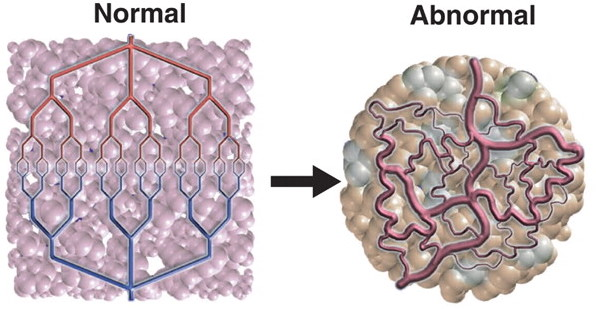
\includegraphics[width=0.65\textwidth]{images/BloodVessels.jpg}
\caption{\textit{Left, healthy vasculature. Right, tumour abnormal vasculature\cite{Jain58}} \label{BloodVessels}}
\end{figure}


\noindent To achieve this ambitious goal, a comprehensive understanding of the haemodynamics in micro- circulation is required for both the beginning and progression of the disease. However, it is very difficult to attain such knowledge solely through experiments due to the immense complexity of micro-circulatory blood flow in the human body. Furthermore, it still remains unclear how the different structural features of the micro-vessels and the components of blood (E.g. white blood cells, platelets etc; see Figure \ref{BloodComponents}) affect blood flow, tissue dysfunction and tumour growth. This also applies to finding out how these contributing factors can be exploited in disease therapy and other bio-engineering applications. Such complexity gives rise to major obstacles and challenges despite the recent technical advances in experimental techniques along with the breakthroughs made in developing animal models.\cite{PriesAR1994RtBF, Pries2000TheLayer, PRIES198981, Pries1992BloodHematocrit} \\

\noindent Recent computational techniques\cite{Noguchi14159, DoddiSaiK2009Tcmo, Freund2014, Balogh2018, 2020Charles} for blood flow modelling have developed rapidly and act as a powerful tool to analyse the micro-circulatory haemodynamics within complex geometries (E.g. flow distribution, RBC partitioning, haematocrit heterogeneity, wall shear stress difference). Such techniques have also become more reliable to validate some of the well-known blood flow phenomena (e.g. Zweifach-Fung effect, F{\aa}hr{\ae}us-Lindqvist effect and plasma skimming) observed in previous experimental studies. Furthermore, the recent technical advances in intravital microscopy and measurement techniques have accelerated the progress in characterising the blood flow behaviours in micro-circulations. However, it is still beyond our reach to attain a fully established model of the micro-circulatory blood flow including all biophysical or biochemical elements due to the constraints of computational power. \\

\noindent For this reason, several reduced-order models (ROM) were introduced to simplify the mathematical calculations and provide reliable predictions of haemodynamic quantities with satisfactory accuracy and lower computational expense. Various simplifications have also been made to existing models and some of the most common simplifications implemented were either dimensionality reduction or rheology homogenisation.\cite{CharlesPhDThesis2020} Dimensionality reduction relates to applying two-dimensional (2D) models to describe three-dimensional (3D) effects observed in \textit{in vivo} and \textit{in vitro}. Rheology homogenisation approximates blood flow as a homogeneous non-Newtonian fluid to simplify the intrinsic heterogeneity of blood arising from the non-continuum effects.\cite{CharlesPhDThesis2020} Another common simplification made is assuming negligible inertial effects due to low Reynolds number under Stokes flow regime in micro-circulations. 


\begin{figure}[H]
\centering
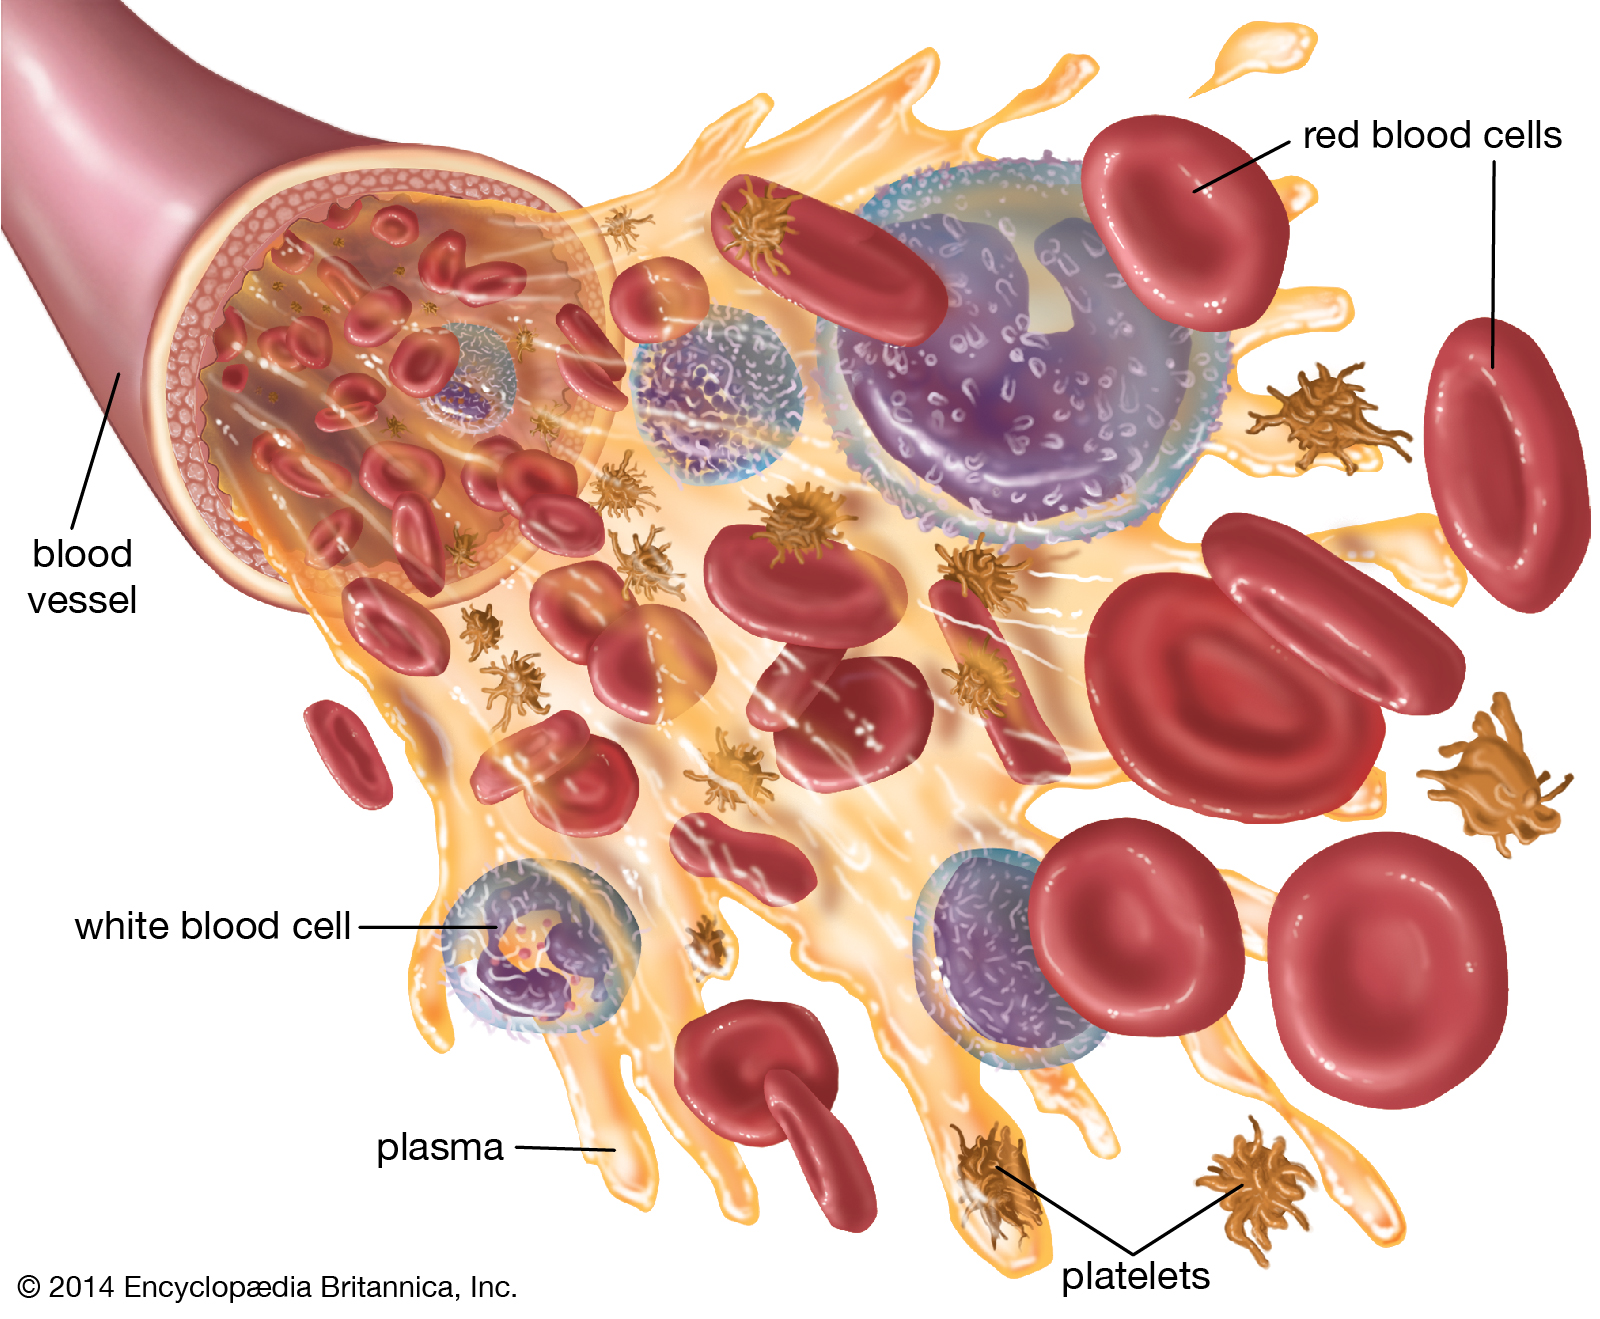
\includegraphics[width=0.65\textwidth]{images/BloodComponents.jpeg}
\caption{\textit{Blood is made up of multiple components, including red blood cells, white blood cells, platelets, and plasma. \cite{whitebloodcells}} \label{BloodComponents}}
\end{figure}


\noindent Despite decades of extensive research and theoretical studies in this field, multiple effects still remained unexplained from the predictions obtained in these simplified models (E.g. 2D models or continuum flow models). The conventional assumptions (E.g Poiseuille law, symmetrical haematocrit profile or time-average accuracy) also do not take into account certain key cellular characteristics of blood at micro-scale which affects the quantification of certain measuring flow variables like apparent viscosity and wall shear stress. Therefore, there are still significant challenges in quantitatively describing the micro-circulatory blood flow and pinpointing the potential haemodynamic mechanisms in micro-scale systems. \\


\noindent This brings us to the purpose of the current research project which is to analyse and identify the correlations from existing particle-based simulation data of blood flow in 3D complex microvascular networks.\cite{2020Charles} It was also investigated how well the predictions from some of the established ROMs developed by Pries et al.\cite{A.R.Pries2005Mbvi, PriesAR1994RtBF} are matched against simulation data in order to identify the existence of certain haemodynamic effects in the studied networks. Furthermore, distinct correlations were identified to take note of the contributing factors for the observed effects found from simulation data. This results to suggesting what are the next steps required to develop a reduced-order model that captures the observed effects on a network level in micro-circulations. Therefore, the overall work in this research project helps to provide a better understanding of the blood flow behaviours in micro-vessels based on fluid mechanical perspectives. 










%----------------------------------------------------------------------------------------
%	LITERATURE REVIEW SECTION
%----------------------------------------------------------------------------------------
\newpage
\section{Background of Blood Flow Distributions in the Microcirculation}

\noindent This section presents an introduction of micro-circulatory blood flow and a literature review of the blood flow distributions in micro-circulations. The blood flow in micro-circulations has several distinctive features\cite{BloodFlowSecomb, AnnualReview} that are discussed in this section to provide a basic understanding of the different physical mechanisms and contributing factors observed from past studies. Several haemodynamic effects observed in microvascular networks are covered in Section \ref{HaemodynamicEffects} along with an overview of the current challenges in reduced-order models for computational studies. Last but not least, the research gaps in the literature are identified and this includes a brief discussion on the physical perspectives of RBCs and blood flow in microvascular networks. 

\bigskip

\subsection{Mechanical Properties of Red Blood Cells}
\label{MechanicalPropertiesOfRBC}
\noindent Red blood cells (RBCs) in the blood are specialised cells responsible for transporting O$_{2}$ to respiring organs and carrying CO$_{2}$ to the lungs, where it gets excreted.\cite{redbloodcells} Without any presence of external stress, the shape of a normal human RBC is widely known to be a biconcave disk with a diameter and thickness of roughly 8 $\mu$m and 2 $\mu$m respectively.\cite{Jung1971PermeabilitySugars} However, there are also abnormally-shaped RBCs because of certain medical conditions or genetic mutations which alter the normal RBC morphology. (see Figure \ref{RedBloodCell} for illustration.)

\begin{figure}[H]
\centering
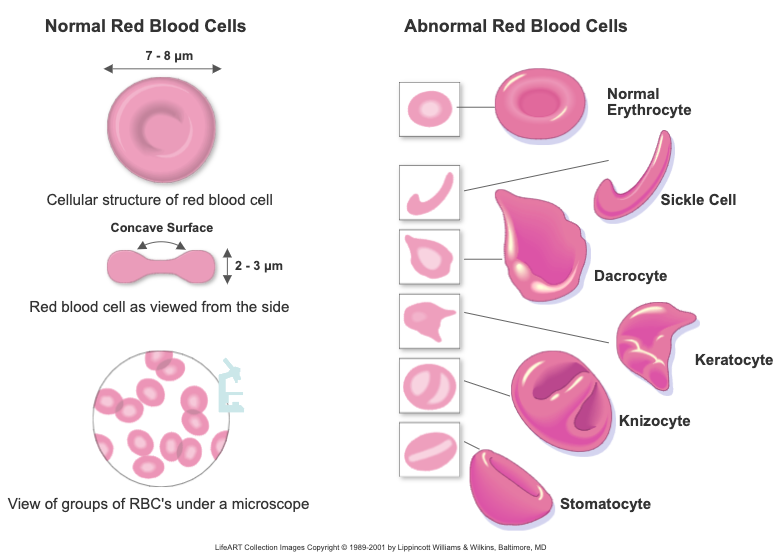
\includegraphics[width=0.9\textwidth]{images/RedBloodCellDescription.png}
\caption{\textit{An illustration of the shapes and sizes for a normal red blood cell along with the different types of abnormal red blood cells.  \cite{RedBloodCellsDescription, LifeART2000}} \label{RedBloodCell}}
\end{figure}

\noindent The RBC membrane from a mechanical perspective is perceived as a thin and highly deformable viscoelastic shell that contains a concentrated solution of haemoglobin. It behaves like an incompressible fluid with an approximate viscosity of 7 mPa s.\cite{chien1975red} The RBC membrane is critical to the deformability of RBCs as the viscoelastic properties of the protein cytoskeleton primarily influence the mechanical reaction of the RBC membrane to shear deformation.\cite{EvansE.A1976Mv} Unlike the RBC, the viscosity of the suspending medium (i.e. plasma) is usually around 1.2 mPa s and it behaves like a Newtonian fluid in micro-circulations. Given that the two primary components of blood are RBCs and plasma, the presence of RBCs is a major contributing factor to blood viscosity and hence, affecting the blood flow behaviours through extremely narrow capillaries. \\ 

\noindent In essence, the above description of the mechanical properties of RBCs summarises the essential keynotes for simulating the behaviour of RBC suspensions in micro-vascular networks under a specific given set of flow conditions. As a result, the RBCs in the simulation was modelled as a deformable capsule with a thickness of zero hyper-elastic membrane containing a viscous fluid called cytoplasm which consists of haemoglobin. In practice, these simulations are challenging due to the mechanical complexity of fluid-solid interactions especially when dealing with a large number of particles interacting among one another in a fluid.

\subsection{Difference between \textit{in vivo} and \textit{in vitro} experiments}
\label{DifferenceIn_Invivo_Invitro}
\noindent Numerous \textit{in vivo} and \textit{in vitro} studies\cite{LIPOWSKY1980297, PRIES198981, CARR1990179, PriesAR1990BFiM, PriesAR1994RtBF, SmithMichaelL2003Nmra, Sherwood2014, Roman2016, Mantegazza2020} have been conducted over many decades to examine blood flow behaviours and investigate the partitioning of RBCs at vascular bifurcations. Many of these studies have demonstrated that across the networks, the RBCs are often not distributed with the same proportion as the blood flow. However, both methods of scientific studies are very different because \textit{in vivo} studies refers to performing experiments within a living organism (i.e. real blood vessel segments) whereas, for \textit{in vitro} studies, it refers to conducting experiments in a controlled environment such as glass capillary tubes. This affects the interpretation of both results given that the \textit{in vitro} experiments cannot replicate the conditions that occur inside a living organism. Therefore, it is frequently observed that the velocity profiles, haematocrit distributions and blood viscosity do vary substantially between \textit{in vivo} and \textit{in vitro} experiments. \\

\noindent For \textit{in vitro} studies, most of these experiments using long straight glass tubes generally produce symmetrical RBC distributions, unlike \textit{in vivo} studies where asymmetric RBC distributions are more frequently observed.\cite{Sherwood2014} In addition to this, blood viscosity was often found to be several factors lower in \textit{vitro} compared to \textit{in vivo} environments.\cite{Pries2000TheLayer, A.R.Pries2005Mbvi} This is due to the presence of endothelial surface layer (ESL) found within the interior blood vessel walls, unlike \textit{in vitro} experiments where the glass capillary tubes have smooth interior surfaces. The ESL consists of squamous endothelial cells, which reduces the effective width of the lumen and largely hinders the flow of plasma and RBCs.\cite{Pries2000TheLayer, WeinbaumSheldon2007Tsaf} Therefore, the results obtained from both \textit{in vivo} and \textit{in vitro} experiments have indicated that the significant difference in the measured flow resistance values is caused by ESL. This makes it very challenging to accurately model the blood flow behaviours and RBC distributions in micro-circulations. \\

\noindent To summarise, \textit{in vivo} experiments are done within living organism under physiological conditions which makes it time-consuming and expensive to perform. In comparison, \textit{in vitro} experiments refers to the technique of performing a given procedure in controlled laboratory conditions that requires lesser time and is cheaper to perform but are limited to their functions as they will need further validation from \textit{in vivo} results. 

\subsection{Blood Vessel Topology and Geometries}
\label{Topology_Geometries}
\noindent Previous cellular-scale modelling studies consider blood flow in simple geometries like long and uniform circular cross-sectional branches or in some instances complex geometries like vascular networks. The geometrically complex branching network of micro-vessels in large-scale micro-circulations pose a great challenge for researchers to model and reconstruct these vascular networks. The complex architecture of vascular networks is often characterised by bifurcating, merging and winding vessels.\cite{fung2013biomechanics} On top of this, different organs have different types of network topology. For example, blood vessels in the retina and kidney have a tree-like topology\cite{LiYiwen2008Dlav} while vessels in muscles form arcade-type planar networks\cite{KianiM1994Fimb, tawfik2013mathematical}(see Figure \ref{BloodNetworkTopology} for illustrations). For tumours, the blood vessels can have trifurcations and short-length shunts which further increases the complexity of the network.\cite{TumorMicrovasculature} Therefore, these geometrical differences can cause significant deviations in the haemodynamics of long straight branches compared to a vascular network.

\begin{figure}[H]
\centering
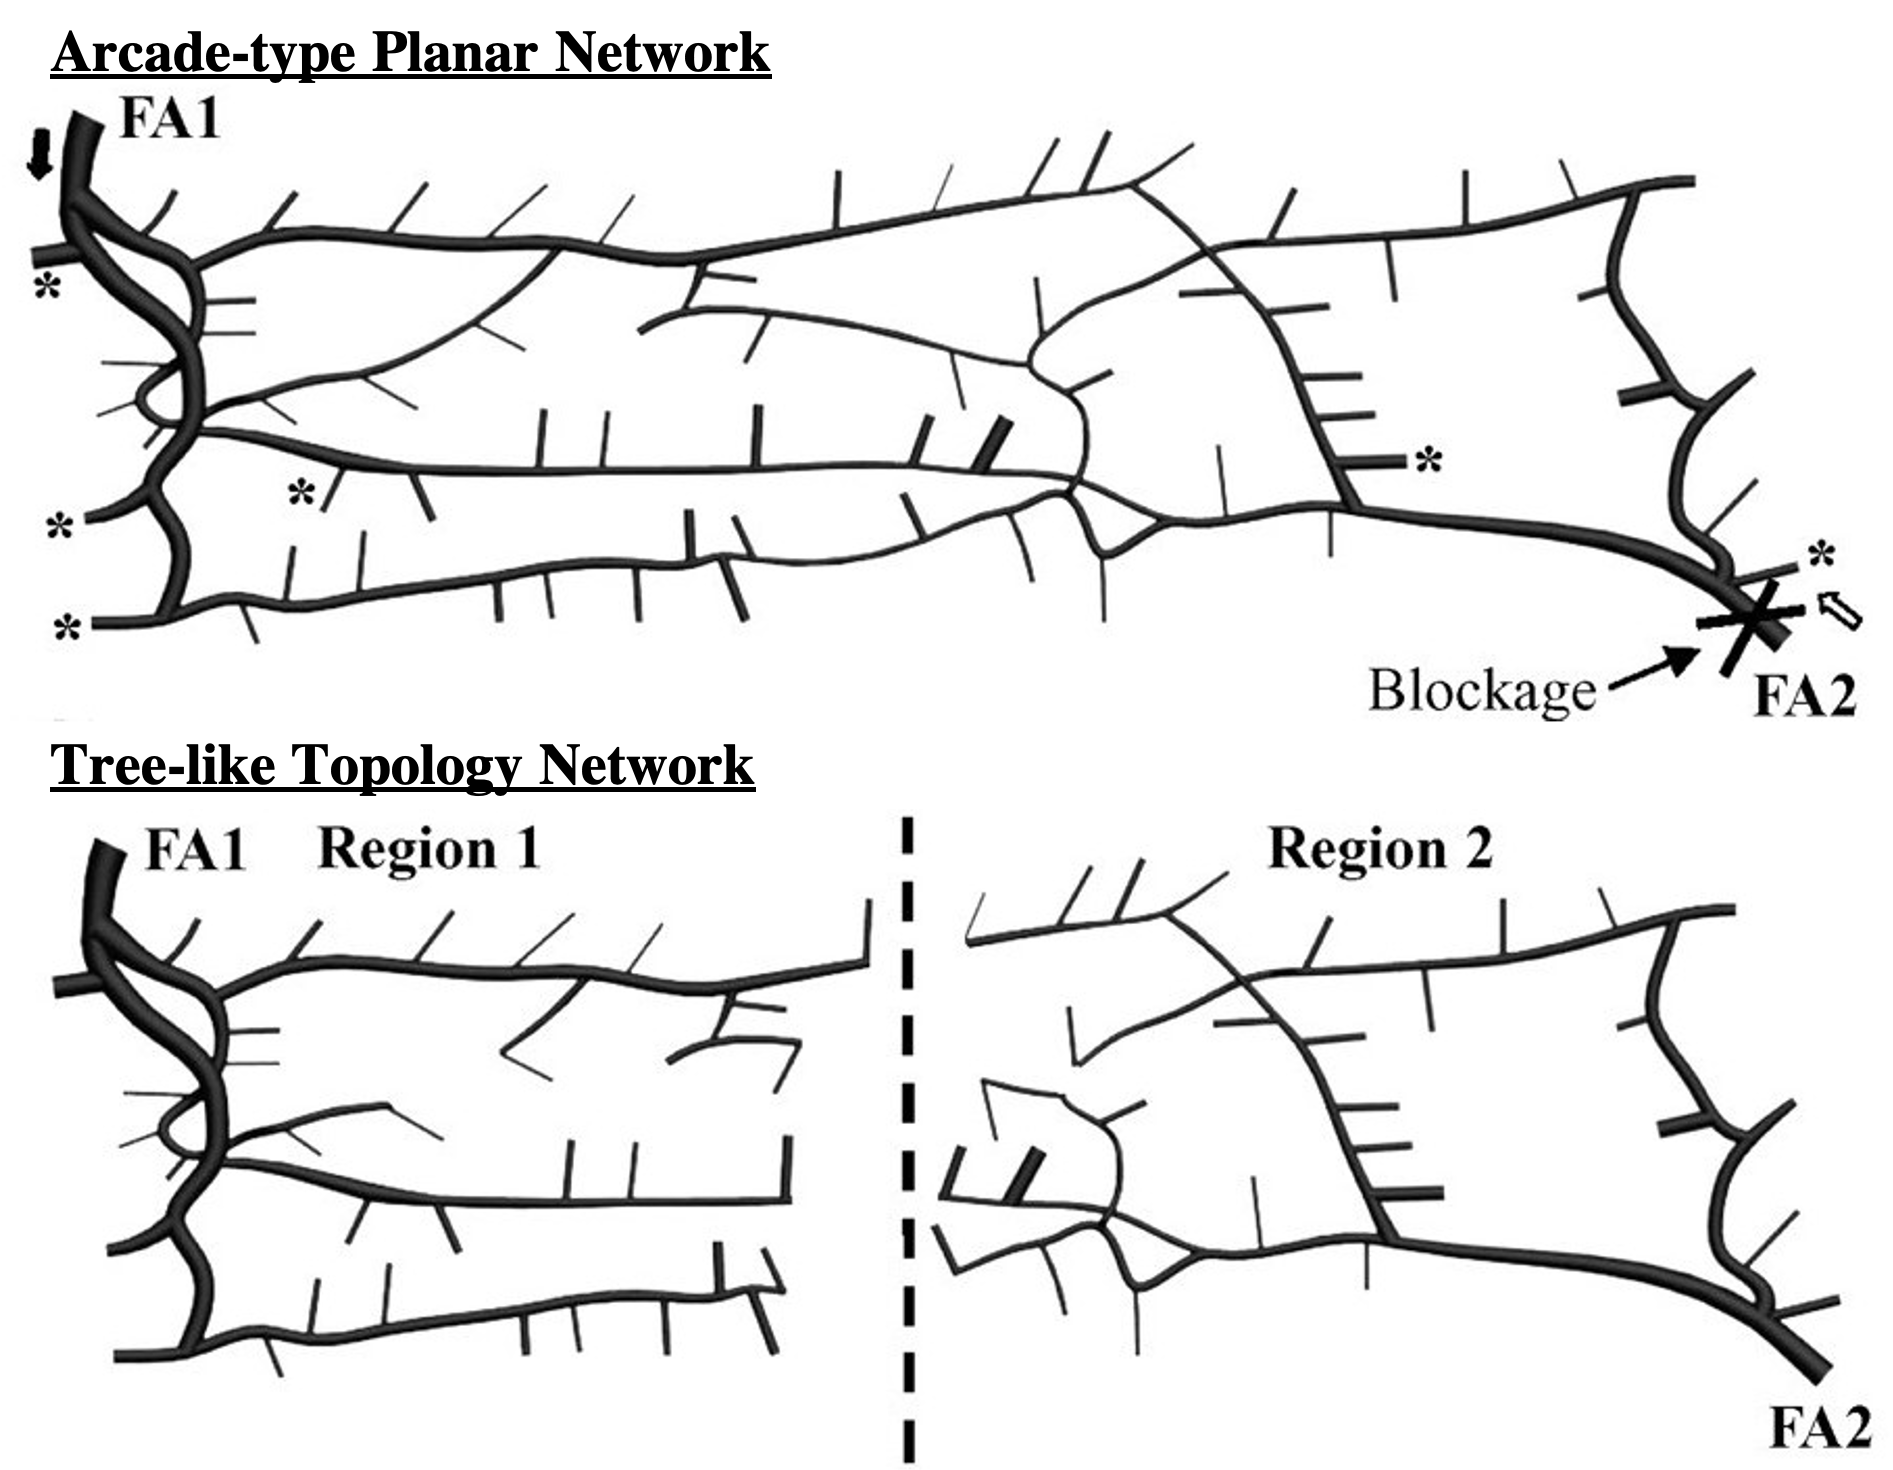
\includegraphics[width=0.6\textwidth]{images/TopologyNetworks.png}
\caption{\textit{Computer visualisation of an arcade-type and two-tree blood flow networks.\cite{NetworkTopology2005} FA1 and FA2 represent the branches of feed arteries with arrows indicating the direction of flow. Arcade outflows are shown with an asterisk (*) and all other open-end vessels are transverse arterioles.} \label{BloodNetworkTopology}}
\end{figure}

\subsubsection{2D \& 3D Simple Networks}
\noindent In general, most of the cellular-scale modelling studies conducted were investigating in either two- dimensional (2D) or three-dimensional (3D) computational simulations where the geometry of the networks were either idealised or obtained from the reconstruction of \textit{in vivo} images.\cite{PriesAR1990BFiM, reichold2011cerebral, Gould2015HematocritNetworks, Balogh2018, CharlesPhDThesis2020} However, there are considerable differences between both dimensional approaches. For example, there is a significant size difference between 3D to 2D translations because the RBC takes up more cross-sectional space in a 2D environment compared to 3D. Furthermore, using 2D models to replicate data from 3D realistic systems would neglect the trade-off effects and slow down RBC migration.\cite{Barber2011SimulatedPartitioning} Hence, this affects the RBC trajectories and might exaggerate the size of obstruction effects in 2D modellings.\cite{Xiong2012Two-dimensionalEffects} Another issue would be not accounting for the in-plane shear elasticity of RBC membrane given that experiments have emphasised the importance of membrane shear elasticity in modulating blood rheology based on its effect on RBC morphology and dynamics.\cite{PhysRevLett2018} \\

\noindent Whereas for simplified 3D networks, the 3D models are able to address more crucial factors such as RBC deformability and fluid flow dynamics with adequate accuracy. In addition to this, 3D models are capable of capturing both the complex physiological architecture and the micro-physics at a cellular scale. This will not only elucidate haemodynamic mechanisms at the micro-scale but also discover new insights from novel phenomena that can't be detected from 2D models.\cite{Balogh2017DirectNetworks} However, conducting these theoretical studies of RBC transport in 3D networks are very costly as it requires a substantial amount of computational time and expenses to fabricate and generate these 3D models, unlike the 2D models.\cite{KRUGER20113485, Zavodszky2017, BaloghPeter2019} \\


\noindent As a whole, when implementing the 2D models to represent a 3D system, there will be a few inevitable limitations given that not all factors influencing the RBC partitioning and blood flow behaviours are considered. This is due to the approximations of a 2D system that does not truly represent a 3D micro-vascular network. Therefore, this highlights the importance of understanding both the vessel geometries and microphysics at a cellular scale in order to evaluate the haematocrit distribution across the network. On the other hand, these 2D models can still provide a good template for us to start understanding some of the cellular interactions and blood flow behaviours occurring in vascular networks.


\subsubsection{3D Complex Architectural Networks}
\noindent For complex 3D realistic/idealised micro-vascular networks, the investigation of RBC suspensions in such networks serves as an advanced study of micro-circulatory haemodynamics within complex geometries. It allows us to elucidate the microscopic behaviour of RBCs at bifurcations and capture phase separation phenomenon such as plasma skimming effects.\cite{Krogh1921, PRIES198981} Furthermore, the findings from these simulations may offer new insights to propose potential haemorheology mechanisms that describe the subtle behaviour of RBCs circulating in blood flow at the micro-scale. However, it is also not a trivial task to examine the physical effects that dictate the RBC dynamics within non-circular micro-vessels, given that there are a plethora of effects occurring simultaneously in a network of micro-vessels. This suggests adopting an image-based simulation framework\cite{2020Charles} to model the blood flow in microvascular networks and formulate simplified yet robust reduced-order models via data accumulation of these micro-circulatory simulations. This will not only increase the proficiency of simulating physiological micro-vasculatures but also potentially detect or predict haemodynamic disorders within human tissues or organs in the future. 

\subsection{Mechanisms that affect Radial Distribution of RBCs}
\label{BloodFlowMechanisms}
\noindent Previous experimental and numerical studies in micro-circulation have demonstrated that certain physiological phenomena are associated with the motion of RBCs across diverging bifurcations (see Figure \ref{FluidMechanicalPhenomena}). In these diverging bifurcations, the RBC partitioning does not necessarily distribute proportionally to the partition of blood flow which leads to a high degree of heterogeneity within the network of micro-vessels. These phenomena contribute to the formation of a cell-free layer (CFL) near the interior vessel walls which not only cause lateral migration of RBCs away from vessel walls but also defines the distinctive blood flow properties in micro-vessels.\cite{AnnualReview} 

\begin{figure}[H]
\centering
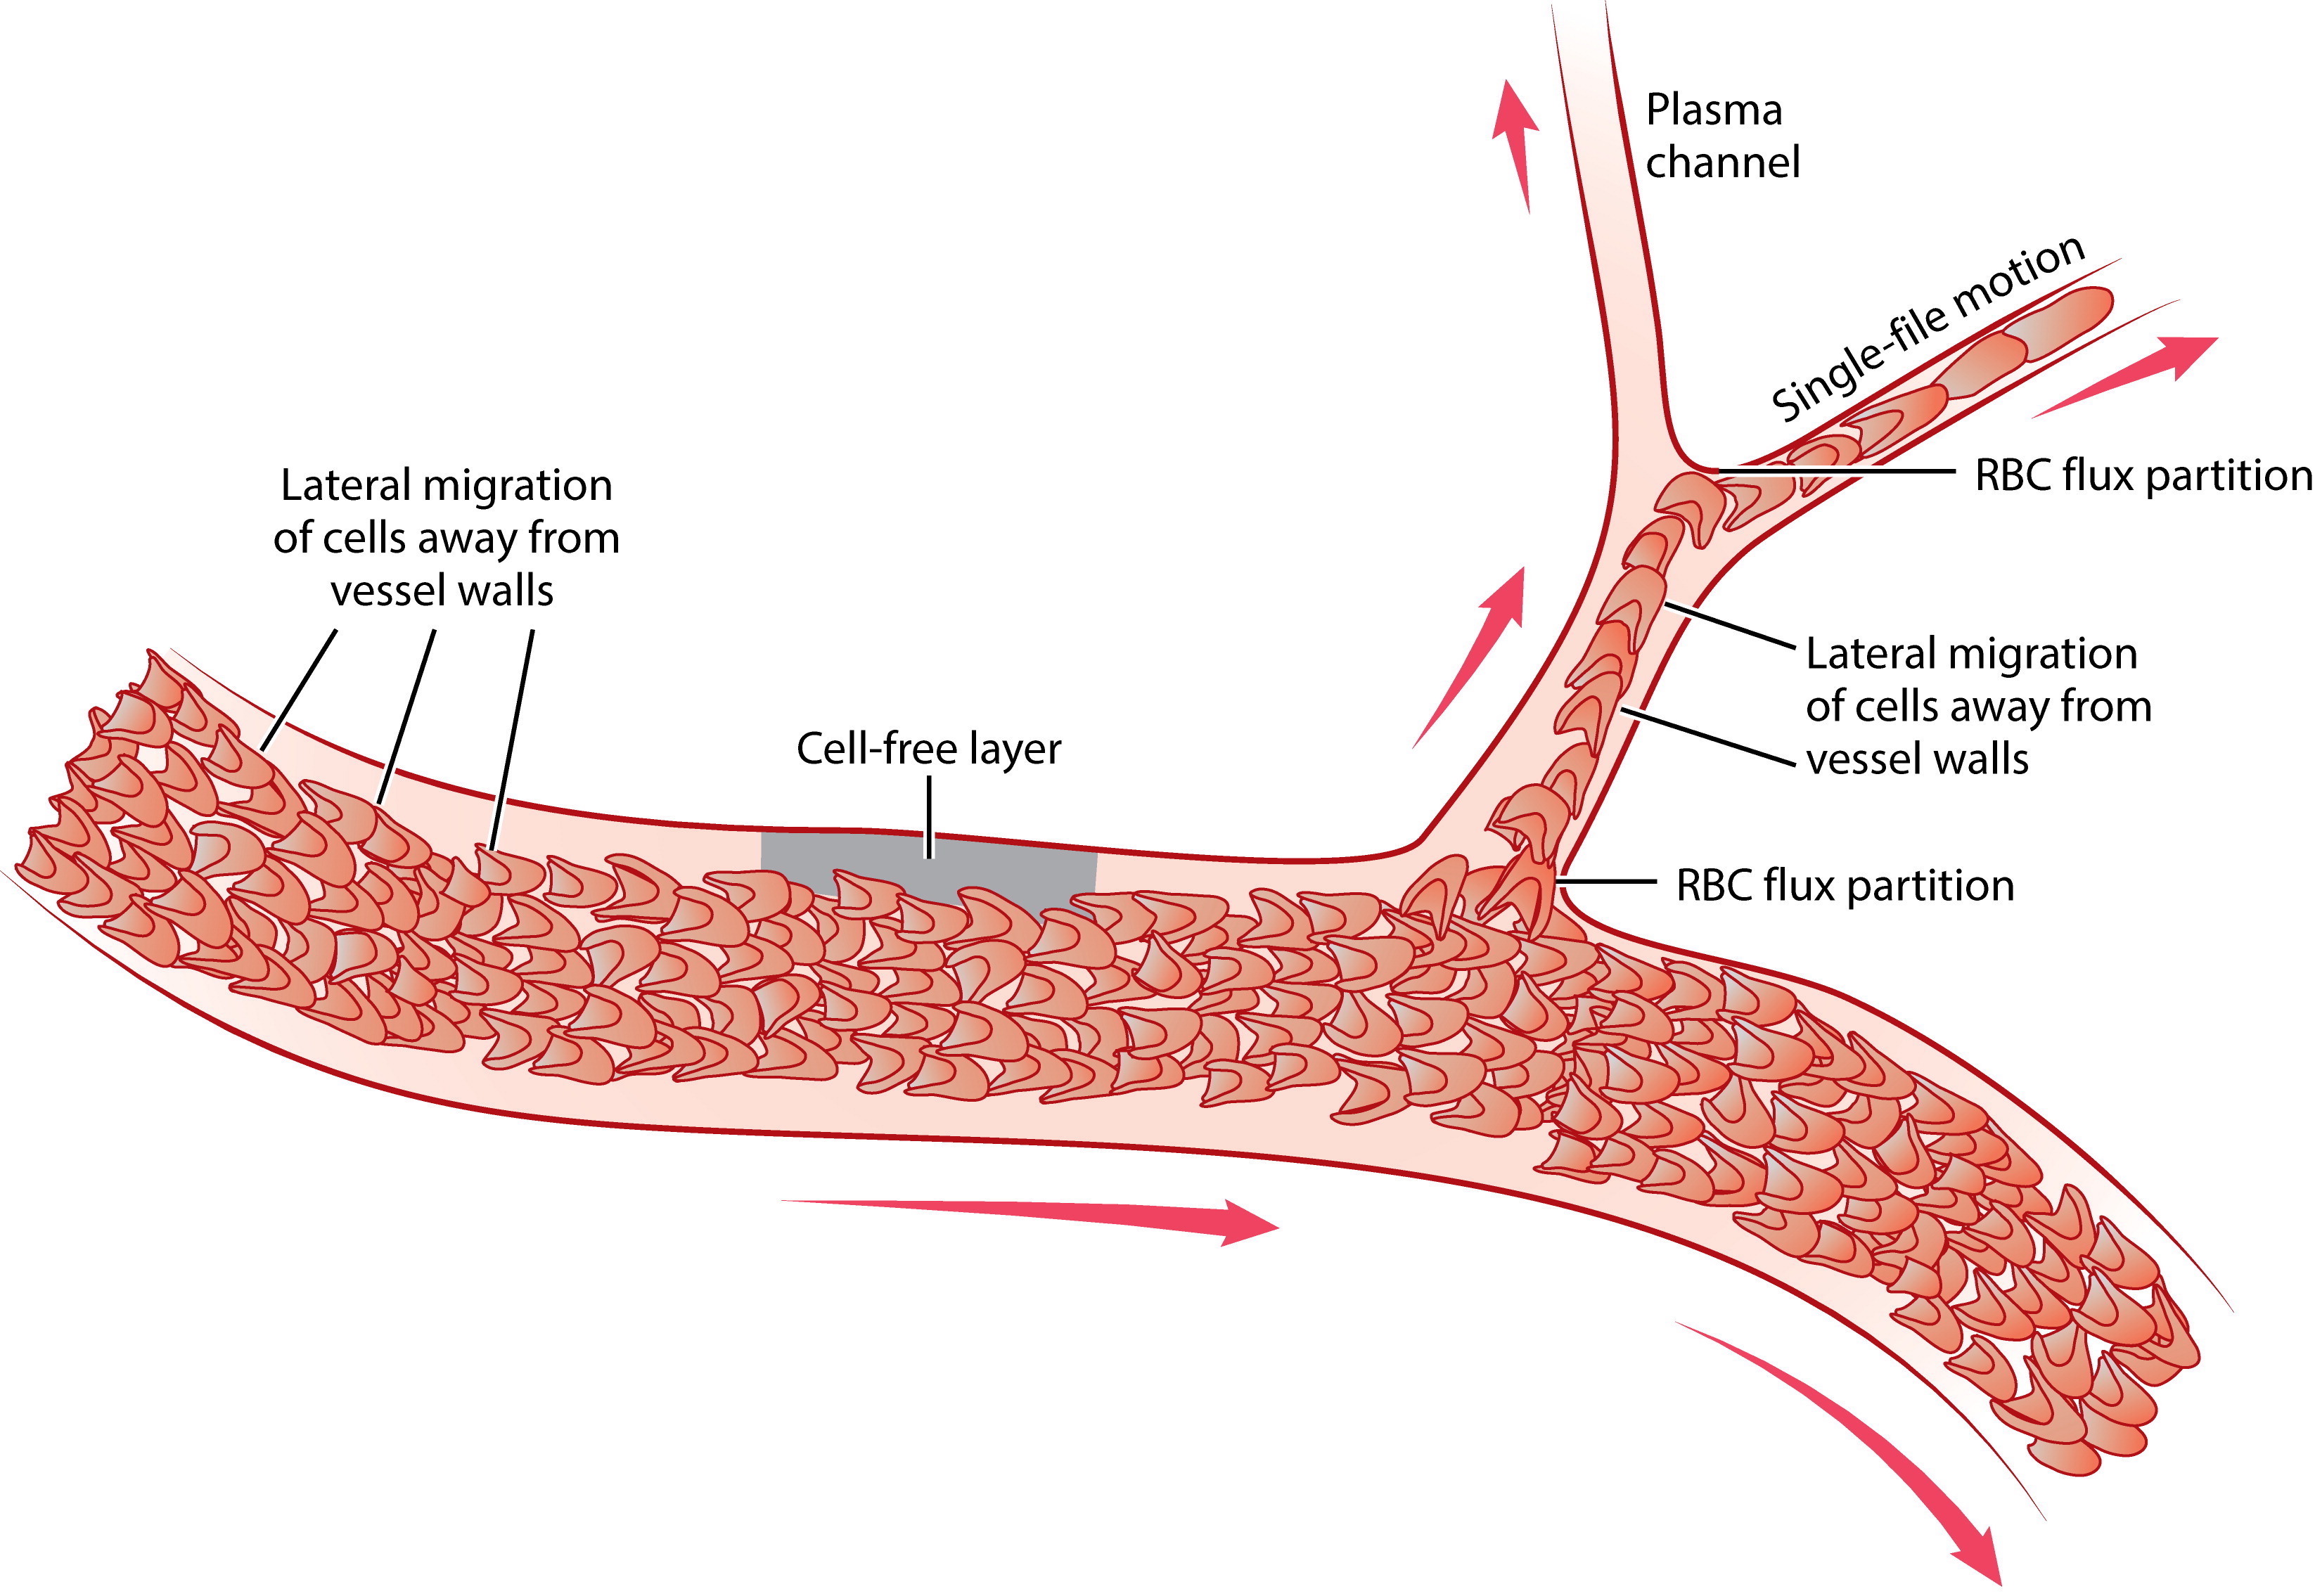
\includegraphics[width=0.85\textwidth]{images/PlasmaSkimming.jpeg}
\caption{\textit{Different fluid mechanical phenomena caused by uneven distribution of red blood cells at diverging bifurcations.\cite{AnnualReview}} \label{FluidMechanicalPhenomena}}
\end{figure}


\noindent One example is the tendency for RBCs flowing near the vessel walls to migrate away from the walls due to their deformability, hence forming a cell-free layer near the walls and altering the RBC distribution downstream.\cite{PhysRevLett} Another plausible physical mechanism is due to the Poiseuille velocity profile's curvature in tube flow which causes the tendency of RBC migration towards the centre line of the flow (assuming wall effects are neglected).\cite{2020Charles} However, the effect from the velocity profile curvature only dominates significantly under dilute suspensions and not concentrated suspension conditions. This is because both the shear-induced dispersion effect and cell-to-wall interactions are more prevalent mechanisms that govern the radial distribution of RBCs in microvascular networks.\cite{CoupierG2008Nlmo} The following subsections highlight the different plausible mechanisms that contribute to the radial distribution of RBCs in multi-file flows.


\subsubsection{Cell-to-Cell Interactions}
\noindent An investigation of the effects of cell-to-cell mechanical interactions is important to understand the RBC partitioning behaviours in diverging bifurcations. In reference to a 2D computational modelling study conducted by Barber et al.\cite{Barber2011SimulatedPartitioning}, three main types of two-cell interactions were found that can affect the RBC partitioning. The first interaction is a "trade-off" mechanism where the front cell enters a child branch, and the following cell enters the opposite child branch. For the second interaction, it is a "following" mechanism that occurs when the rear cell enters the same branch as the front cell. Lastly, "herding" is the third mechanism observed where the front cell enters the same branch as the rear cell.  \\

\noindent The "trade-off" mechanism appears to occur most frequently unlike the other two mechanisms due to continuity of flow and conservation of mass law. This causes a tendency towards having a more uniform haematocrit partitioning in the downstream branches as haematocrit increases although the opposing effects of "following" and "herding" mechanisms do slightly counteract this tendency.\cite{Barber2011SimulatedPartitioning} However, do take note that these mechanisms mentioned above are only considering the effects of two-cell interactions in 2D systems and under dilute suspension conditions. Whereas under physiological conditions with 40\% hematocrit, the collisions between RBCs will occur more frequently due to the strong hydrodynamic interactions that oppose the migration to the centreline and cause the RBCs distribution to broaden in parent branches.\cite{PRIES198981} Therefore, there is a greater tendency for concentrated RBC suspensions under shear flow conditions to migrate across the flow and towards the walls in the of decreasing concentration. This phenomenon is referred to as the shear-induced dispersion effect.\cite{Leighton1987MeasurementSpheres, Pranay2012, HariprasadSecomb2014} 



% This will fluctuate the lateral velocities and drive a diffusion-like motion of the particles, with a net flux down the concentration gradient. Therefore, the development of quantitative models are required to observe other types of interactions involving multiple cells at higher haematocrit and in 3D systems. 


\subsubsection{Cell-to-Wall Interactions}
\noindent On the other hand, previous studies of the motion of RBCs under shear flow near a solid boundary have also demonstrated that under the Stokes flow regime, the RBC suspensions in tubes tend to migrate away from the interior walls in 3D simulations.\cite{CoupierG2008Nlmo, DoddiSaiK2009Tcmo} This is primarily due to the effects of RBC deformability to cell trajectories that causes this migration phenomenon to occur\cite{PhysRevLett}. However, the complete mechanistic understanding of this phenomenon is difficult as multiple effects are involved. This is because there is no concrete evidence to prove that the deformable RBCs close to the walls will consistently migrate away from the wall in all scenarios. \\

\noindent However, there are certain distinct observations found in several experiments that do partially answer the physical mechanisms related to this migration phenomenon. For dilute suspensions under shear-flow conditions, tank-treading motions were observed in numerous experiments where these close-wall tank- treading RBCs tend to migrate away from the interior walls due to hydrodynamic lift force which leads to axial drifting.\cite{Olla_1997A, Olla_1997B, PhysRevLett.83.876, PhysRevLett2002, PhysRevLett} Therefore, this gives rise to the development of CFL where it serves as a lubricant film that decreases the apparent viscosity of blood in the tube and also has prominent implications for blood flow in micro-circulation.\cite{feng_weinbaum_2000, CharlesPhDThesis2020}


% If the suspending medium has a viscosity similar to that of plasma, RBCs exhibit tumbling motions with the vorticity vector of the shear flow as the axis (Keller & Skalak 1982, Barthes-Biesel 2016). Migration away from the wall is still observed in this case (Grandchamp et al. 2013).

% https://journals.aps.org/prl/abstract/10.1103/PhysRevLett.98.188302
% a swinging motion of the RBC was discovered in several experiments and this motion was characterised by an oscillating inclination angle on top of the classic tank-treading motion


\subsubsection{Initial RBC Distribution in Parent Branch}
\label{InitialRBCDistributionInPB}
\noindent Previous experimental studies have established several well-known models\cite{PRIES198981, GuibertR2010ANAt, Gould2015HematocritNetworks, LeeTae-Rin2017Gpsm} that describe the plasma skimming effects under a central assumption of axisymmetric haematocrit profile in the parent branch of each bifurcation. However, substantial haematocrit asymmetry has always been observed in the parent branches across numerous studies.\cite{Zhou2021EmergentBifurcations, 2020Charles} This suggests that without specific knowledge of the cross-sectional RBC distribution in a given branch, it will be challenging to have an accurate prediction of the downstream blood flow behaviours across the networks. Furthermore, a recent study in tumour vascular networks has pointed out other sources of haematocrit asymmetry such as the reduced interbifurcation distance and complex vessel topology which drives oxygen heterogeneity in solid tumours.\cite{Bernabeu2020AbnormalOxygenation} Apart from haematocrit asymmetry, the uneven velocity profile in capillary vessels can also occur as the parabolic velocity profile can become skewed over time due to the presence of RBCs.\cite{2020Charles, JosephAby2019Isbf, Balogh2018, Balogh2017DirectNetworks} Therefore, both asymmetries in velocity and haematocrit profiles in the parent branch can significantly affect the radial distribution of RBCs in the downstream branches and across the microvascular networks.


\subsubsection{Cellular Mechanisms: Lingering \& Jamming}
\noindent The rapid improvement in computational studies has enabled researchers to identify and analyse cellular-scale mechanisms underlying the time-dependent partitioning behaviours. Recent studies of RBC partitioning through simplified and complex geometries\cite{wang_sui_salsac_barthes-biesel_wang_2016, Balogh2018, Balogh2017DirectNetworks} have observed cell lingering and jamming effects occurring across the microvascular networks. The RBCs lingering dynamics at vascular bifurcations results in temporary and partial obstructions to the blood flow in both child and parent branches as this also lead to cell jamming at the bifurcations. As a consequence of these mechanisms, this leads to reverse partitioning behaviours occurring across the microvascular networks.\cite{Balogh2017DirectNetworks} Furthermore, the mechanisms are also associated with the asymmetric distribution of RBCs in the downstream bifurcations due to the pilling up of RBCs at the upstream bifurcations which results in a haematocrit reduction in the child branches.\cite{Balogh2018} (see Figure \ref {CellularMechanisms} for illustration purposes.)

\begin{figure}[H]
\centering
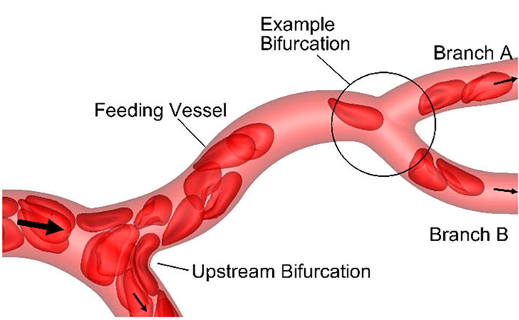
\includegraphics[width=0.85\textwidth]{images/CellularMechanisms.png}
\caption{\textit{An illustration of a reverse partitioning behaviour due to cellular mechanisms in a successive bifurcation from micro-vascular networks. The pilling-up of RBCs in the upstream bifurcation affects the RBCs entering the feeding vessel to shift towards the left-hand side of the vessel which results to increasing the fractional RBC flux in branch A.\cite{Balogh2018}} \label{CellularMechanisms}}
\end{figure}

\noindent However, these results from recent studies\cite{Balogh2018, Balogh2017DirectNetworks, KihmAlexander2021LDiM} have not yet been compared to a detailed analysis of the lingering effects in \textit{in vivo} experiments. All of the lingering effects observed were described based on \textit{in silico} experiments which lack the proper quantification and full understanding of this lingering effect in \textit{in vivo} experiments. Therefore, further investigations will be required in the future to elucidate the fundamental dynamics of the cell lingering effects under \textit{in vivo} conditions. This is because the impact of cell lingering on the blood flow behaviour can lead to severe implications on the entire micro-vascular network as it can significantly disrupt the radial distribution of RBCs across multiple micro-vessels.  



% We have provided evidence to show that these lingering events cause a breakup of trains of RBCs as well as redistribution in the branching vessels. Even though these effects seem to be rather fine grained, the impact on the whole organism may be severe, given the importance of blood flow to the health state.x


\subsubsection{Effects of the Endothelial Surface Layer}
\noindent According to numerous \textit{in vivo} investigations\cite{Pries2000TheLayer, ReitsmaSietze2007Tegc, WeinbaumSheldon2007Tsaf, SmithMichaelL2003Nmra, A.R.Pries2005Mbvi}, there was strong evidence of endothelial surface layer (ESL) existing near the interior surfaces of the blood vessels (see Figure \ref{EndothelialSurfaceLaye}). It was suggested that the interactions between the plasma and membrane-bound glycocalyx were responsible for the formation of ESL.\cite{Pries2000TheLayer} The ESL consists of squamous endothelial cells, which reduces the effective width of the lumen and largely hinders the flow of plasma and RBCs.\cite{Pries2000TheLayer, WeinbaumSheldon2007Tsaf} This shows that the presence of the ESL will have a significant effect on the haemodynamic components in micro-circulation such as flow resistance where the effect amplifies in micro-vessels especially for extremely narrow diameters which substantially increases the flow resistance. Additionally, results from Pries et al.\cite{PriesAR1990BFiM, PriesAR1994RtBF, Pries2000TheLayer} experiments have proven that the presence of ESL greatly affects the haematocrit distribution in complex blood flow networks. Therefore, this highlights the importance of considering ESL in \textit{in silico} experimental modellings as it will aid researchers to gain a further understanding of the mechanical interactions between the RBCs and ESL in complex microvascular networks. 

\begin{figure}[H]
\centering
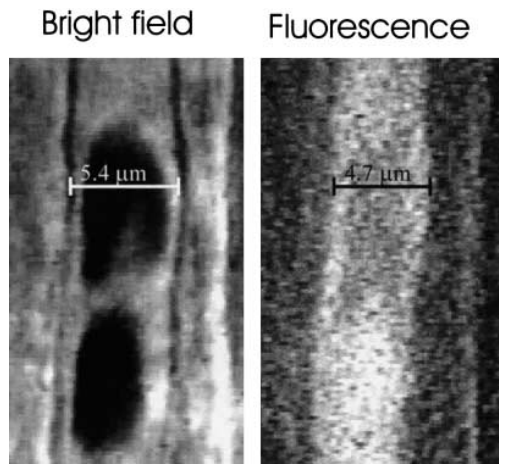
\includegraphics[width=0.7\textwidth]{images/EndothelialSurfaceLayer.png}
\caption{\textit{Existence of the endothelial surface layer via observations from a capillary in the hamster cremaster recorded during intravital microscopy. Under a bright field illumination shows the anatomical width of the capillary (Right) while under a fluorescence illumination identifies the width of the plasma column (Left). The difference suggests the presence of the endothelial surface layer.\cite{Pries2000TheLayer}} \label{EndothelialSurfaceLaye}}
\end{figure}


\subsubsection{Presence of Other Suspended Particles}
\noindent Although RBCs and plasma are the two main dominant components in blood, there are several other biologically important types of cells that should be considered such as white blood cells (WBC) or platelets.(see Figure \ref{BloodComponents}) To perform their biological functions, the ability for these particles to reach the micro-vessel walls is crucial as the WBCs are responsible for the body's responses to injuries and infections while the main function for platelets is to stop bleeding from damaged blood vessels. Therefore, the fluid dynamic interactions with RBCs affects these particles lateral motion within micro-vessels as numerous experiments\cite{GoldsmithHarryL1984Moli, NobisU1985Rdow, TangelderG1985} and computational studies\cite{FedosovDmitryA2014Wbcm, FreundJonathanB2007Lmia, VahidkhahKoohyar2014PDiT, MehrabadiMarmar2015ACMf, PhysRevLett.108.028104} have observed that both of WBCs and platelets are preferably distributed near the walls of the vessels. This migration of RBCs away from vessel walls primarily depends on the RBC's deformability which also induces the outward migration of more rigid particles like WBCs and platelets.\cite{PhysRevLett.109.108102} Therefore, this highlights the dependence of other suspended particle migrations on the hydrodynamic interactions of RBCs within the vessel walls as this affects the radial distribution of RBCs across the microvascular networks.

 

% Different Types of Radial Distribution of RBCs in Micro-circulation Network: 
% -> Size Exclusion Effect
% -> Wall-Induced Lift
% -> Shear-Gradient-Induced Lift
% -> Shear-Induced Diffusion

\subsection{Plausible Haemodynamic Effects}
\label{HaemodynamicEffects}
\subsubsection{Zweifach-Fung Effect}
\noindent For several decades, extensive \textit{in vivo}\cite{FungYuan-Cheng1973Sfic, SVANES1968210, PRIES198981}, \textit{in vitro}\cite{Bugliarello469, Roberts2003, Roberts2006, doyeux_podgorski_peponas_ismail_coupier_2011, Zhou2021EmergentBifurcations}  and theoretical\cite{PriesA.R1996Baob, PriesAR1990BFiM, YAN199117, Balogh2018, Freund2014, wang_sui_salsac_barthes-biesel_wang_2016, wang_sui_salsac_barthes-biesel_wang_2018, Barber2011SimulatedPartitioning, Xiong2012Two-dimensionalEffects, 2020Charles} studies have been conducted to comprehend the cell trajectory and path selection of single/multiple RBCs at bifurcations. It is well-recognised that the RBC volume concentration (i.e. haematocrit) in both child branches of a bifurcation is frequently not partitioned equally because of the particulate nature of RBCs. Observations have shown that the fractional RBC fluxes (Q$^{*}_{rbc}$) each child branch receives at a given bifurcation can be greater or lesser than the fractional blood flow rates (Q$^{*}_{blood}$).\cite{Liu2020HeterogeneousBifurcations, doyeux_podgorski_peponas_ismail_coupier_2011, PriesA.R1996Baob, LIPOWSKY1977345} The fractional RBC fluxes increases in the child branch with the higher blood flow rate, whereas the fractional RBC fluxes decrease (even reaching zero) in the child branch with the lower blood flow rate. This phenomenon is known as the Zweifach-Fung effect\cite{SVANES1968210} which also refers to the heterogeneous partitioning of RBCs in the microvascular network. \\

\noindent For blood flow modelling in micro-vascular networks, numerous numerical results of idealised\cite{DominikObrist2010Rbcd, Balogh2018, Balogh2017DirectNetworks} or realistic\cite{2020Charles} micro-vascular networks have shown heterogeneous RBC distribution even if the network is symmetrical. An example is a recent study by Balogh and Bagchi\cite{Balogh2017DirectNetworks, Balogh2018} who have developed a direct numerical simulation technique and demonstrated how RBC partitioning can fluctuate between classical and reverse partitioning over time. These are the two possible outcomes of disproportionate partitioning observed in many studies. Classical partitioning occurs when the child branch with a greater fractional blood flow (Q$^{*}_{blood}$) receives an even greater fractional RBC flux (Q$^{*}_{rbc}$) and vice versa [i.e. Q$^{*}_{rbc}$ $>$ Q$^{*}_{blood}$ when Q$^{*}_{blood}$ $>$ 0.5 and Q$^{*}_{rbc}$ $<$ Q$^{*}_{blood}$ when Q$^{*}_{blood}$ $<$ 0.5]. Unlike classical partitioning, reverse partitioning was also observed in prior studies\cite{ShenZaiyi2016Iohp, PRIES198981, SCHMIDSCHONBEIN198018, Sherwood2014} and it occurs when the child branch that gets the higher fractional blood flow (Q$^{*}_{blood}$) actually gets a lower fractional RBC flux (Q$^{*}_{rbc}$) [i.e. Q$^{*}_{rbc}$ $<$ Q$^{*}_{blood}$ when Q$^{*}_{blood}$ $>$ 0.5 and Q$^{*}_{rbc}$ $>$ Q$^{*}_{blood}$ when Q$^{*}_{blood}$ $<$ 0.5]. This allows us to observe and study the RBC partitioning at each bifurcation in microvascular networks for both \textit{in vivo} or \textit{in silico} experiments. 


% \noindent A correlation between the RBC reverse partitioning and the skewness of the haematocrit profile due to sequential converging and diverging bifurcations was reported in a recent computational study.\cite{Balogh2018} \\


\subsubsection{Plasma Skimming Effect}
\noindent Plasma skimming is a steady-state phenomenon in accordance with the advection of a haematocrit profile by the fluid velocity field through a bifurcation.\cite{YAN199117, EndenG1994ANSo} As mentioned in Section \ref{InitialRBCDistributionInPB}, several established models\cite{PRIES198981, GuibertR2010ANAt, Gould2015HematocritNetworks, LeeTae-Rin2017Gpsm} have been developed to quantitatively describe the plasma skimming effect which underlines the hydrodynamics of disproportionate partitioning in micro-circulations. One widely-applied model is the Phase-Separation Model developed by Pries et. al.\cite{PriesAR1990BFiM, A.R.Pries2005Mbvi} through \textit{in vivo} experiments and theoretical modelling. The non-uniform haematocrit profile at the inlet of a diverging bifurcation was the cause for plasma skimming effects to occurs which results in a disproportionate partitioning of RBCs downstream. This applies to a whole vascular network level as well, given that when the haematocrit profile is advected, the development of the RBC distribution ahead of each bifurcation across the network was found to be uneven.\cite{Balogh2017DirectNetworks} However, results from Balogh and Bagchi studies have demonstrated that plasma skimming was not the only contributing factor that accounts for the full extent of disproportionate partitioning as the other contributing factor to phase separation was the cell screening effect. On top of this, their observations have shown that a more focused haematocrit profile would lead to a broader range of disproportionality within a vessel segment especially for smaller diameter vessels.\cite{Balogh2018} Therefore, this indicates that the partitioning behaviour in each bifurcation is determined by the skewness of the haematocrit profile on average. 



\subsubsection{F{\aa}hr{\ae}us-Lindqvist Effect}
\noindent From the original works of F{\aa}hr{\ae}us and Lindqvist\cite{Fahrus1931THETUBES}, many studies\cite{Pries1992BloodHematocrit, Possenti2019, A.R.Pries2005Mbvi, VahidkhahKoohyar2016FoRB, Adjoua2019, McKayC.B1988OFaF, PRIESA.R1998Saas} have been carried out to understand and quantify the non-continuum effects of blood flow on the flow resistance of a micro-vessel. The apparent viscosity of blood was conveniently used to describe the rheological effects associated with RBCs in the micro-vessels. Based on the numerous experiments of passing human blood through a variety of narrow glass capillary tubes with different diameters, a consistent finding was observed where the apparent viscosity decreases significantly with decreasing tube diameter below around 300 $\mu$m. This phenomenon is known as the F{\aa}hr{\ae}us-Lindqvist Effect\cite{Fahrus1931THETUBES} and the tendency of RBCs to migrate away from the interior wall of the vessels is largely responsible for this effect.\cite{goldsmith1971red, goldsmith1989robin}

\begin{figure}[H]
\centering
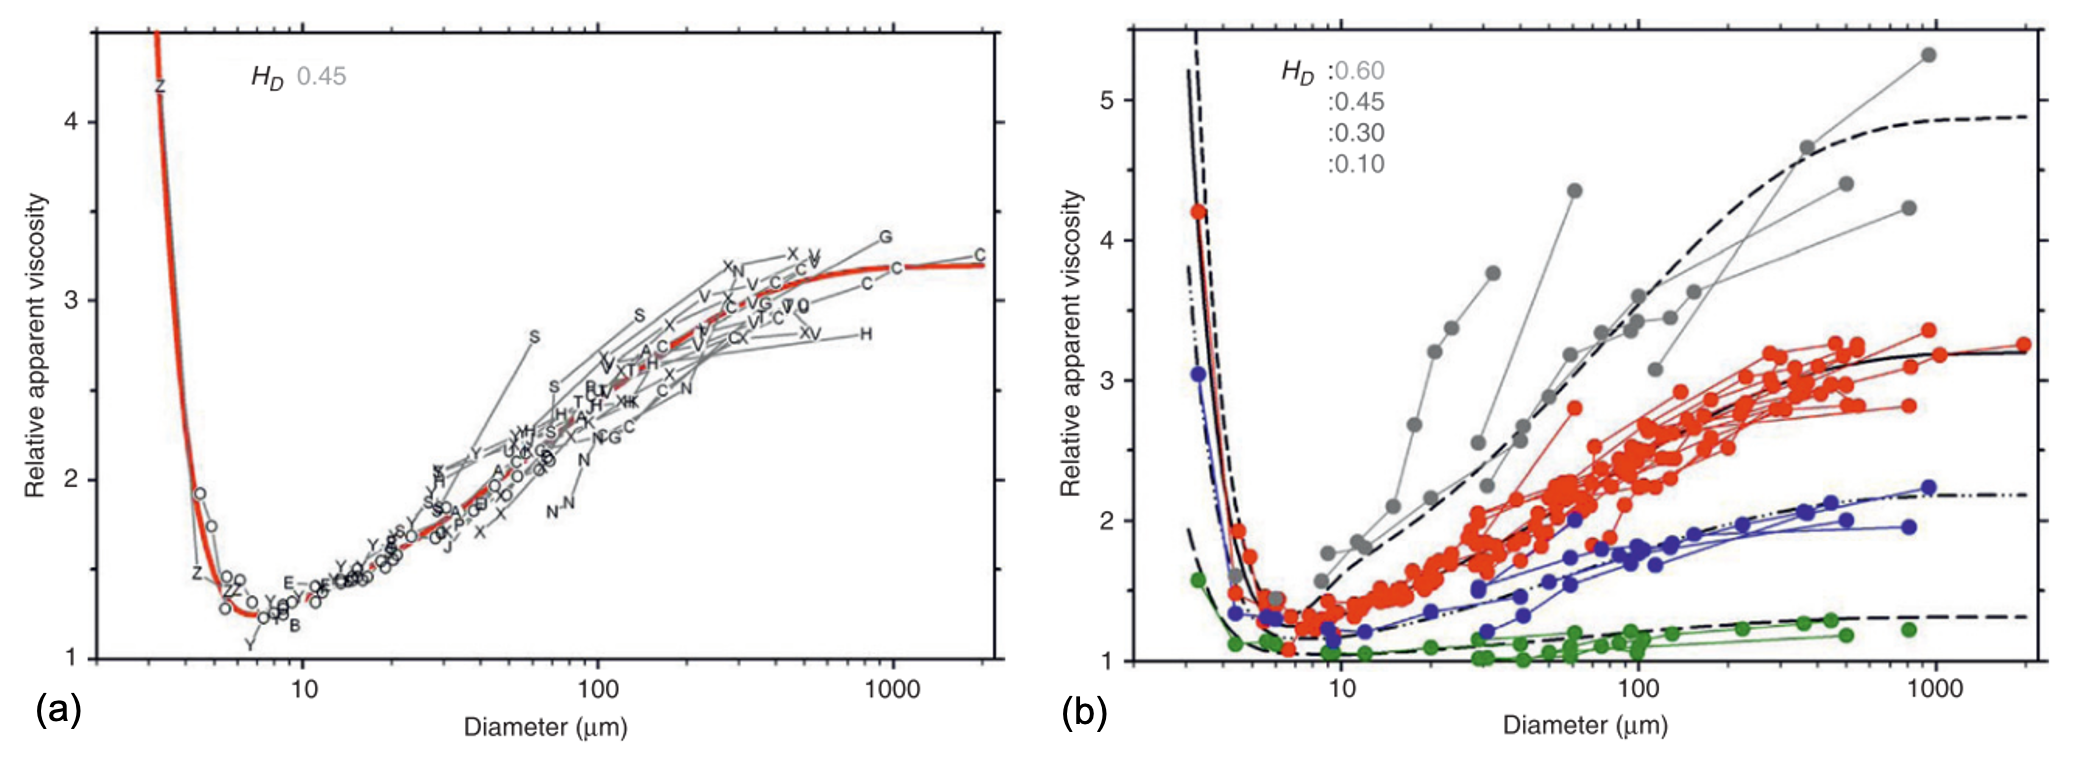
\includegraphics[width=1\textwidth]{images/ApparentViscosity.png}
\caption{\textit{An illustration of all experimental data including empirical lines based on results of parametric fittings. (a) represents the relative apparent viscosity expressed as a function of tube diameter at a discharge haematocrit of 45\%. (b) represents a collection of experimental data and approximations for different levels of discharge haematocrit. H$_{D}$: 0.6 (grey); H$_{D}$: 0.45 (red); H$_{D}$: 0.3 (blue); H$_{D}$: 0.1 (green)} \label{ApparentViscosity}}
\end{figure}

\noindent A comprehensive collection of all the experimental and theoretical results was put together into a graph (see Figure \ref{ApparentViscosity}) by Pries et al.\cite{Pries1992BloodHematocrit, BloodFlowSecomb} The results show that between 5$-$7 $\mu$m, apparent viscosity will reach its minimum before increasing further with decreasing diameter as this also applies to different haematocrit levels.\cite{Pries1992BloodHematocrit} Furthermore, it is expected that the apparent viscosity will increase with the increase of discharge haematocrit at any given diameter. However, between 5$-$7 $\mu$m, it was observed that even at higher haematocrit levels, the relative apparent viscosity remains below 1.5. This suggests that within this range, the presence of RBCs does not have much effect on the flow resistance on glass tubes. \\


\noindent Another important note is that according to these results in Figure \ref{ApparentViscosity}, the apparent viscosity of blood in living micro-vessels tend to be greater than its value in glass tubes with the same diameter. This is primarily due to the existence of endothelial surface layer (ESL) which impedes plasma flow and disrupts the flow of plasma and RBC along the micro-vessel.\cite{Pries2000TheLayer} Therefore, the flow resistance across micro-vessels observed in \textit{in vivo} studies are generally higher compared to that in capillary glass tubes in \textit{in vitro} studies. 

\subsection{Current Challenges in Reduced-Order Models}
\label{CurrentChallenges}
\noindent Over the years as the development of computational techniques have improved significantly, a plethora of computational studies\cite{Noguchi14159, DoddiSaiK2009Tcmo, Freund2014, Balogh2017DirectNetworks, 2020Charles, YAN199117, Possenti2019, EndenG1994ANSo, MehrabadiMarmar2015ACMf, VahidkhahKoohyar2014PDiT, HariprasadSecomb2014, Zhou2021EmergentBifurcations} have been conducted to elucidate and analyse the haemodynamics of blood flow in microvascular networks. To overcome the limitations of 2D systems, numerous 3D models emerged over recent years (E.g. immersed-boundary-lattice-Boltzmann model) to provide a reliable quantitative description of the microscopic behaviour of RBCs in micro- circulations.\cite{KrugerTimm2012Csso} However, conducting these studies required a lot of computational expense (i.e. GPU power) which hinders researchers to simulate RBC flows in large computational domains due to computational tractability limitations. Therefore, a great number of reduced-order models (ROM) were introduced to simplify the mathematical calculations in a computationally efficient manner and to overcome this limitation.\cite{A.R.Pries2005Mbvi, Romain2020, Bernabeu2020AbnormalOxygenation, Gould2015HematocritNetworks, PRIES198981, PriesAR1994RtBF} The main objective for ROMs is to quantitatively analyse and predict haemodynamic quantities with satisfactory accuracy in complex microvascular networks. \\

\noindent The validity of these ROMs is often restricted to a limited range due to a few conventional assumptions that are only applicable to certain conditions such as Poiseuille's Law. One example is from Pries's Phase Separation Model (PSM)\cite{A.R.Pries2005Mbvi, PriesAR1990BFiM, PRIES198981} which has the assumption of symmetrical haematocrit distribution in the feeding vessel. This assumption is usually invalid for actual micro-vessels given that the RBC distribution in these vessels was often observed to be asymmetric.\cite{2020Charles, Balogh2017DirectNetworks, Barber2011SimulatedPartitioning, Roman2016} Furthermore, most of these well-established ROMs are derived from experiments under certain assumptions and do not entirely quantify the true representation of the physiological phenomena associated with the motion of RBCs in complex microvascular networks. One example would be Pries's Viscosity Models (\textit{in vivo}\cite{PriesAR1994RtBF} and \textit{in vitro}\cite{Pries1992BloodHematocrit}) which are derived from experimental. This limits the capability of predicting the blood flow behaviour or mechanism that governs the radial distribution of RBCs in micro-vessels across the network at different scales. Therefore, further progress is required to better understand the fundamentals of the physical mechanisms in RBC flux partitioning. This will allow us to achieve reliable predictions of the physiological blood flow behaviours in both micro-circulation without simulating the motion of every individual RBC in large-scale numerical simulations. 

\subsection{Research Gaps in Literature}
\label{MissingGaps}
\noindent Following up with recent studies, only simulations of 2D simplified geometries or idealised 3D microvascular networks instead of realistic blood topology were used to analyse the physical mechanisms occurring in micro-circulations.\cite{Noguchi14159, DoddiSaiK2009Tcmo, Balogh2017DirectNetworks, 2020Charles, YAN199117, Possenti2019, EndenG1994ANSo, MehrabadiMarmar2015ACMf, VahidkhahKoohyar2014PDiT, HariprasadSecomb2014, Zhou2021EmergentBifurcations} This restricts the full potential of identifying or demonstrating certain fundamental effects in complex microvascular networks due to certain limitations. One example would be simulating 2D systems with only 1 particle as it will neglect the effects of cell-to-cell interactions and these 2D models are not able to accurately replicate the data from realistic 3D systems.\cite{PhysRevE.86.056308} Furthermore, for 2D systems, it is often assumed that there is no overlap in cell position along with uniform and independently distributed arrival times.\cite{Balogh2017DirectNetworks} This is not true for 3D complex network geometries as the RBCs travelling along the micro-vessels tend to form clusters due to the heterogeneity in their shape, size and deformability.\cite{gaehtgens1980motion} \\

\noindent The majority of the simulations consider the RBC properties of a normal healthy cell and no other suspended particles such as white blood cells (WBC) or platelets were considered in blood.\cite{Balogh2017DirectNetworks, 2020Charles, Balogh2018} The presence of WBCs or platelets are very likely to affect the RBC partitioning behaviours across the microvascular networks due to their important biological functions and cellular interactions. Also, based on the physical perspectives, considerations of including more biophysical properties of the RBCs (E.g. viscosity of RBCs and its membrane) will bridge us closer to simulate the actual blood flow behaviours in micro-circulation under physiological conditions. This also applies to the deformation and regulation of blood vessels in the simulated 3D complex networks. Therefore, this would allow us to attain more reliable results from the investigations of micro-circulatory blood flow and a deeper understanding of the hydrodynamic interactions of RBCs in blood flow. Last but not least, it will also significantly advance the wider biomedical and biophysical applications such as optimising micro-fluidic devices. 


%----------------------------------------------------------------------------------------
%	MATERIALS AND METHODS SECTION
%----------------------------------------------------------------------------------------
\newpage
\section{Materials \& Methods}
\noindent For this research project, the computer simulations were conducted by Qi Zhou\cite{2020Charles} while all of the data extraction and analyses are entirely my own work. The Materials \& Methods section explains how the simulation data was generated in Section \ref{GenerationOfSimulationData} and highlights what are the measured and calculated parameters gathered from the simulation data in Section \ref{Post_Processing}. Section \ref{Reduced_Order_Models} covers the relevant well-known reduced-order models for data analysis and comparison with simulation data. All in all, this section is dedicated to introducing all of the measurement methods and data processing involved in data analysis. 


\bigskip

\subsection{Introduction of Simulation Data}
\label{GenerationOfSimulationData}
\noindent First and foremost, all of the simulations for the whole-plexus network were conduct by Qi Zhou\cite{2020Charles} under the assumption that blood can be considered as a suspension of deformable RBC particles in a continuous plasma phase. The binary image of Col.IV mask of mouse retinal vasculature was used to reconstruct the entire 3D micro-vascular network using a computational tool developed by Bernabeu et al. called \textit{PolNet}.\cite{bernabeu2018polnet} Next, a non-Newtonian Carreau-Yasuda (NNCY) model\cite{Bernabeu2014} was used for the whole-plexus simulation of blood flow before conducting subsequent simulations of cellular blood flow in the selected region of interests (ROIs) from the capillary bed of the whole-plexus network. Afterwards, boundary conditions (e.g. inlet/outlet of blood flow and pressure) from the NNCY simulation are extracted to initiate plasma flow simulations and perfuse RBCs continuously at a constant haematocrit of 20\% from all inlets of the selected ROIs. \\


\noindent The RBC model developed by Timm Kr\"{u}ger\cite{KrugerTimm2012Csso} was used to model the RBCs as a deformable capsule with the hyper-elastic membrane of negligible thickness containing a viscous fluid called cytoplasm which consists of haemoglobin. This replicates the hyper-elastic behaviour of the RBC membrane in shear where total shear stress is the sum of all the viscous and elastic contributions. These simulation results were validated against \textit{in vivo} single-cell velocimetry data from Joseph et al.\cite{JosephAby2019Isbf} and Guevara-Torres et al.\cite{Guevara-Torres2016} which showed good agreement with existing experimental results. \\


\noindent As a result, these sets of simulation data (i.e plasma$+$RBC and plasma-only) were now collected to extract relevant data sets and conduct a few data analysis. The relevant data points (e.g. flow rates, pressure drops, branch diameter etc.) were extracted to find the distinct correlations that can describe the behaviours of RBCs distribution in complex microvascular networks. Moreover, several contributing factors to the blood flow behaviour in microvascular networks were also identified to quantitatively describe how well certain reduced-order models are with the simulation data such as apparent viscosity and RBC flux ratio. \\


\noindent The following points below are some of the key notes and assumptions made: 
\begin{itemize}
    \item Circular and smooth interior surface of blood vessel
    \item Blood flow consists of only normal healthy RBCs and plasma
    \item Since blood flow is assumed as a homogeneous shear-thinning fluid, Poiseuille's Law was used to evaluate the apparent viscosity of blood flow from simulation data. 
    \item Both viscosities of cytoplasm (fluid inside RBC) and plasma were modelled using the viscosity of plasma
    \item Physiological ocular perfusion pressure of 55 mmHg was used for the current simulation based on the research findings from Bernabeu et al.\cite{Bernabeu2014} 
    % \item RBCs centre of mass do not follow underlying fluid streamlines
    % \item Blood flow in the network does not follow Poiseuille's Law and is in the Stokes flow regime where Reynolds number is nearly zero, so inertial forces do not play a significant role.
\end{itemize}

% State why and explain you made those assumptions for each point in the bullet points above. % 

% \noindent Endothelial Surface Layer (ESL) is a single cell layer that forms the surrounding layers of the blood-vessel wall where the simulation data does not take this into account given that it was assumed that the ESL is not important for now. Therefore, the interior surface of blood vessel is considered smooth. White Blood Cells are also not considered. Furthermore, we assume the geometry of the blood flow network does not change and red blood cells' properties do not change. This means that we are only focusing on healthy blood flow. \\ 

\subsection{Post-Processing of Simulation Data}
\label{Post_Processing}
\noindent All of the haematocrits reported are discharged haematocrits, H$_{D}$, and it is calculated as the ratio of RBC flux to blood flow rate (Equation \ref{HaematocritEqn}) in each selected branch across the microvascular network. The volumetric blood flow is determined by integrating the blood velocity with respect to the cross- sectional area of the branch normal to the direction of blood flow. $Q_{rbc}$ represents the volumetric flow rate of RBCs while $Q_{blood}$ represents the volumetric flow rate of blood.

\begin{eqnarray}
\label{HaematocritEqn}
\begin{aligned}
H_{D} & = \frac{Q_{rbc}}{Q_{blood}}
\end{aligned}
\end{eqnarray}

\bigskip

\noindent The volumetric flow rate of RBC is calculated by counting the number of RBCs ($N$) crossing the same plane normal to the direction of blood flow over a given period of time, $\Delta t$. In order to satisfy mass conservation, the counting procedure is conducted when the total number of RBCs in the simulated network has become quasi-constant. Hence, given that the volume of an RBC is known (V$_{rbc}$ $=$ 100 $\mu$m$^{3}$), we can then calculate the RBC flow rate using Equation \ref{RBCflowrateEqn} below. 

\begin{eqnarray}
\label{RBCflowrateEqn}
\begin{aligned}
Q_{rbc} & = \frac{N \cdot V_{rbc}}{\Delta t}
\end{aligned}
\end{eqnarray}

\bigskip

\noindent The flow resistance ($R$) is evaluated from simulation data using the left-hand side (LHS) of the Hagen-Poiseuille's Equation\cite{PoiseuilleLaw} (Equation \ref{HagenPoiseuilleEqn1}) where direct measurements of blood flow rate ($Q_{blood}$) and pressure drop ($\Delta$P) for each branch are obtained via ParaView and Python. $\Delta$P is calculated by taking the difference between measured pressures at the start and endpoints of each branch. 

\begin{eqnarray}
\label{HagenPoiseuilleEqn1}
\begin{aligned}
R & = \frac{\Delta P}{Q} = \frac{128L\mu_{app}}{\pi D^{4}}
\end{aligned}
\end{eqnarray}

\bigskip

\begin{figure}[H]
\centering
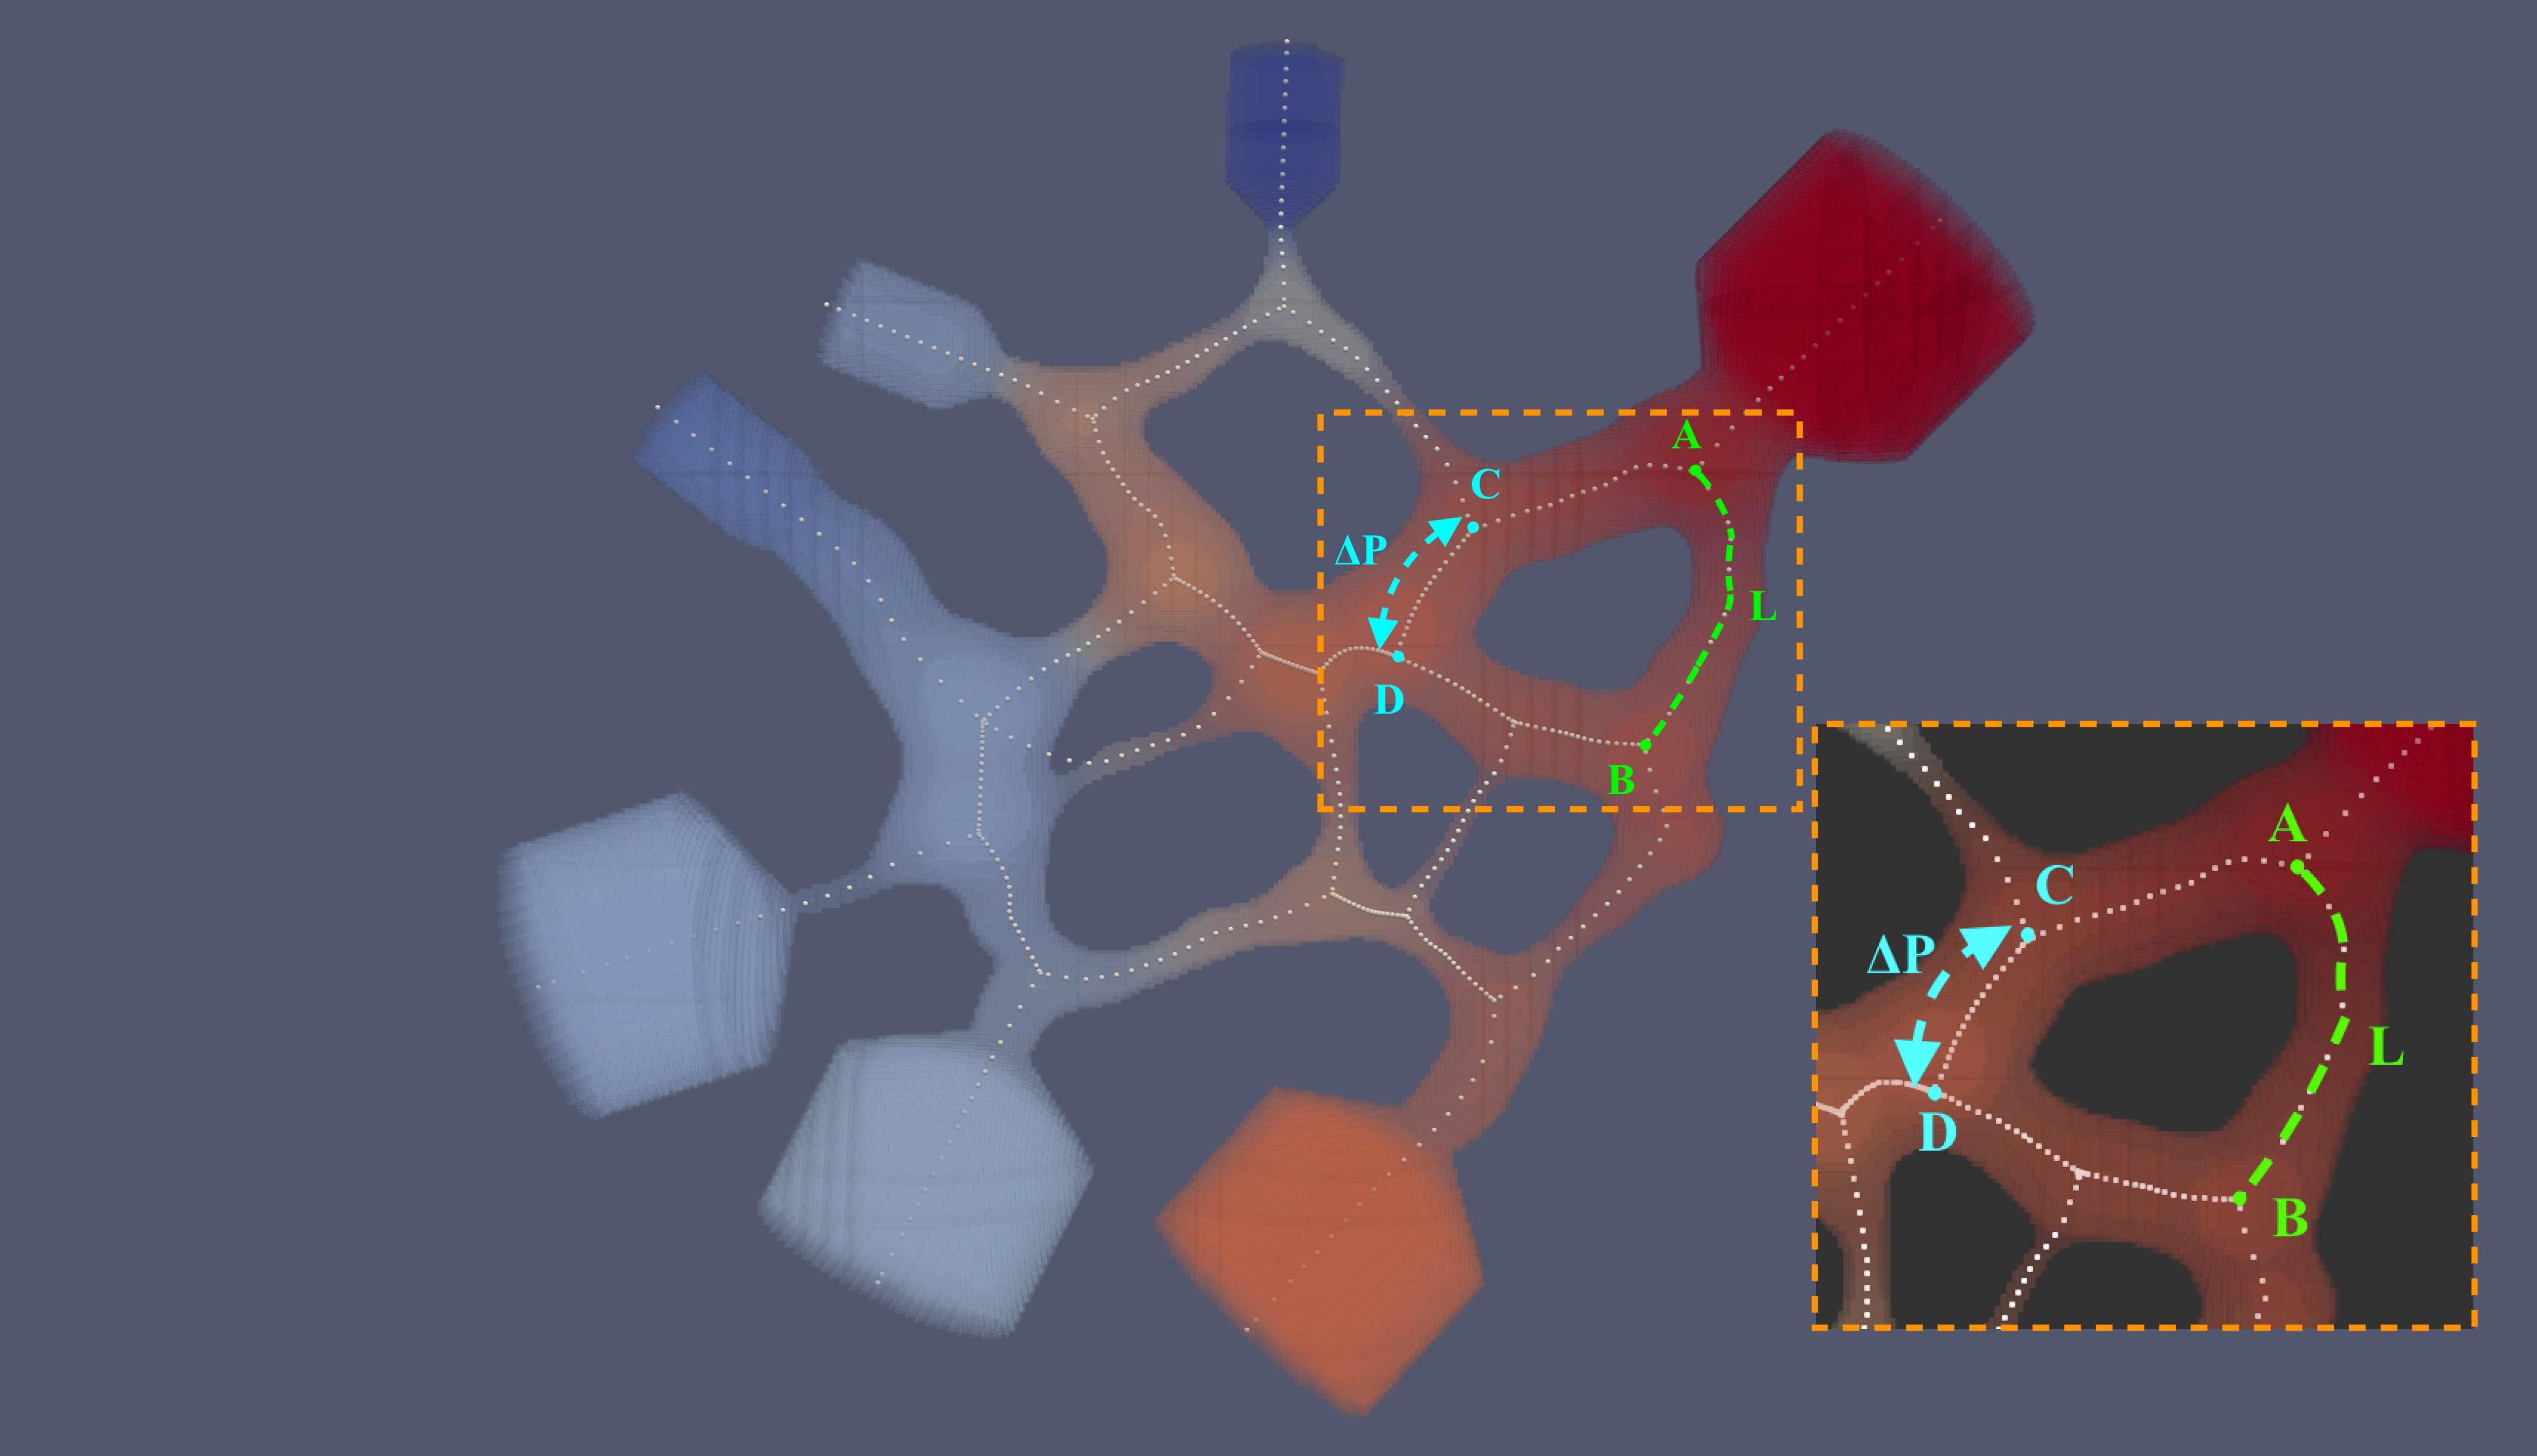
\includegraphics[width=1\textwidth]{images/ROI3-Geometry.png}
\caption{\textit{A complex micro-vascular network with an illustration of the measurement methods for pressure drop across the branch and branch length.} \label{measurementmethods}}
\end{figure}

\noindent Morphological variables such as the geometric diameter (D$_{G}$) and branch length ($L$) are measured as well based on the ROI geometries. D$_{G}$ is calculated by averaging all of the diameter measurements within a given vessel segment. Whereas for $L$, the distance between two points within a vessel is first measured before adding up all of the measured distances in the given vessel to obtain the magnitude of the branch length. In addition to this, the hydrodynamic diameter (D$_{H}$) of each branch is calculated using the Hagen-Poiseuille's Equation with the plasma-only simulation data. An illustration of the measurement methods is shown in Figure \ref{measurementmethods}. \\

\noindent Although the viscosity of blood flowing through micro-vessels is usually not constant, a simplified approach is used to obtain the apparent viscosity of blood (i.e. plasma+RBC) from simulation data. This is achieved by rearranging Equation \ref{HagenPoiseuilleEqn1} to Equation \ref{HagenPoiseuilleEqn2}. Therefore, it also allows us to conveniently analyse the rheological effects associated with RBCs in micro-vessels from simulation data. The relative apparent viscosity is defined as $\mu_{rel} = \mu_{app}/\mu_{p}$, where $\mu_{p}$ is the viscosity of suspending medium (i.e. plasma). A comparison is also made between the evaluated apparent viscosity values based on either geometric (D$_{G}$) or hydrodynamic (D$_{H}$) diameters in order to determine which is the preferable input parameter for apparent viscosity estimations. 


\begin{eqnarray}
\label{HagenPoiseuilleEqn2}
\begin{aligned}
\mu_{app} & = \frac{\pi}{128} \cdot \frac{\Delta PD^{4}}{LQ}
\end{aligned}
\end{eqnarray}

\bigskip

\noindent Since one of the most distinguished characteristics of micro-circulatory blood flow is the disproportionate partitioning of RBCs at vascular diverging bifurcations, the time-averaged behaviours of RBC partitioning are considered in the data analysis. Based on the studies from Pries et al.\cite{PRIES198981} and Balogh and Bagchi\cite{Balogh2018}, the ratio of blood flow rates (Q$^{*}_{blood}$) and RBC flux ratio (Q$^{*}_{rbc}$) between a child branch and the parent branch of each bifurcation are calculated using Equations \ref{Qratio1} and \ref{Qratio2} respectively as shown below.

\begin{eqnarray}
\label{Qratio1}
\begin{aligned}
Q^{*}_{blood} & = \frac{Q_{blood,CB}}{Q_{blood,PB}} 
\end{aligned}
\end{eqnarray}

\begin{eqnarray}
\label{Qratio2}
\begin{aligned}
Q^{*}_{rbc} & = \frac{Q_{rbc,CB}}{Q_{rbc,PB}} 
\end{aligned}
\end{eqnarray}
\bigskip

\subsection{Reduced-Order Models}
\label{Reduced_Order_Models}
\subsubsection{Pries's Phase Separation Model}
\noindent The Phase Separation Model (PSM) consists of a list of empirical equations that were derived from experimental observations of arteriolar bifurcations in a rat mesentery and was developed by Pries et al.\cite{A.R.Pries2005Mbvi, PriesAR1990BFiM} through theoretical modelling. The PSM has established a flow-mediated mechanism that could quantitatively predict the amount of RBC fluxes in the child branches of diverging bifurcations within a network of micro-vessels. The fractional RBC flux (\textit{FQ$_{E}$}) in each child branch is given as a function of the fractional blood flow (\textit{FQ$_{B}$}) entering that child branch:

\begin{eqnarray}
\label{Pries_equation1}
\begin{aligned}
logit FQ_{E} & = A + B \thinspace logit \frac{(FQ_{B} - X_{0})}{(1 - 2X_{0})}
\end{aligned}
\end{eqnarray}

\bigskip

\noindent where $logit$ $x$ $=$ ln($\frac{x}{1-x}$) and X$_{0}$ < FQ$_{B}$ < 1 $-$ X$_{0}$. The fitting parameters $A$, $B$ and $X_{0}$ were obtained via linear regression analysis. $A$ represents the size difference of both child branches, $B$ describes the shape of the haematocrit profile in the parent branch and $X_{0}$ is associated with the cell-free layer thickness near the inner branch walls. \\

\begin{eqnarray}
\label{Pries_equationA}
\begin{aligned}
A & = -13.29\bigg[\bigg(\frac{D_{\alpha}^{2}}{D_{\beta}^{2} -1}\bigg) \bigg/ \bigg(\frac{D_{\alpha}^{2}}{D_{\beta}^{2} +1}\bigg)\bigg]\bigg[\frac{(1 - H_{D,PB})}{D_{PB}}\bigg]
\end{aligned}
\end{eqnarray}

\begin{eqnarray}
\label{Pries_equationB}
\begin{aligned}
B & = 1 + 6.98\bigg[\frac{1 - H_{D,PB}}{D_{PB}}\bigg]
\end{aligned}
\end{eqnarray}

\begin{eqnarray}
\label{Pries_equationX}
\begin{aligned}
X_{0} & = 0.964\bigg[\frac{1-H_{D,PB}}{D_{PB}}\bigg]
\end{aligned}
\end{eqnarray}

\bigskip

\noindent where $D_{\alpha}$, $D_{\beta}$, and $D_{PB}$ are the diameters of two child branches and the parent branch respectively while $H_{D,PB}$ represents the discharge haematocrit in the parent branch. The simulation data in the form of $Q^{*}_{rbc}$ against $Q^{*}_{blood}$ are plotted with the empirical curves for each bifurcation in order to observe the deviations between simulation data and the empirical predictions from PSM. \\

\noindent The following points are some key notes for Pries's Phase Separation Model:\cite{A.R.Pries2005Mbvi, PriesAR1990BFiM, PRIES198981}
\begin{itemize}
    \item Assumes haematocrit profile in the parent branch of a diverging bifurcation is symmetrical
    % \item Planar flow separation surface between the fluid spaces entering the child branches (A = 0)
    \item Velocity profile in the parent branch was assumed to be parabolic
    \item Under dilute/semi-dilute suspensions, the RBCs are assumed to follow the fluid streamlines (i.e. plasma) in the vicinity of the bifurcation
    \item Empirical model does not take into account the bifurcation angle as it was proven to be of minor importance. 
\end{itemize}

% Put the key notes in a paragraph instead of bullet points % 
\bigskip

\subsubsection{Pries's Viscosity Model (\textit{in vitro})}
\noindent Based on original publications by Fahraeus and Lindqvist\cite{Fahrus1931THETUBES}, it has been reported that the tube diameters affect the relative apparent viscosity of blood in tube flow. However, the dependence of blood viscosity on haematocrit in the different diameter tubes are required as well in order to develop hydrodynamic models of blood flow through micro-circulation. Based on \textit{in vitro} experiments using glass capillary tubes, a set of empirical fitting equations were derived by Pries\cite{Pries1992BloodHematocrit} to achieve a quantitative description of the relative apparent viscosity as a function of tube diameter and discharge haematocrit as shown in Equation \ref{viscosity_equation4}:

\begin{eqnarray}
\label{viscosity_equation4}
\begin{aligned}
\mu_{rel} & = \bigg[1 + (\mu_{45} - 1) \frac{(1-H_{D})^{C} - 1}{(1-0.45)^{C} - 1} \bigg]
\end{aligned}
\end{eqnarray}

\bigskip

\noindent where $\mu_{45}$ is the relative apparent blood viscosity for a fixed discharge haematocrit of 0.45 based on Equation \ref{viscosity_equation5} and $C$ represents the shape of the viscosity dependence on haematocrit. 

\begin{eqnarray}
\label{viscosity_equation5}
\begin{aligned}
\mu_{45} & = 220 e^{-1.3D} + 3.2 - 2.44e^{-0.06D^{0.645}}
\end{aligned}
\end{eqnarray}

\begin{eqnarray}
\label{viscosity_equation3}
\begin{aligned}
C & = (0.8 + e^{-0.075D}) \cdot \bigg(-1 + \frac{1}{1 + 10^{-11}D^{12}} \bigg) + \frac{1}{1 + 10^{-11}D^{12}}
\end{aligned}
\end{eqnarray}

\bigskip
\newpage

\noindent The following points are some key notes for Pries's Viscosity Model (\textit{in vitro}):\cite{Pries1992BloodHematocrit}
\begin{itemize}
    \item Long, straight and smooth glass capillary tubes were used (tube length $\in$ [6, 11]mm and tube diameter $\in$ [9, 40]$\mu$m)
    \item It is assumed that the volume concentration of blood for both inlet and outlet of the capillary tube remain constant (discharge haematocrit equals to feed haematocrit)
    \item Presence of phase separation effects are absent in the studied capillary tubes
\end{itemize}

% Put the key notes in a paragraph instead of bullet points % 
\bigskip

\subsubsection{Pries's Viscosity Model (\textit{in vivo})}
\noindent The apparent viscosity of blood in micro-vessels can be different from bulk viscosity as the non-continuum effects become more prominent especially in microvascular networks (micro-scale). Therefore, an approach for quantifying the effects of blood flow properties on the flow resistance of a micro-vessel is developed by Pries et al.\cite{PriesAR1994RtBF} using the vessel segments of terminal micro-circulatory networks in the rat mesentery. Based on \textit{in vivo} experimental results, an empirical relationship was derived to describe the relative apparent viscosity of blood as a function of branch diameter and haematocrit as shown below in Equation \ref{viscosity_equation1}:

\begin{eqnarray}
\label{viscosity_equation1}
\begin{aligned}
\mu_{rel} & = \bigg[1 + (\mu_{45} - 1) \cdot \frac{(1-H_{D})^{C} - 1}{(1-0.45)^{C} - 1} \cdot \bigg(\frac{D}{D - 1.1}\bigg)^{2} \bigg] \cdot \bigg(\frac{D}{D - 1.1}\bigg)^{2}
\end{aligned}
\end{eqnarray}

\bigskip

\noindent where $\mu_{45}$ is the relative apparent blood viscosity for a fixed discharge haematocrit of 0.45 based on Equation \ref{viscosity_equation2} and $D$ refers to the luminal vessel diameter. $C$ is the same parameter used in the \textit{in vitro} formulation of Pries's Viscosity Model as shown in Equation \ref{viscosity_equation3}.

\begin{eqnarray}
\label{viscosity_equation2}
\begin{aligned}
\mu_{45} & = 6 e^{-0.085D} + 3.2 - 2.44e^{-0.06D^{0.645}}
\end{aligned}
\end{eqnarray}

\bigskip

\noindent The difference between the empirical equations derived from \textit{in vitro} and \textit{in vivo} experiments is primarily due to the relatively short and irregularly shaped vessels in the micro-vascular networks compared to the long, straight and smooth capillary tubes. This irregularity affects the hydrodynamic diameter of the vessel which is why the Equation \ref{viscosity_equation4} was modified to Equation \ref{viscosity_equation1} by including a diameter-dependent term with its optimised parameters. \\

\noindent The following points are some key notes for Pries's Viscosity Model (\textit{in vivo}):\cite{PriesAR1994RtBF}
\begin{itemize}
    \item Average length and diameter of vessel segments in the rat mesentery are of the order of 350 $\mu$m and 8.7 $\mu$m respectively
    \item Presence of endothelial surface layer is considered at the inner wall of micro-vessels
    \item Irregular inner vessels contour across the micro-circulation network and disrupts the distribution of RBCs flowing through the vessels which may give rise to additional energy dissipation. 
\end{itemize}


%----------------------------------------------------------------------------------------
%	RESULTS AND DISCUSSIONS SECTION
%----------------------------------------------------------------------------------------
\newpage
\section{Data Analysis with Discussions}
\noindent In this section, all of the evaluated results obtained from data analysis are explained with discussions where several key findings are highlighted. Section \ref{Vessel_Bifurcation_Selection} summarises the ranges of branch diameter and length found within the total number of eligible vessels and bifurcation selected for data analysis. In Section \ref{RBC_Enrichment_Depletion}, prediction of RBC enrichment or depletion branches with different variables is identified and discussed, followed by demonstrating the presence of plasma skimming effects within the studied networks in Section \ref{Plasma_Skimming_Effects}. The evaluated deviations between empirical predictions against simulation data for apparent viscosity is analysed in Section \ref{BreakdownInPriesViscosityModels} and subsequently validating the presence of F{\aa}hr{\ae}us-Lindqvist effect in Section \ref{Fahraeus_Lindqvist_Effect}. The influence of branch length and distance ratio onto apparent viscosity is demonstrated in Section \ref{BranchLength_DistanceRatio} which leads to identifying the contributing factors to asymmetric RBC distribution in Section \ref{ContributingFactorsTOAsymmetricRBCDistribution}. Finally, identified invalid data points are mentioned and discussed in Section \ref{InvalidDataPoints} with justifiable reasons. 

% the existence of certain haemodynamic effects and the importance of distance ratio 

% \noindent In this section, all of the evaluated results obtained from data analysis are explained with discussions where several key findings are highlighted. Both evaluated results and discussions are based on a curiosity-driven approach where each key finding leads directs the next investigation to discover new results and point out the key highlights. \\

% \noindent Section \ref{Vessel_Bifurcation_Selection} summarises the ranges of branch diameter and length found within the total number of eligible vessels and bifurcation selected for data analysis. In Section \ref{RBC_Enrichment_Depletion}, prediction of RBC enrichment or depletion branches with different variables is identified and discussed, followed by demonstrating the presence of plasma skimming effects within the studied networks in Section \ref{Plasma_Skimming_Effects}. The evaluated deviations between empirical predictions against simulation data for apparent viscosity is analysed in Section \ref{BreakdownInPriesViscosityModels} and subsequently validating the presence of F{\aa}hr{\ae}us-Lindqvist effect in Section \ref{Fahraeus_Lindqvist_Effect}. The influence of branch length and distance ratio onto apparent viscosity is demonstrated in Section \ref{BranchLength_DistanceRatio} which leads to identifying the contributing factors to asymmetric RBC distribution in Section \ref{ContributingFactorsTOAsymmetricRBCDistribution}. Finally, identified invalid data points are mentioned and discussed in Section \ref{InvalidDataPoints} with justifiable reasons. 

\bigskip

\subsection{Bifurcation \& Vessel Selection}
\label{Vessel_Bifurcation_Selection}
\noindent For the study of RBCs distribution in microvascular networks, three different regions of interest (ROIs) were selected with a specific focus on diverging bifurcations (i.e comprise of one parent branch and two downstream child branches) as shown in Figure \ref{ROIs}. To achieve an independent characterisation of the systematic RBC partitioning behaviours taking place in the studied networks, only branches from these diverging bifurcations are chosen for data analysis. Collectively, 23 diverging bifurcations and 57 independent branches (excluding 12 identical branches) were selected from the three ROIs with diameters ranging from 2.3 $\mu$m to 23 $\mu$m and branch lengths ranging from 6.5 $\mu$m to 60.6 $\mu$m. Furthermore, the system haematocrit was found to be around 21.8\%. (see Figure \ref{SystemHaematocrit} in Appendix \ref{SystemHaematocritInMicrovascularNetworks})

% ("average" discharge haematocrit in the whole network)

\subsection{Prediction of RBC Enrichment/Depletion}
\label{RBC_Enrichment_Depletion}
\noindent To determine whether the child branches across the network are either "RBC-enriched" or "RBC- depleted", Q$^{*}_{blood}$ and Q$^{*}_{rbc}$ were evaluated first before considering the sign and magnitude of $\Delta$Q$^{*}$ $=$ Q$^{*}_{rbc}$ $-$ Q$^{*}_{blood}$. (Refer back to Section \ref{Post_Processing} for definitions and equations of variables here. E.g. Q$^{*}_{blood}$) If the RBCs were distributed in proportional to the blood flow, it implies that $\Delta$Q$^{*}$ $=$ 0 which shows a linear relationship between Q$^{*}_{blood}$ and Q$^{*}_{rbc}$. For "RBC-enriched" branches, Q$^{*}_{rbc}$ > Q$^{*}_{blood}$ as this indicates that the child branch has more RBCs than linear allocation. Whereas when Q$^{*}_{rbc}$ < Q$^{*}_{blood}$, the child branch is referred to as an "RBC-depleted" branch given that the child branch has fewer RBCs than the linear hypothesis. \\


\noindent Based on the given simulation data, several branches were found without any presence of RBCs. This raises a critical question on what are the governing factors that could influence the blood flow in microvascular networks. Although it is natural to think that very narrow branches (smaller than the diameter of a human RBC) should restrict RBCs from passing through, several studies\cite{FreundJonathanB2013Tfor, Salehyar2017EffectsOS, LuHuijie2019Biso} have shown that highly deformable RBCs under physiological conditions allows them to pass through extremely confined branches with diameters even as small as 1$-$2 $\mu$m.


\subsubsection{Geometric \& Hydrodynamic Diameters}
\noindent For all of the child branches examined in this data analysis (46 in total, Figure \ref{DisproportionalityIndexDs}), it was observed that RBC depletion occurs throughout the entire range of both geometric and hydrodynamic branch diameters, whereas RBC enrichment occurs only when D$_{G}$ and D$_{H}$ are greater than 6.7 $\mu$m. In addition to this, one specific child branch with D$_{G}$ $\approx$ 10.5 $\mu$m (larger than the diameter of an RBC) had a disproportionality index of $-$0.21 which indicates a 21$\%$ reduction in RBC transit in that child branch. This shows that RBC depletion in the micro-vascular network cannot be purely based on geometric measurements of the network and hence, it is not a size-exclusion effect. Last but not least, for branch diameters between 6.7 $\mu$m and 14 $\mu$m, the branches have almost equivalent probabilities of being either enriched or depleted. Therefore, the branch diameters (D$_{G}$ and D$_{H}$) obtained from the given simulation data indicate that branch diameters alone do not differentiate the RBC enrichment or depletion apart as shown in Figure \ref{DisproportionalityIndexDs}. This also demonstrates that branch diameter is not the primary factor affecting RBC transits in microvascular networks. (Refer back to Section \ref{Post_Processing} for the methods of calculating D$_{G}$ and D$_{H}$)

\begin{figure}[H]
\centering
\begin{subfigure}{0.48 \textwidth}
    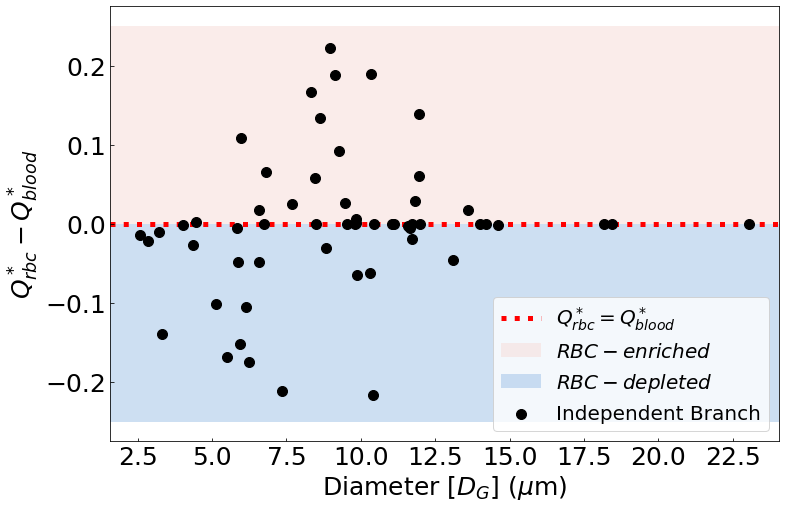
\includegraphics[width=1\textwidth]{images/DisproportionalityIndexDG.png}
    \caption{\textit{Average Geometric Diameters} \label{DisproportionalityIndexDG}}
\end{subfigure}
\hfill
\begin{subfigure}{0.48 \textwidth}
    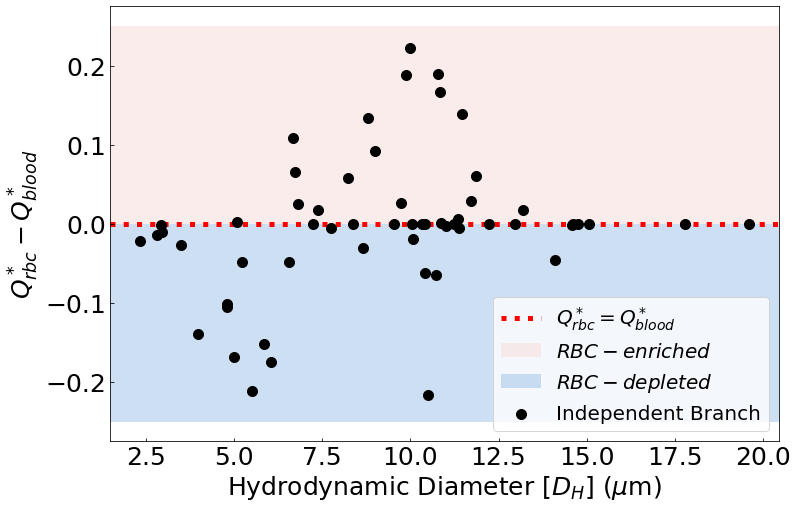
\includegraphics[width=1\textwidth]{images/DisproportionalityIndexDH.png}
    \caption{\textit{Evaluated Hydrodynamic Diameters} \label{DisproportionalityIndexDH}}
\end{subfigure}
\caption{\textit{Quantification of RBC enrichment and depletion in micro-vascular networks based on branch diameters. Q$^{*}_{blood}$ and Q$^{*}_{rbc}$ represent the normalised blood flow and RBC flux in a child branch relative to its parent branch in each bifurcation respectively. $\Delta$Q$^{*}$ $=$ Q$^{*}_{rbc}$ $-$ Q$^{*}_{blood}$ represents an index that describes the disproportionality of RBC partitioning where the sign of $\Delta$Q$^{*}$ indicates which branches are classified as "RBC-depleted" (negative $\Delta$Q$^{*}$, blue region) and "RBC-enriched" (positive $\Delta$Q$^{*}$, red region).} \label{DisproportionalityIndexDs}}
\end{figure}

\subsubsection{Discharge Haematocrit}
\begin{figure}[H]
\centering
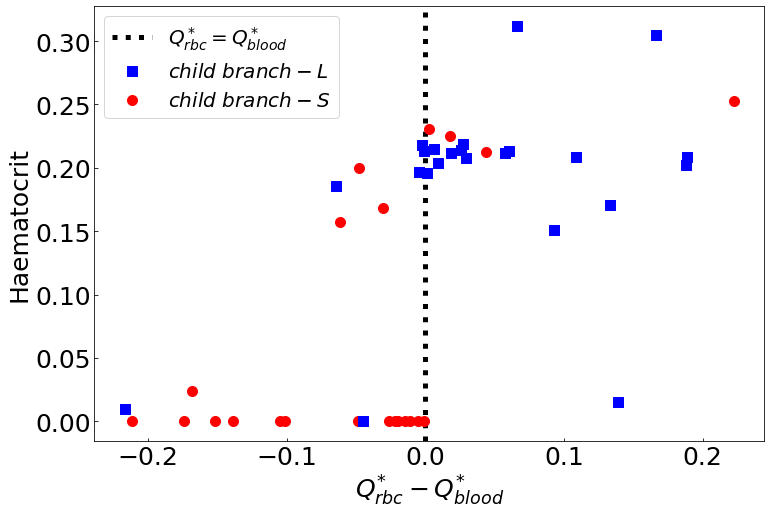
\includegraphics[width=0.65\textwidth]{images/DisproportionalityIndexHD.png}
\caption{\textit{Network level inspection of RBC enrichment (right-hand region) / RBC depletion (left-hand region) based on haematocrit. The "L"/"S" indicate the relatively larger (blue squares) / smaller (red circles) child branches in each of the investigated bifurcations across the networks respectively. The black dotted line represents Q$^{*}_{blood}$ $=$ Q$^{*}_{rbc}$.} \label{DisproportionalityIndexHD}}
\end{figure}

\noindent Meanwhile, discharge haematocrit (H$_{D}$) is another important factor for consideration to determine the effects of RBC transits across the microvascular networks. Based on Figure \ref{DisproportionalityIndexHD} above, it was observed that the majority of the close-to-zero haematocrit child branches are "RBC-depleted" although there are a few child branches spotted experiencing RBC depletion even with an average haematocrit of around 18\%. The range of H$_{D}$ in the RBC enrichment region except for one single outlier was found between 0.15 and 0.31. Last but not least, it is evident that the majority of the larger and smaller child branches are within the RBC enrichment and RBC depletion regions respectively. Therefore, in accordance with these findings, we can conclude that neither discharge haematocrit nor branch diameter alone is able to distinctively predict which branches are categorised as either "RBC-depleted" or "RBC-enriched". Furthermore, although the majority of the larger and smaller child branches lie within the RBC-enrichment and RBC-depletion regions respectively, there are still several anomalies that suggest that both the discharge haematocrit and branch diameter should be simultaneously considered instead. Kindly note that the context of "larger" and "smaller" (CB-L and CB-S) in the entire dissertation is a comparative notion between the two child branches in each bifurcation and not a measure of the absolute branch diameter. 



\subsection{Presence of Plasma Skimming Effect in microvascular network}
\label{Plasma_Skimming_Effects}
\noindent Considering that $\Delta$Q$^{*}$ $=$ Q$^{*}_{rbc}$ $-$ Q$^{*}_{blood}$ against either the discharge haematocrit or branch diameter alone could not differentiate the RBC-depletion zone from the RBC-enrichment zone, haemodynamic indicators like Q$^{*}_{blood}$ was examined instead. Excluding one single outlier from Figure \ref{DisproportionalityIndexQblood} below, we have noticed that the differentiation between RBC-depletion and RBC-enrichment for each child branch can be determined with the fractional blood flow Q$^{*}_{blood}$ in the given child branch. This observation features a potential haemodynamic mechanism that may exist in the microvascular networks based on simulation data. For this reason, the time-averaged behaviour of RBC partitioning was considered (as shown in Figure \ref{TimeAveragedRBCPartitioningBehaviours}) to assess for the presence of the Zweifach-Fung effect.\cite{SVANES1968210, FUNG197334} The results show that majority of the investigated child branches have classical partitioning behaviour while only a small number of those branches have reverse partitioning behaviour. Hence, this demonstrated the presence of the Zweifach-Fung effect which describes the heterogeneous partitioning behaviour of RBC suspension for both child branches in each selected bifurcation across the networks. 

\begin{figure}[H]
\centering
\begin{subfigure}{0.48 \textwidth}
    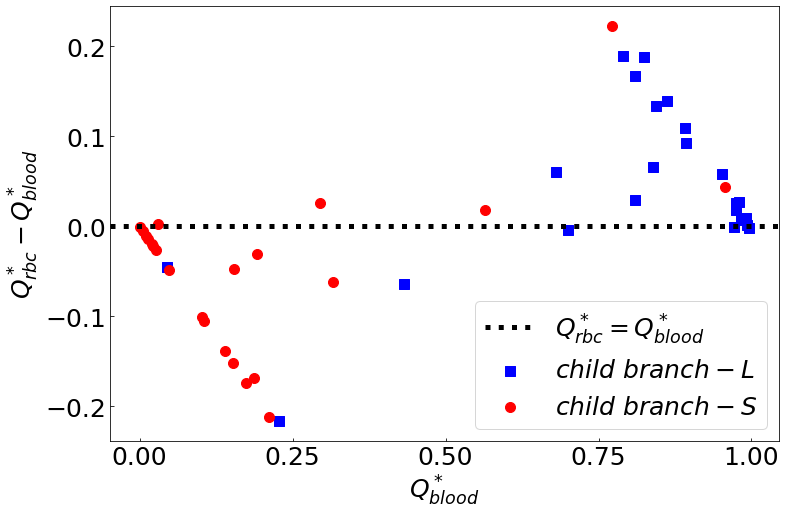
\includegraphics[width=1\textwidth]{images/DisproportionalityIndexQblood.png}
    \caption{\textit{Disproportionality Indices for all of the investigated child branches against normalised blood flow Q$^{*}$ across the networks} \label{DisproportionalityIndexQblood}}
\end{subfigure}
\hfill
\begin{subfigure}{0.48 \textwidth}
    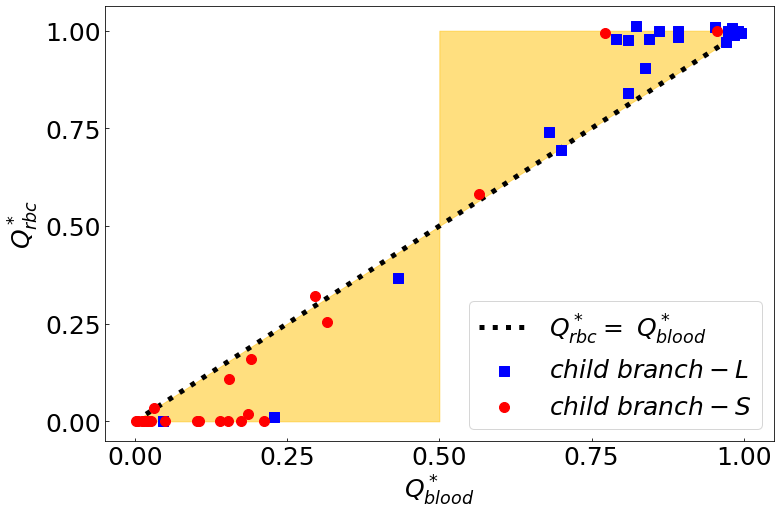
\includegraphics[width=1\textwidth]{images/TimeAveragedRBCPartitioningBehaviours.png}
    \caption{\textit{Time-averaged RBC Partitioning Behaviours found across the networks, Classical: 52 branches (yellow region) | Reverse: 5 branches (white region)} \label{TimeAveragedRBCPartitioningBehaviours}}
\end{subfigure}
\caption{\textit{Distinct correlation between $\Delta$Q$^{*}$ $=$ Q$^{*}_{rbc}$ $-$ Q$^{*}_{blood}$ and Q$^{*}_{blood}$ highlights a potential haemodynamic mechanism within the micro-vascular networks. Simulation data of Q$^{*}_{rbc}$ against Q$^{*}_{blood}$ distinguishes the different RBC partitioning behaviours occurring for the child branches within each bifurcation. The black dotted line represents a linear hypothesis for Q$^{*}_{blood}$ and Q$^{*}_{rbc}$ without the presence of plasma skimming.} \label{PlasmaSkimmingEffects}}
\end{figure}

\noindent In reference to these findings from simulation data, it does suggest to us the existence of plasma skimming effect occurring in the micro-vascular networks. For the purpose of validation, the simulation data at each diverging bifurcation was compared to the empirical predictions from the PSM model (Equations \ref{Pries_equation1}$-$\ref{Pries_equationX}).\cite{A.R.Pries2005Mbvi, PriesAR1990BFiM} The results indicated 17 out of 23 bifurcations show good agreement with predictions from PSM with errors of less than 5$\%$ (see Table \ref{ErrorsPSM} for complete error evaluation). An illustration of two exemplar bifurcations showing that the simulation data matched well with empirical predictions is presented in Figure \ref{DeviationsPSM}a$-$b. In the first bifurcation (Figure \ref{DeviationsPSM1}), both child branches have a substantial fraction of blood flow (approximately 30\% and 70\% in CB-S and CB-L respectively) with fractional RBC fluxes almost identical to PSM predictions. In the second bifurcation (Figure \ref{DeviationsPSM2}), the larger child branch has almost all of the RBCs (Q$^{*}_{rbc}$ $\approx$ 98\%) as it receives close to 90\% of the blood flow from the parent branch which leaves the smaller child branch with practically little blood flow and no RBCs. 

\begin{figure}[H]
\centering
\begin{subfigure}{0.48 \textwidth}
    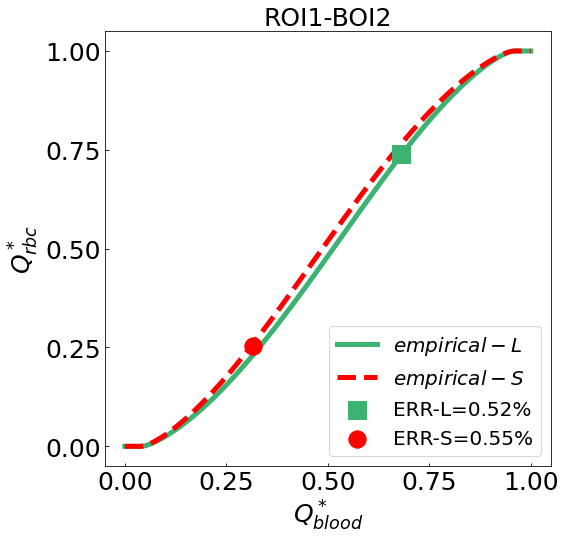
\includegraphics[width=0.92\textwidth]{images/DeviationsPSM1.png}
    \caption{\textit{Proportions of blood flow (Q$^{*}_{blood}$) in CB-L and CB-S are approximately 70\% and 30\% respectively} \label{DeviationsPSM1}}
\end{subfigure}
\hfill
\begin{subfigure}{0.48 \textwidth}
    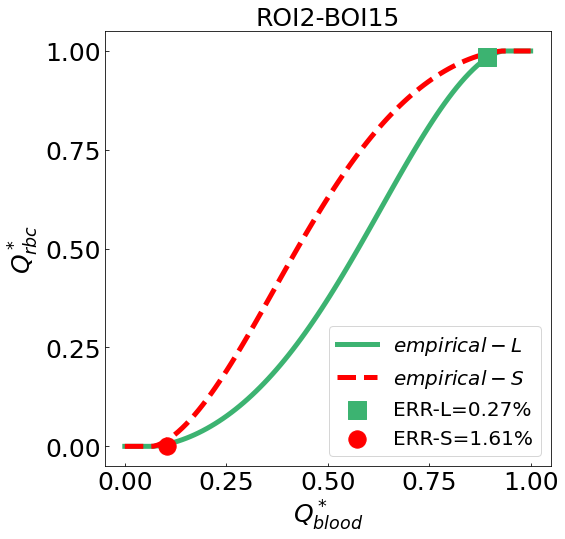
\includegraphics[width=0.92\textwidth]{images/DeviationsPSM2.png}
    \caption{\textit{Proportions of blood flow (Q$^{*}_{blood}$) in CB-L and CB-S are approximately 90\% and 10\% respectively} \label{DeviationsPSM2}}
\end{subfigure}
\hfill
\begin{subfigure}{0.48 \textwidth}
    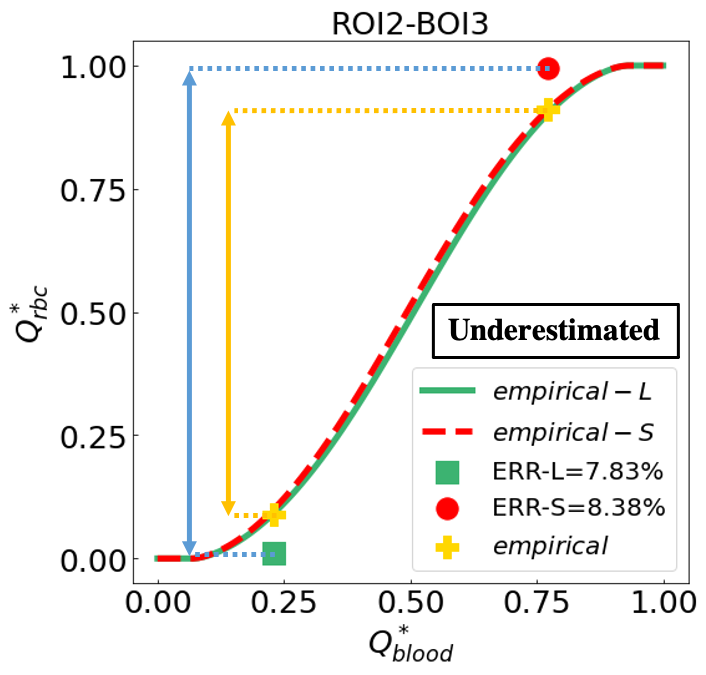
\includegraphics[width=0.92\textwidth]{images/DeviationsPSM3.png}
    \caption{\textit{PSM model slightly underestimated RBC flux comparison between the two child branches} \label{DeviationsPSM3}}
\end{subfigure}
\hfill
\begin{subfigure}{0.48 \textwidth}
    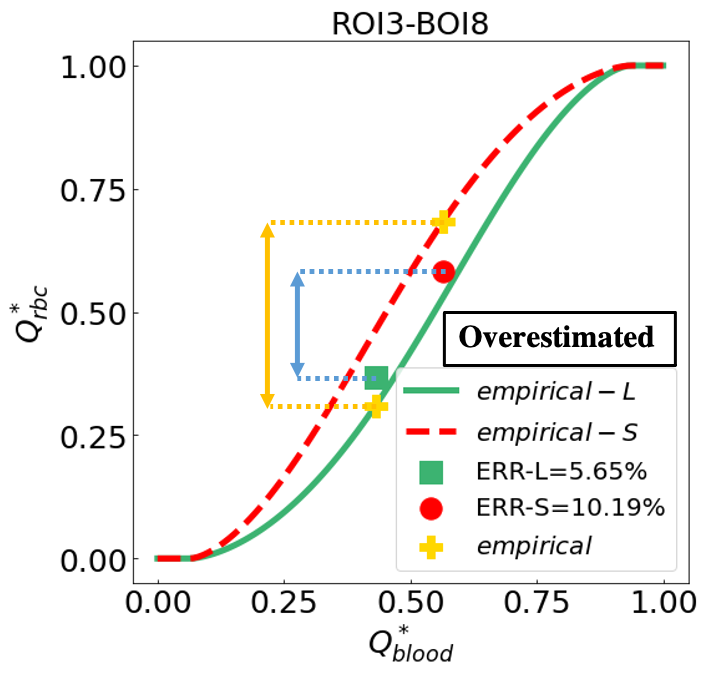
\includegraphics[width=0.92\textwidth]{images/DeviationsPSM4.png}
    \caption{\textit{PSM model considerably overestimated RBC flux comparison between the two child branches} \label{DeviationsPSM4}}
\end{subfigure}
\caption{\textit{Examples of good (a$-$b) and bad (c$-$d) matches of fractional RBC fluxes (Q$^{*}_{rbc}$) between simulation data (squares and circles) and the empirical predictions (solid lines and crosses) from Pries Phase Separation Model based on the given proportion of blood flows for both the "L" and "S" child branches in each selected bifurcation.} \label{DeviationsPSM}}
\end{figure}

\noindent For the remaining 6 of 23 bifurcations investigated, the simulated RBC fluxes have deviations of greater than 5\% against the PSM predictions, and two of such bifurcations are shown in Figure \ref{DeviationsPSM}c$-$d. The difference in RBC flux between the two child branches for the first bifurcation (Figure \ref{DeviationsPSM3}) marginally underestimated the PSM predictions while it is significantly overestimated for the second bifurcation (Figure \ref{DeviationsPSM4}). Such observations are found because of the asymmetric RBC distribution in the cross-sections of the parent branches which is opposed to the primary assumption of symmetrical haematocrit profile by the empirical model. Therefore, without the knowledge of the cross-sectional RBC distributions, it will be challenging to accurately predict the RBC perfusion in any given vascular network. \\

\noindent In consideration of the above findings, the Phase Separation Model developed by Pries et al.\cite{A.R.Pries2005Mbvi, PriesAR1990BFiM} attributed to the plasma skimming effect has appropriately described the RBC flux partitioning in 17 out of the 23 selected bifurcations. (see Figures \ref{DisproportionalityIndexQblood-ROI1}$-$\ref{DisproportionalityIndexQblood-ROI3} in the Appendix \ref{EvaluationOfSimulationDataVSPSM}) Therefore, this implies that the mechanism behind RBC enrichment/depletion within the studied networks is the plasma skimming effect. Also, this suggests that the RBC distribution within the micro-vascular network is flow-mediated instead of geometry-dominant.



\begin{table}[H]
\centering
\caption{\textit{Full evaluation of the deviations between simulation data and the empirical predictions from Pries Phase Separation Model. The "L"/"S" indicate the relatively larger and smaller child branches in each diverging bifurcation respectively.}
\label{ErrorsPSM}}
\scalebox{0.75}{
\begin{tabular}{*{11}{c}}
\dtoprule
\textbf{ROIs} & \textbf{CBs} & \textbf{BOI-2} & \textbf{BOI-7} & \textbf{BOI-9} & \textbf{BOI-10} & \textbf{BOI-11} & \textbf{BOI-13} & $-$ & $-$ & $-$ \\
\midrule[0.5pt]
\multirow{2}{*}{ROI-1} & CB-L & 0.52\% & 2.39\% & 0.68\% & 0.68\% & 0.0\% & 0.0\% & $-$ & $-$ & $-$ \\
& CB-S & 0.55\% & 4.3\% & 0.0\% & 0.0\% & 0.0\% & 0.0\% & $-$ & $-$ & $-$ \\
\dbottomrule
\textbf{ROIs} & \textbf{CBs} & \textbf{BOI-1} & \textbf{BOI-2} & \textbf{BOI-3} & \textbf{BOI-4} & \textbf{BOI-7} & \textbf{BOI-9} & \textbf{BOI-11} & \textbf{BOI-12} & \textbf{BOI-15} \\
\midrule[0.5pt]
\multirow{2}{*}{ROI-2} & CB-L & 2.32\% & 0.58\% & 7.83\% & 8.11\% & 0.05\% & 1.34\% & 5.36\% & 0.99\% & 0.27\% \\
& CB-S & 4.61\% & 0.0\% & 8.38\% & 8.2\% & 0.06\% & 3.16\% & 3.98\% & 0.0\% & 1.6\% \\
\dbottomrule
\textbf{ROIs} & \textbf{CBs} & \textbf{BOI-1} & \textbf{BOI-2} & \textbf{BOI-3} & \textbf{BOI-5} & \textbf{BOI-6} & \textbf{BOI-7} & \textbf{BOI-8} & \textbf{BOI-9} & $-$ \\
\midrule[0.5pt]
\multirow{2}{*}{ROI-3} & CB-L & 5.58\% & 7.61\% & 0.0\% & 0.78\% & 2.96\% & 1.02\% & 5.65\% & 1.12\% & $-$ \\
& CB-S & 5.44\% & 9.97\% & 0.0\% & 0.0\% & 3.29\% & 0.0\% & 10.19\% & 0.79\% & $-$ \\
\dbottomrule
\end{tabular}}
\end{table}

\begin{figure}[H]
\centering
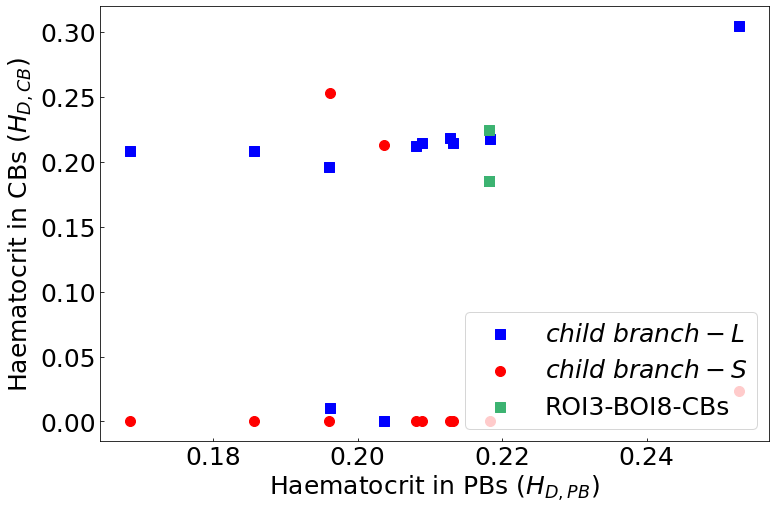
\includegraphics[width=0.6\textwidth]{images/DownstreamBifurcationHD.png}
\caption{\textit{Large haematocrit difference between the "L" and "S" child branches in each downstream bifurcation. The "L"/"S" indicate the relatively larger (blue squares) and smaller (red circles) child branches in each diverging bifurcation respectively. The green squares indicate the anomaly among all of the identified successive bifurcations.} \label{DownstreamBifurcationHD}}
\end{figure}

\noindent It was found that due to the primary assumption of axisymmetric RBC distribution in the parent branch for the empirical formulation of PSM\cite{A.R.Pries2005Mbvi, PriesAR1990BFiM}, inaccuracies will emerge when applying PSM to successive bifurcations instead of individual bifurcations across the networks. This has been demonstrated by first identifying the successive bifurcations found from simulation data (see Table \ref{SuccessiveBOIs} for the complete list) and afterwards observing the change in RBC concentration (i.e. haematocrit) in the downstream bifurcations. From Figure \ref{DownstreamBifurcationHD}, the majority of the downstream bifurcations were found to have a significantly large haematocrit difference between the child branches regardless of high or low haematocrit in the parent branches. Only one successive bifurcation (ROI3: BOI-7 $\Rightarrow$ BOI-8) indicated in green had a small haematocrit difference between the child branches of the downstream bifurcation. This features the emerging heterogeneity of RBC partitioning in successive bifurcations as the simulated RBC fluxes substantially deviate from PSM's empirical predictions. An explanation for this phenomenon was suggested by a recent study\cite{Zhou2021EmergentBifurcations} where the excessive heterogeneity is attributed to the lack of symmetrical cell-free layer (CFL) recovery in the inter-bifurcation branches. Therefore, the upstream deviations in the CFL can naturally lead to child branches deprived of RBCs even for equal blood flow split. 

% \begin{figure}[H]
% \centering
% \begin{subfigure}{0.48 \textwidth}
%     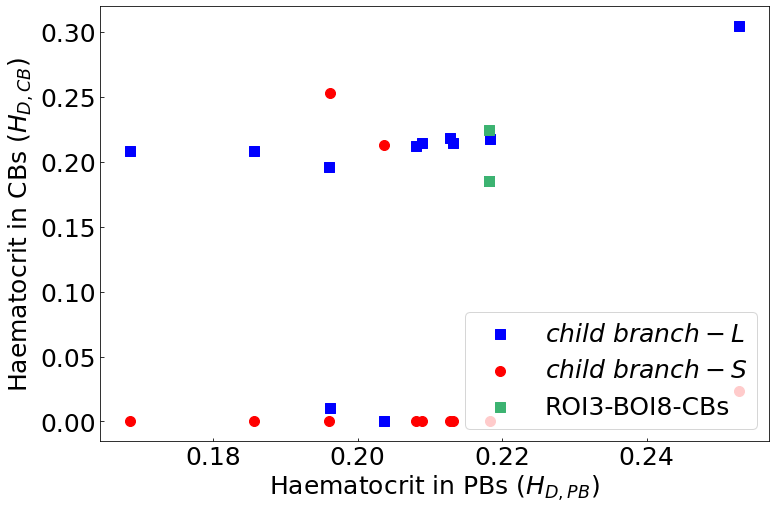
\includegraphics[width=1\textwidth]{images/DownstreamBifurcationHD.png}
%     \caption{\textit{Large haematocrit difference between the child branches of downstream bifurcations} \label{DownstreamBifurcationHD}}
% \end{subfigure}
% \hfill
% \begin{subfigure}{0.48 \textwidth}
%     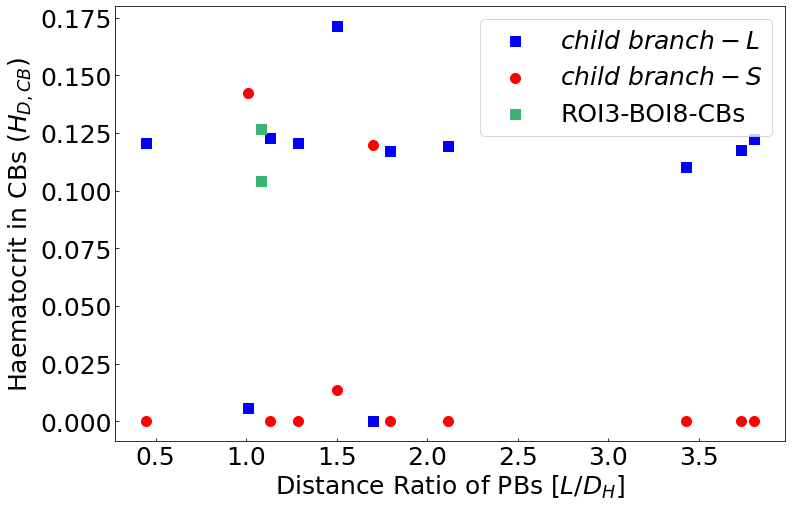
\includegraphics[width=1\textwidth]{images/DownstreamBifurcationDL.png}
%     \caption{\textit{Evaluated Hydrodynamic Diameters} \label{DownstreamBifurcationDL}}
% \end{subfigure}
% \caption{\textit{} \label{DownstreamBifurcations}}
% \end{figure}

\subsection{Breakdown in Pries Viscosity Models (\textit{in vitro} \& \textit{in vivo}) with simulation data}
\label{BreakdownInPriesViscosityModels}
\noindent Apart from examining the distributions of blood flow and haematocrit in microvascular networks, it is also important to understand the effects of blood flow properties on the flow resistance of each microvessel within the microvascular networks. To describe the behaviours of non-Newtonian blood flow in the networks of microvessels, apparent viscosity ($\mu_{app}$) is commonly used given the fact that non-continuum effects are dominant at the micro-scale. For this reason, Pries Viscosity Models\cite{Pries1992BloodHematocrit, PriesAR1994RtBF} (Equations \ref{viscosity_equation4}$-$\ref{viscosity_equation2}) were used calculated the empirical predictions to compare with the evaluated $\mu_{app}$ from simulation data (via Poiseuille's Law). On top of this, a comparison of $\mu_{app}$ calculations based on D$_{G}$ and D$_{H}$ was conducted to evaluate which diameter was the preferable input parameter for $\mu_{app}$ estimation. Also, it should be pointed out that Poiseuille’s law was primarily used to work out the apparent viscosity of blood as if it is a constant variable. However, this is actually not true in view of the fact that blood viscosity varies against shear rates and this is known as the shear-thinning effect.\cite{YELESWARAPU1998257, yeleswarapu1998evaluation, BodnarT2011Sott}


\begin{figure}[H]
\centering
\begin{subfigure}{0.48 \textwidth}
    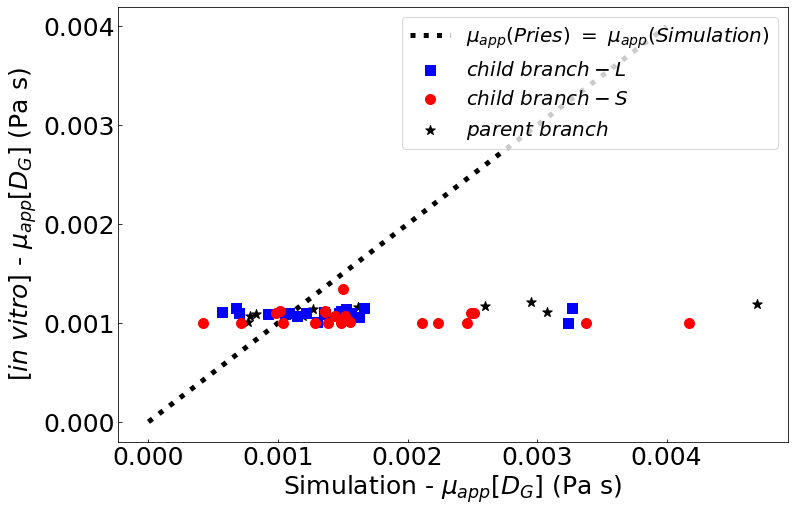
\includegraphics[width=1\textwidth]{images/InVitroApparentViscosityDG.png}
    \caption{\textit{} \label{InVitroApparentViscosityDG}}
\end{subfigure}
\hfill
\begin{subfigure}{0.48 \textwidth}
    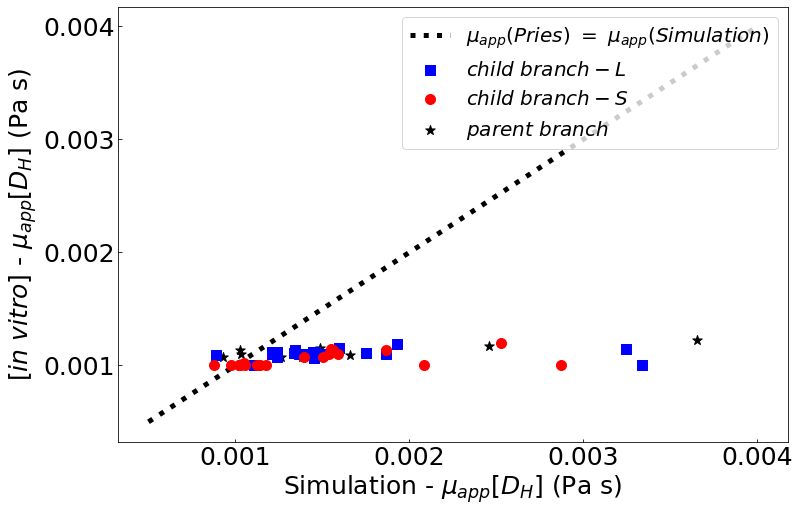
\includegraphics[width=1\textwidth]{images/InVitroApparentViscosityDH.png}
    \caption{\textit{} \label{InVitroApparentViscosityDH}}
\end{subfigure}
\begin{subfigure}{0.48 \textwidth}
    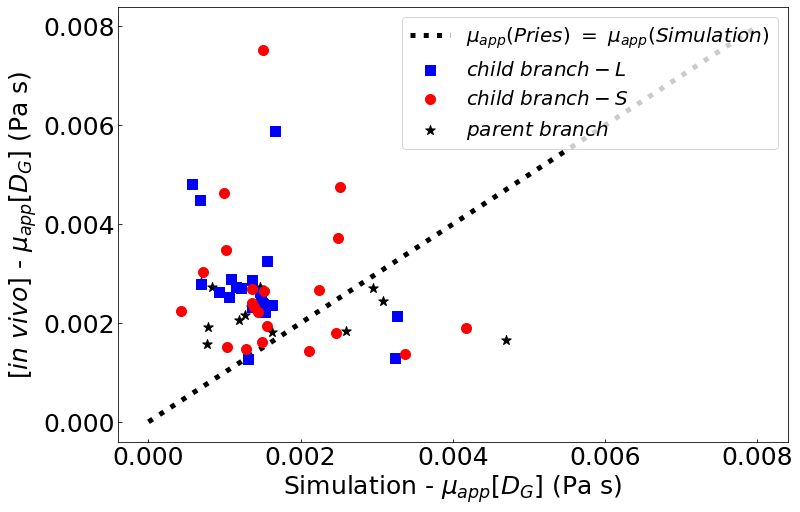
\includegraphics[width=1\textwidth]{images/InVivoApparentViscosityDG.png}
    \caption{\textit{} \label{InVivoApparentViscosityDG}}
\end{subfigure}
\hfill
\begin{subfigure}{0.48 \textwidth}
    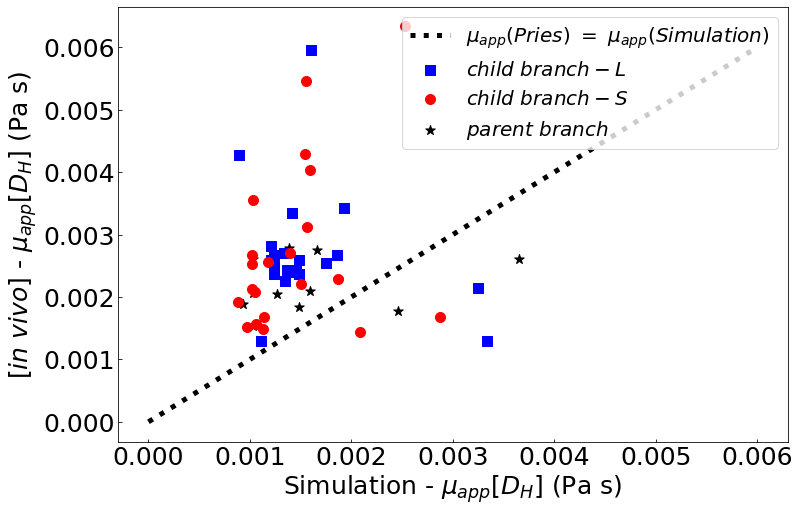
\includegraphics[width=1\textwidth]{images/InVivoApparentViscosityDH.png}
    \caption{\textit{} \label{InVivoApparentViscosityDH}}
\end{subfigure}
\caption{\textit{Comparison of simulation data against empirical predictions from Pries Viscosity Models based on both D$_{G}$ and D$_{H}$. (a$-$b) are for \textit{in vitro} and (c$-$d) for \textit{in vivo}. The "L"/"S" indicate the relatively larger (blue squares) and smaller (red circles) child branches in each diverging bifurcation respectively. The black dotted line represents when the empirical predictions and simulation data are equivalent.} \label{PriesViscosityModels}}
\end{figure}


\noindent Considering the simulation data as our reference data to test the Pries Viscosity Models, the majority of the empirical predictions from \textit{in vitro} formulation were found to be smaller than simulation data for both D$_{G}$ and D$_{H}$. This indicates that the empirical predictions from \textit{in vitro} formulation are underestimating the simulation data (Figure \ref{PriesViscosityModels}a$-$b). The primary reason for this observation is due to the irregular inner vessels that contour across the studied microvascular networks while the \textit{in vitro} empirical model was derived using long and straight glass capillary tubes. Unlike the \textit{in vitro} formulation, majority of the empirical predictions from \textit{in vivo} formulation are overestimating the simulation data (Figure \ref{PriesViscosityModels}c$-$d). This was expected because the simulation data does not consider the presence of endothelial surface layer and the nano-structured glycocalyx in contrast to the \textit{in vivo} formulation of Pries Viscosity Model.\cite{PriesAR1994RtBF} Evidence in support of this was shown in previous studies\cite{LIPOWSKY1977345, LIPOWSKY1980297, SECOMB2013470, PriesAR1994RtBF} where $\mu_{app}$ values were indeed substantially higher in microvessels than in corresponding glass tubes due to the presence of endothelial surface layer. 


\begin{table}[H]
\centering
\caption{\textit{Overall average errors of empirical prediction by Pries Viscosity Models (\textit{in vivo} \& \textit{in vitro}) in comparison to simulation data. The coloured numbers (red and green) indicate the relatively larger and smaller deviations respectively.}
\label{AdoptionOfDHoverDG}}
\scalebox{1}{
\begin{tabular}{*{5}{c}}
\dtoprule
\multirow{2}{*}{\textbf{Average Error $\%$}} & \multicolumn{2}{c}{\textbf{Pries (\textit{in vivo})}} & \multicolumn{2}{c}{\textbf{Pries (\textit{in vitro})}} \\
\cmidrule(lr){2-3} \cmidrule(lr){4-5}
& D$_{G}$ & D$_{H}$ & D$_{G}$ & D$_{H}$ \\
\midrule[0.5pt]
Larger CBs & \textcolor{red}{56.75} & \textcolor{mygreen}{51.66} & \textcolor{red}{45.45} & \textcolor{mygreen}{44.8} \\
Smaller CBs & \textcolor{red}{53.08} & \textcolor{mygreen}{49.9} & \textcolor{red}{76.2} & \textcolor{mygreen}{36.95} \\
PBs & \textcolor{red}{52.98} & \textcolor{mygreen}{41.6} & \textcolor{red}{58.4} & \textcolor{mygreen}{45.4} \\
\dbottomrule
\end{tabular}}
\end{table}

\noindent Based on the above findings, it implies that the simulation data appears to be in-between the predictions from these two empirical models and D$_{H}$ was found to be outperforming D$_{G}$ since both empirical models (\textit{in vivo} \& \textit{in vitro}) gave closer predictions. (see Table \ref{AdoptionOfDHoverDG} for complete error evaluation) Furthermore, the largest average error between the \textit{in vivo} formulation and simulation data for D$_{H}$ was found to be the larger child branches. Therefore, this points out that Pries Viscosity Model (\textit{in vivo}) becomes invalid for smaller child branches at bifurcations. 


\begin{figure}[H]
\centering
\begin{subfigure}{0.48 \textwidth}
    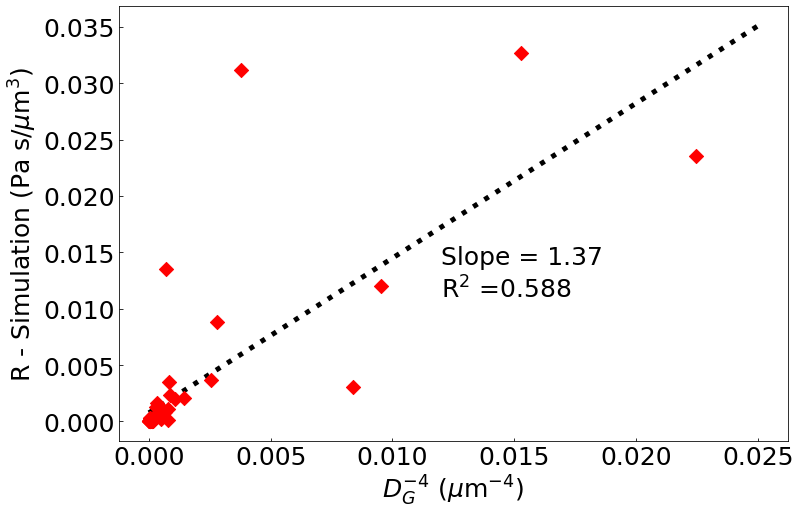
\includegraphics[width=1\textwidth]{images/PoiseuilleR_DG.png}
    \caption{\textit{} \label{PoiseuilleR_DG}}
\end{subfigure}
\hfill
\begin{subfigure}{0.48 \textwidth}
    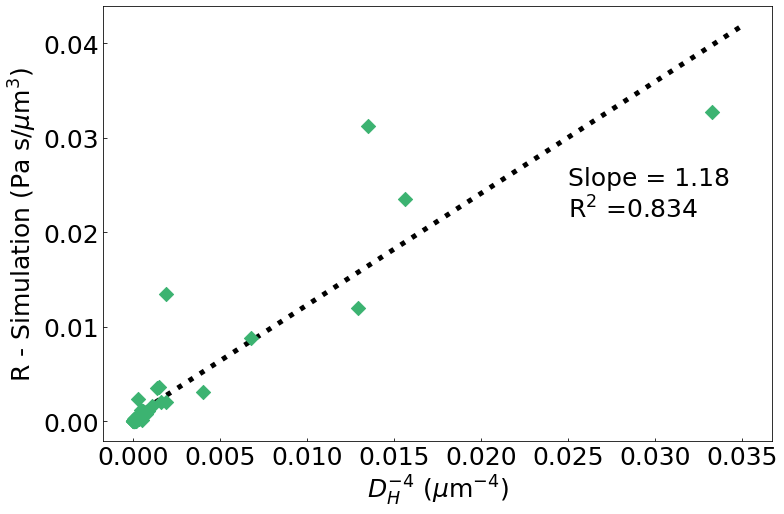
\includegraphics[width=1\textwidth]{images/PoiseuilleR_DH.png}
    \caption{\textit{} \label{PoiseuilleR_DH}}
\end{subfigure}
\caption{\textit{Correlation between flow resistance and branch diameters (D$_{G}$ \& D$_{H}$) from simulation data, including gradient and R-square values of best-fit linear lines.} \label{PoiseuilleRDs}}
\end{figure}

\noindent To further valid the adoption of D$_{H}$ over D$_{G}$, the evaluated flow resistance from simulation data was plotted as a function of D$^{-4}$ to observe how the use of D$_{H}$ in replace of D$_{G}$ contributes to a better approximation of the simulation data with Poiseuille's law. A best-fitted line was included for both diameters to obtain the R-squared value (R$^{2}$) of the fitting line as this value reflects how well the linear line captures the data distribution. From Figure \ref{PoiseuilleRDs}, the evaluated R$^{2}$ values for both D$_{G}$ and D$_{H}$ are 0.588 and 0.834 respectively. These values indicate that only 58.8\% of the residual variance of flow resistance from simulation can be explained by Poiseuille's law for D$_{G}$ whereas it is 83.4\% for D$_{H}$. Therefore, this does suggest that D$_{H}$ is indeed the preferred input parameter for $\mu_{app}$ estimation compared to D$_{G}$. As a result, the following $\mu_{app}$ estimations mentioned below will all be premised on D$_{H}$. 

\subsection{Presence of F{\aa}hr{\ae}us-Lindqvist Effect}
\label{Fahraeus_Lindqvist_Effect}
\noindent With reference to previous studies\cite{Fahrus1931THETUBES, Pries1992BloodHematocrit, SECOMB2013470} conducted, a consistent finding was observed that $\mu_{app}$ decreases substantially with decreasing tube diameters below around 300 $\mu$m and this well-known phenomenon is called the F{\aa}hr{\ae}us-Lindqvist effect. To observe whether the F{\aa}hr{\ae}us-Lindqvist effect exists in the micro-vascular networks from simulation data, graphs of relative apparent viscosity ($\mu_{rel}$) against haematocrit (H$_{D}$) and branch diameter (D$_{H}$) were plotted. From Figure \ref{Fahraeus-LindqvistEffectH}, if all the zero-haematocrit data points were excluded, there were 3 observations identified:

\begin{enumerate}
    \item Taking a horizontal viewpoint of the graph and disregarding the classification of PB, CB-L and CB-S, the overall $\mu_{rel}$ increases against $H_{D}$ except for one single outlier. 
    \item Based on a vertical viewpoint of the graph, a wide range of $\mu_{rel}$ is observed for a given $H_{D}$. This is related to the F{\aa}hr{\ae}us-Lindqvist effect which describes the non-monotonic variation of the relative apparent viscosity against vessel diameter at a fixed H$_{D}$.
    \item The data points of CB-L and CB-S are more or less overlapped while majority of the PB data points are at the bottom of the graph which indicates having relatively smaller $\mu_{rel}$. 
\end{enumerate}

\begin{figure}[H]
\centering
\begin{subfigure}{0.50 \textwidth}
    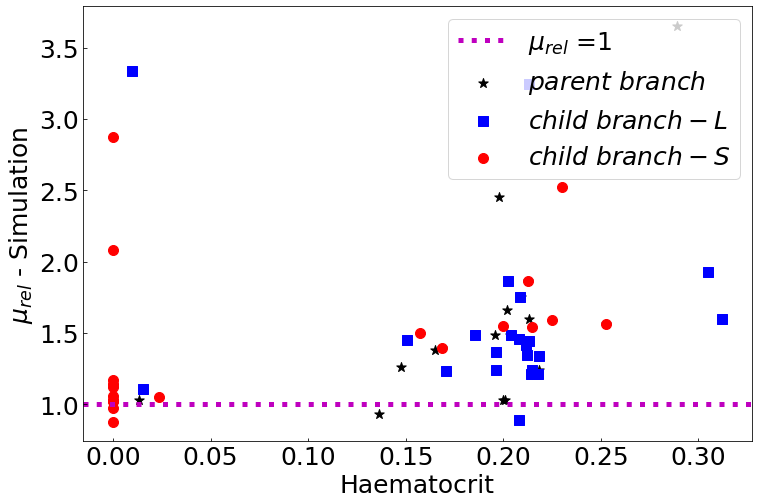
\includegraphics[width=1\textwidth]{images/Fahraeus-LindqvistEffectH.png}
    \caption{\textit{Graph of $\mu_{rel}$ against H$_{D}$ with classification of PB, CB-L and CB-S.} \label{Fahraeus-LindqvistEffectH}}
\end{subfigure}
\hfill
\begin{subfigure}{0.48 \textwidth}
    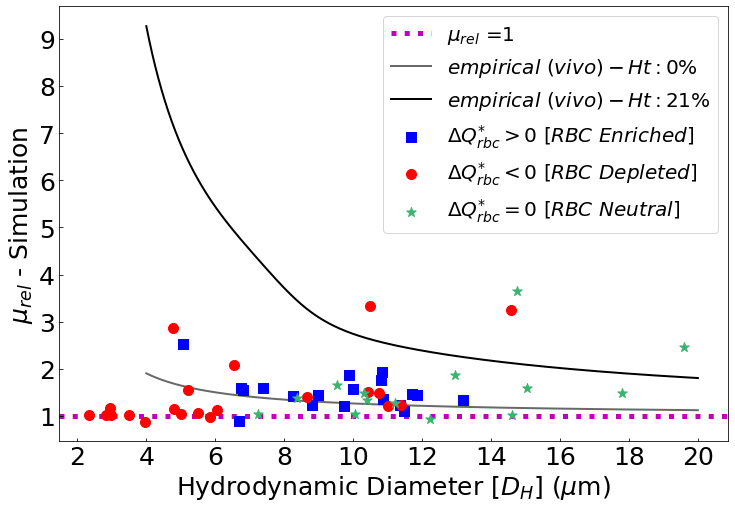
\includegraphics[width=1\textwidth]{images/Fahraeus-LindqvistEffectD.png}
    \caption{\textit{Graph of $\mu_{rel}$ against D$_{H}$ with classification of neutral, RBC-enriched and RBC-depleted branches} \label{Fahraeus-LindqvistEffectD}}
\end{subfigure}
\caption{\textit{Demonstration of the presence of F{\aa}hr{\ae}us-Lindqvist effect within micro-vascular networks from simulation data. The purple dotted line represents the ratio of apparent blood viscosity against plasma viscosity is equivalent to 1.} \label{Fahraeus-LindqvistEffects}}
\end{figure}

\noindent For Figure \ref{Fahraeus-LindqvistEffectD}, two empirical lines with a fixed H$_{D}$ of 0\% and 21\% were included to observe how much the simulation data deviates from empirical prediction. These two values were selected because the majority of the RBC-depleted and RBC-enriched branches were found around either the 0\% or 21\% haematocrit levels as shown in Figure \ref{DisproportionalityIndexHD}. However, we do have to take note that this may not be an accurate evaluation as some branches do not have an exact haematocrit of either 0\% or 21\%. In Figure \ref{Fahraeus-LindqvistEffectD}, it was observed that the majority of the simulation data do significantly deviate from empirical predictions and a vast majority of the RBC-depleted branches have a lower apparent blood viscosity than the RBC-enriched branches. Furthermore, branch diameters smaller than 8$\mu$m (diameter of a freely suspended human RBC) tend to have a greater deviation between simulation data and empirical predictions compared to branch diameters larger than 8$\mu$m. \\

\noindent According to these observations mentioned above, it implies that the simulation data was unable to clearly demonstrate the presence of F{\aa}hr{\ae}us-Lindqvist effect. The primary reason could be the difference in branch length ($L$) within the micro-vascular networks from simulation data compared to previous experimental studies. 

% Importance of Branch Length in Apparent Viscosity Estimation
\subsection{Importance of Branch Length and Distance Ratio}
\label{BranchLength_DistanceRatio}
\noindent Based on the deviations of simulation viscosity from empirical predictions, the potential source of the deviation could be due to the branch length. Hence, we now focus our attention on the importance of branch length for $\mu_{app}$ estimations. However, instead of directly characterising $\mu_{rel}$ against the measure of the absolute branch length ($L$), another parameter called distance ratio (ratio of branch length to branch diameter) was considered with a classification of "in vivo favoured" and "in vitro favoured" branches. The evaluated deviations between simulation data against \textit{in vivo} and \textit{in vitro} empirical predictions are represented as vivo-ERR and vitro-ERR respectively. 

\begin{figure}[H]
\centering
\begin{subfigure}{0.45 \textwidth}
    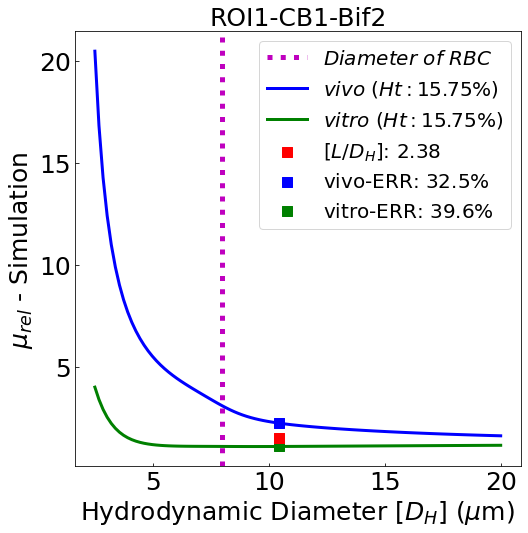
\includegraphics[width=0.92\textwidth]{images/DeviationsViscosity1.png}
    \caption{\textit{} \label{DeviationsViscosity1}}
\end{subfigure}
\hfill
\begin{subfigure}{0.45 \textwidth}
    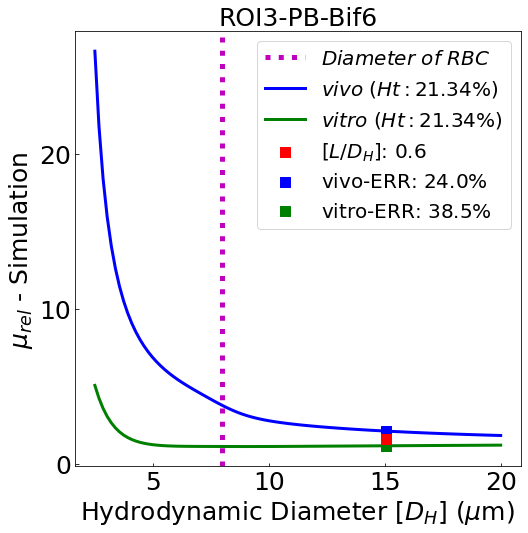
\includegraphics[width=0.92\textwidth]{images/DeviationsViscosity2.png}
    \caption{\textit{} \label{DeviationsViscosity2}}
\end{subfigure}
\hfill
\begin{subfigure}{0.45 \textwidth}
    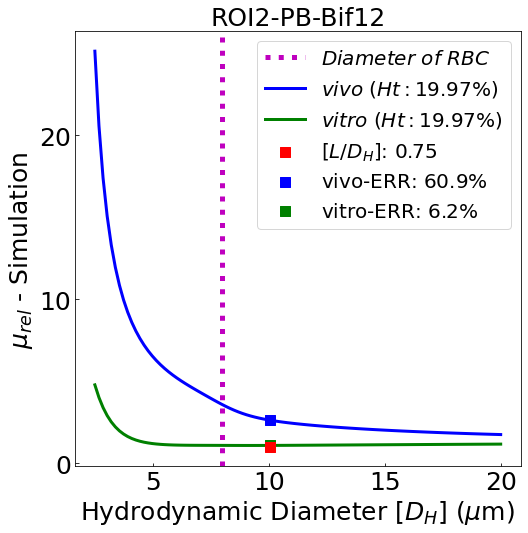
\includegraphics[width=0.92\textwidth]{images/DeviationsViscosity3.png}
    \caption{\textit{} \label{DeviationsViscosity3}}
\end{subfigure}
\hfill
\begin{subfigure}{0.45 \textwidth}
    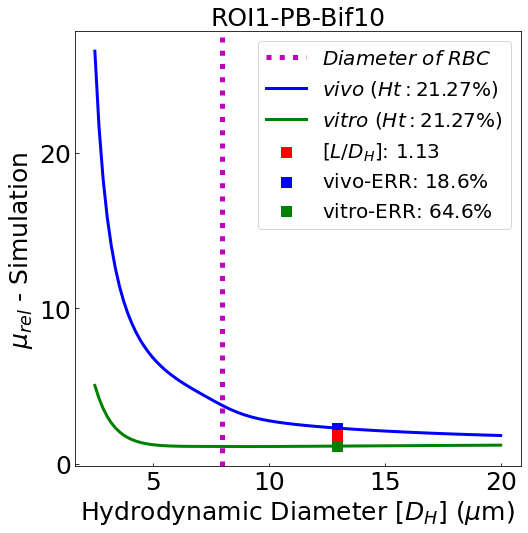
\includegraphics[width=0.92\textwidth]{images/DeviationsViscosity4.png}
    \caption{\textit{} \label{DeviationsViscosity4}}
\end{subfigure}
\caption{\textit{Comparison of simulation data (red) against empirical predictions of both Pries Viscosity Models (blue and green) within studied networks. The solid lines represent the empirical models and the purple dotted line indicates the average RBC diameter. (a$-$b) Exemplar individual branches with simulation data in-between empirical predictions. (c$-$d) Examples of "in vitro favoured" and "in vivo favoured" branches respectively.} \label{DeviationsVisocity}}
\end{figure}

\noindent Kindly note that the context of "in vivo favoured" and "in vitro favoured" is a relative notion between the vivo-ERR and vitro-ERR in each branch. This means if vivo-ERR $>$ vitro-ERR in a given branch, that branch is "in vitro favoured" (whereas the branch is "in vivo favoured" if vivo-ERR $<$ vitro-ERR). Based on this assessment, we hypothesized that the smaller distance ratio ($L$/D$_{H}$) branches should match relatively better with \textit{in vivo} formulation instead of \textit{in vitro} formulation. \\

\noindent In addition to this, it was previously mentioned in Section \ref{Fahraeus_Lindqvist_Effect} that the $\mu_{app}$ values evaluated from simulation data appear to be in-between the empirical predictions from both Pries Viscosity Models (\textit{in vitro} and \textit{in vivo}). To justify this claim, simulation data with non-zero haematocrit in each individual branch were compared to the empirical predictions from both \textit{in vitro} and \textit{in vivo} formulations. The results for the individual branches in ROI1, ROI2 and ROI3 are listed in Appendix \ref{EvaluationOfSimulationDataVSPVM} (see Figures \ref{DeviationsViscosity-ROI1}$-$\ref{DeviationsViscosity-ROI3}). The results indicated 29 branches out of 57 were classified as "in vitro favoured" while the remaining 28 branches were "in vivo favoured". An illustration of 4 individual branches is presented (see Figure \ref{DeviationsVisocity}) for which the first 2 examples indicate the actual apparent viscosity was somewhere between both Pries Viscosity Models while the last 2 examples show the classification of "\textit{in vitro} favoured" and "\textit{in vivo} favoured" branches. 


\begin{figure}[H]
\centering
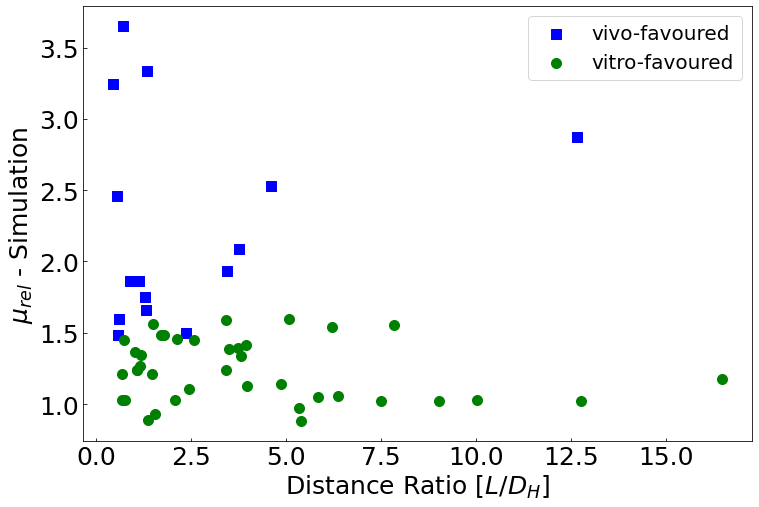
\includegraphics[width=0.75\textwidth]{images/RelativeApparentViscosityVSDistanceRatio.png}
\caption{\textit{Correlation between relative apparent blood viscosity against distance ratio} \label{RelativeApparentViscosityVSDistanceRatio}}
\end{figure}

\noindent From Figure \ref{RelativeApparentViscosityVSDistanceRatio}, it was observed that majority of the "\textit{in vivo} favoured" branches have a variation of $\mu_{rel}$ (ranging from 1.3 up to 3.6) for a given distance ratio. Whereas for "\textit{in vitro} favoured" branches, it was noticed to have a relatively constant $\mu_{rel}$ (limited up to around 1.5) across the entire range of distance ratios. It was also apparent that the range of distance ratio for "\textit{in vivo} favoured" branches excluding one single outlier was found within 0 to 5 while it was across the whole range for "\textit{in vitro} favoured" branches. These findings concur with the initial hypothesis whereby the smaller $L$/D$_{H}$ branches are usually better matched with the \textit{in vivo} formulation of Pries Viscosity Model where "\textit{in vivo} favoured" branches lie within a distinct range unlike "\textit{in vitro} favoured" branches. Therefore, this highlights the importance of considering the branch length for $\mu_{app}$ estimation because the majority of the branches from simulation data are relatively shorter compared to the extended glass tubes for the \textit{in vitro} model and the long vessels for the \textit{in vivo} model. \\


\noindent Another apparent observation found in Figure \ref{RelativeApparentViscosityVSDistanceRatio} was the inverse relationship between $\mu_{rel}$ and distance ratio which also implies that short branches tend to have a higher relative apparent blood viscosity. A similar way of describing this is that the apparent blood viscosity ($\mu_{app}$) in any branch will increase when the branch length ($L$) decreases. This is an interesting result observed as it is not something that can be observed from Hagen-Poiseuile's equation (correlation between $\mu_{app}$ and $L$). Also, under Poiseuille's law, a fully developed flow is assumed as the effects of the conditions at the entrance of each branch were neglected. Therefore, a plausible reason behind this observation could be due to the entrance effect where it requires more energy for the RBCs to move into the branch, but once the RBCs are inside the branch, it seems easier for the RBCs to continue flowing. This shows that a closer look at the correlation between $L$ and D$_{H}$ will be required to disentangle their contributions on the $\mu_{app}$ which influences the asymmetric RBC distribution across micro-vascular networks. \\

\noindent In addition to this, the dependence of $\lvert Q^{*}_{rbc} - Q^{*}_{blood} \rvert$ on the distance ratio was also considered (see Figure \ref{DisproportionalityIndexDistanceRatio}). Following the practice of Balogh and Bagchi\cite{Balogh2018}, the quantity of $\lvert Q^{*}_{rbc} - Q^{*}_{blood} \rvert$ was considered as a measure of disproportionality in RBC partitioning. With reference to this, it was observed that the $\lvert Q^{*}_{rbc} - Q^{*}_{blood} \rvert$ value increases with decreasing distance ratio. Furthermore, we have noticed that across the studied networks, shorter branches tend to have a relatively larger diameter (and vice versa) within a given bifurcation. This suggests that on average the RBC partitioning tend to become less disproportionate as the branch length increases. However, this might not be true given that $L$/D$_{H}$ will always have a tendency to become smaller with increasing D$_{H}$, unless the length of a branch grows more strongly than D$_{H}$. Therefore, understanding the correlation between $L$ and D$_{H}$ will help justify the influence of $L$/D$_{H}$ onto the degree of disproportionality in RBC partitioning.\\



\begin{figure}[H]
\centering
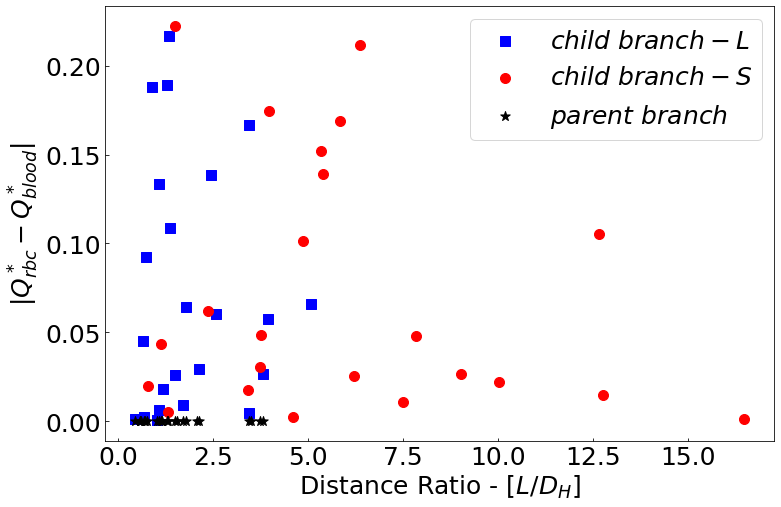
\includegraphics[width=0.75\textwidth]{images/DisproportionalityIndexDistanceRatio.png}
\caption{\textit{Influence of the distance ratio on the degree of disproportionality in RBC partitioning. The "L"/"S" indicate the relatively larger (blue squares) and smaller (red circles) child branches in each diverging bifurcation respectively.} \label{DisproportionalityIndexDistanceRatio}}
\end{figure}

\subsection{Contributing factors to Asymmetric RBC Distribution}
\label{ContributingFactorsTOAsymmetricRBCDistribution}
\noindent Having demonstrated that there is a negative correlation between $\mu_{rel}$ and $L$/D$_{H}$ in Figure \ref{RelativeApparentViscosityVSDistanceRatio}, $L$/D$_{H}$ could be an additional contributing factor on apparent viscosity apart from the known effects of  D$_{H}$ and H$_{D}$ on apparent viscosity. It is well-known that the apparent viscosity in micro-vessels are dominated by the thickness of the cell-free layer (CFL) and a certain length is required in order for the CFL to fully develop in a branch. This means the relative thickness of CFL to branch diameter increases with branch length which will affect the apparent viscosity of blood in the branch. So, the degree to which the CFL is recovered after a bifurcating point should greatly affect the apparent viscosity in the downstream branch. \\

\noindent A closer look at the distribution of $L$ against D$_{H}$ (see Figure \ref{BranchLengthVSBranchDiamete}) shows a negative correlation between $L$ and D$_{H}$ was observed where the branch length decreases with branch diameter. Given that the context of "longer" and "shorter" is a relative comparison between the two child branches in each bifurcation, the majority of the longer child branches were found to have smaller diameters while shorter branches have larger diameters. To evaluate the potential of a negative correlation, the Pearson correlation coefficient (r) was calculated to measure the ratio of the covariance of branch diameter and branch length to the product of their standard deviations. This gives us the measure of the linear relationship between these two parameters. From Figure \ref{BranchLengthVSBranchDiamete}, the value r $=$ -0.535 indicates a strong negative correlation (0.5 $<$ $\lvert$ r $\rvert$ $<$ 1) between the length and diameter of vessels within the studied networks. Furthermore, a p-value $<$ 0.001 was calculated which suggests that the results obtained were statistically highly significant and are less than 1 in 1000 chance of being wrong. Therefore, it is apparent that the negative correlation does clearly exist within the studied networks. 


\begin{figure}[H]
\centering
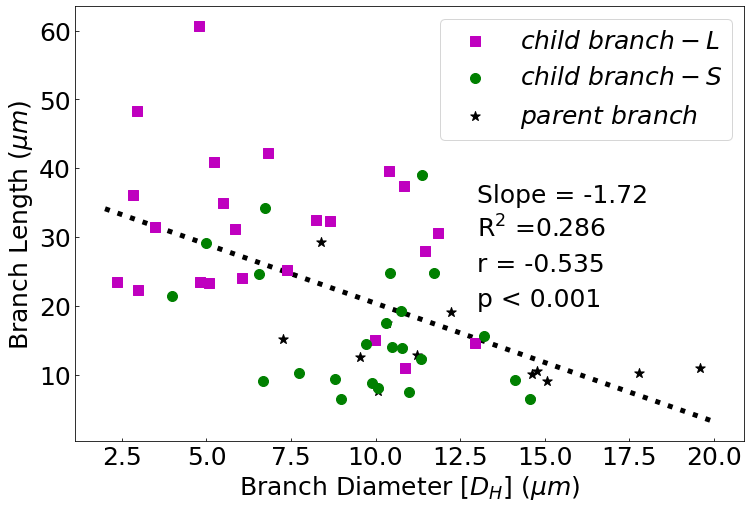
\includegraphics[width=0.8\textwidth]{images/BranchLengthVSBranchDiameter.png}
\caption{\textit{Distribution of branch length against branch diameter with best-fitted line. The "L"/"S" indicate the relatively longer (purple squares) and shorter (green circles) child branches in each diverging bifurcation respectively.} \label{BranchLengthVSBranchDiamete}}
\end{figure}

\noindent Considering that the branches from simulation data have limited branch length, most of the CFLs are not fully developed in the branches across all of the ROIs. The lack of symmetrical CFL recovery could be due to the migration of RBCs induced by boundary interactions where the RBCs tend to migrate away from the solid boundaries (i.e. vessel walls) when suspended in a shear flow. Therefore, the lack of CFL recovery and insufficient RBC migration due to limited interbifurcation distances (i.e. $L$/D$_{H}$ for the branch between bifurcations) are the causes for the deviation between simulation data and empirical predictions from Pries Viscosity Models (\textit{in-vivo} and \textit{in-vitro}). In other words, the smaller the $L$/D$_{H}$, the more underdeveloped the CFL in the downstream branch will be and hence, the cross-sectional distribution of RBCs is disturbed after the bifurcation and will require a certain distance (i.e. $L$/D$_{H}$) to recover back to its original shape of the haematocrit profile. 

\subsection{Invalid Data Points within Post-Processing Data}
\label{InvalidDataPoints}
% Include a short discussion in the section about the data points that may have additional errors due to assumptions made and the type of data analysis performed, given that the vessel network we have worked on is rather “messy” instead of ideal. 

\noindent In the process of data extraction and data analysis, several noticeable outliers and additional errors were detected and removed in order to visualise most of the data points properly. (see Tables \ref{Outliers} and \ref{CBwithoutRBCs}) Most of such data points were observed due to the difficulty of accurately measuring extremely low blood flow rates of a given branch in the studied networks. These identified branches have generally small diameters and most often do not have any RBCs present. These measurements of extremely low blood flow rates are usually inaccurate and this affects the calculations of flow resistance which subsequently affects the evaluated apparent viscosity via Poiseuille's Law. \\

\noindent Another plausible explanation for additional errors to occur would be due to the estimation of pressure drops across each branch within the studied networks. This was because the pressure drops across a given branch (i.e. outliers) obtained from plasma-only simulation data were found to be greater than that from blood flow simulation data. Therefore, this affects the calculations for flow resistance because of the issues in pressure measurements. Considering that flow resistance ratio (i.e. the fraction of blood flow resistance against plasma flow resistance) is equivalent to relative apparent viscosity, this explains why some of the data points have $\mu_{rel}$ $<$ 1 when it is supposed to be either equal or greater than 1 (see Table \ref{AdditionalErrors} for examples). 

\begin{table}[H]
\centering
\caption{\textit{List of branches with additional errors due to assumptions made}
\label{AdditionalErrors}}
\scalebox{0.95}{
\begin{tabular}{*{4}{c}}
\dtoprule
\multirow{2}{*}{\textbf{Branches}} & \multirow{2}{*}{\textbf{Flowrate (Q)}} & \multirow{2}{*}{\textbf{Pressure Drop ($\Delta$P)}} & \textbf{Flow Resistance} \\
& & & \textbf{Ratio (R$^{*}$)} \\
\midrule[0.5pt]
ROI1-BOI7-CB2 & \thead{Blood flowrate\\ $>$ plasma flowrate} & \thead{Plasma pressure drop\\ > blood pressure drop} & R$^{*}$ $<<$ 1 \\
\midrule[0.5pt]
ROI2-BOI7-CB2 & \thead{Blood flowrate\\ $>$ plasma flowrate} & \thead{Plasma pressure drop\\ > blood pressure drop} & R$^{*}$ $<<$ 1 \\
\midrule[0.5pt]
ROI2-BOI15-PB & \thead{Plasma flowrate almost\\ equivalent to blood flowrate} & \thead{Plasma pressure drop\\ > blood pressure drop} & R$^{*}$ $<$ 1 \\
\midrule[0.5pt]
ROI3-BOI9-CB1 & \thead{Plasma flowrate almost\\ equivalent to blood flowrate} & \thead{Plasma pressure drop\\ > blood pressure drop} & R$^{*}$ $<$ 1 \\
\dbottomrule
\end{tabular}}
\end{table}

\noindent Given that Poiseuille's Law was used to work out the apparent viscosity from simulation data, this assumes blood viscosity is a constant variable (i.e Newtonian fluid) which is not true due to the complex rheological behaviours associated with RBCs in micro-vessels such as the shear-thinning effect. On top of this, the microvascular networks investigated were rather "messy" instead of ideal due to the geometric irregularities of vessels in the studied networks. Therefore, some abnormalities and outliers are to be expected based on the given assumptions. Overall, the majority of the data points analysed were applicable for data analysis while the identified outliers are appropriately reasoned. \\



%----------------------------------------------------------------------------------------
%	CONCLUSION AND FUTURE WORKS SECTION
%----------------------------------------------------------------------------------------
\newpage
\section{Conclusions \& Future Works}
\noindent In summary, the findings of this study have gathered a few strong conclusions from this research project which could act as a stepping stone to formulate a simplified yet robust reduced-order model for future investigations. Firstly, hydrodynamic diameter is the preferable input parameter for apparent viscosity estimations compared to geometric diameter. Secondly, RBC distribution within studied networks is flow-mediated and the presence of plasma skimming effect was demonstrated from simulation data. Thirdly, the distance ratio ($L$/D$_{H}$) could be an additional contributing factor to relative apparent viscosity which explains the development of CFL recovery. Hence, this will influence the asymmetric RBC distribution across the network apart from the known effects of D$_{H}$ and H$_{D}$ on apparent viscosity. Last but not least, the heterogeneity of RBC distribution is attributed to the upstream perturbation in the CFL and the lack of CFL recovery between consecutive bifurcations. Therefore, with the accumulation of high-fidelity simulation data of blood flow in complex microvascular networks, a robust reduced-order model or extended constitutive models can be developed to improve the estimation of apparent viscosities. This can provide more reliable flow resistance estimations within a network while minimising the requirement for computational power. Furthermore, we will be able to gain a better understanding of the RBC distribution mechanisms at the micro-circulation level and characterise the cellular character embedded in the general blood flow. \\

\noindent Nevertheless, there are still numerous missing gaps that should be looked into for future works in order to achieve a robust reduced-order model that will not only aid future investigations but also clarify how certain effects propagate at an entire network level. Some of the considerations are:

\begin{enumerate}
    \item Consider the presence of WBCs or platelets in blood flow or the presence of endothelial surface layer on vessel walls in the networks.
    \item Consideration of other plausible mechanisms such as separation surface cross-over, lingering and jamming effects of RBCs at the bifurcation points. 
    \item Increase haematocrit in simulation to validate the importance of hydrodynamic diameter over geometric diameter in Pries's PSM and viscosity models. 
    \item Suggestions on how to quantify the blood flow entrance effect with $L$/D$_{H}$:
    \begin{itemize}
        \item Quantification of CFL thickness will be required to correlate with $L$/D$_{H}$ in order to justify the relative significance of the CFL in each vessel branch .
        \item Identify the critical threshold of $L$/D$_{H}$ with haematocrit for apparent viscosity between simulation data and empirical predictions across the networks.  
    \end{itemize}
\end{enumerate}



% \section{Emerging Challenges \& Opportunities}
% \begin{itemize}
%     \item Find out number of occurrences of the lingering/jamming effects in the 3D complex blood flow networks. 
%     \item 
% \end{itemize}




% discover new insights and phenomena in microcirculatory blood flow

% Last but not least, 
% This allows us to formulate reduced-order models that are capable of predicting and describing the haemodynamics in microcirculations. 



%----------------------------------------------------------------------------------------
%	REFERENCES SECTION
%----------------------------------------------------------------------------------------
\newpage
\bibliographystyle{IEEEtran}
\bibliography{References}
\addcontentsline{toc}{section}{References}


%----------------------------------------------------------------------------------------
%	APPENDICES SECTION
%----------------------------------------------------------------------------------------
\uselandscape
\begin{appendices}
\section{Supplementary Materials \& Analysis}
\subsection{Flow Patterns across studied microvascular networks}
\begin{figure}[H]
\centering
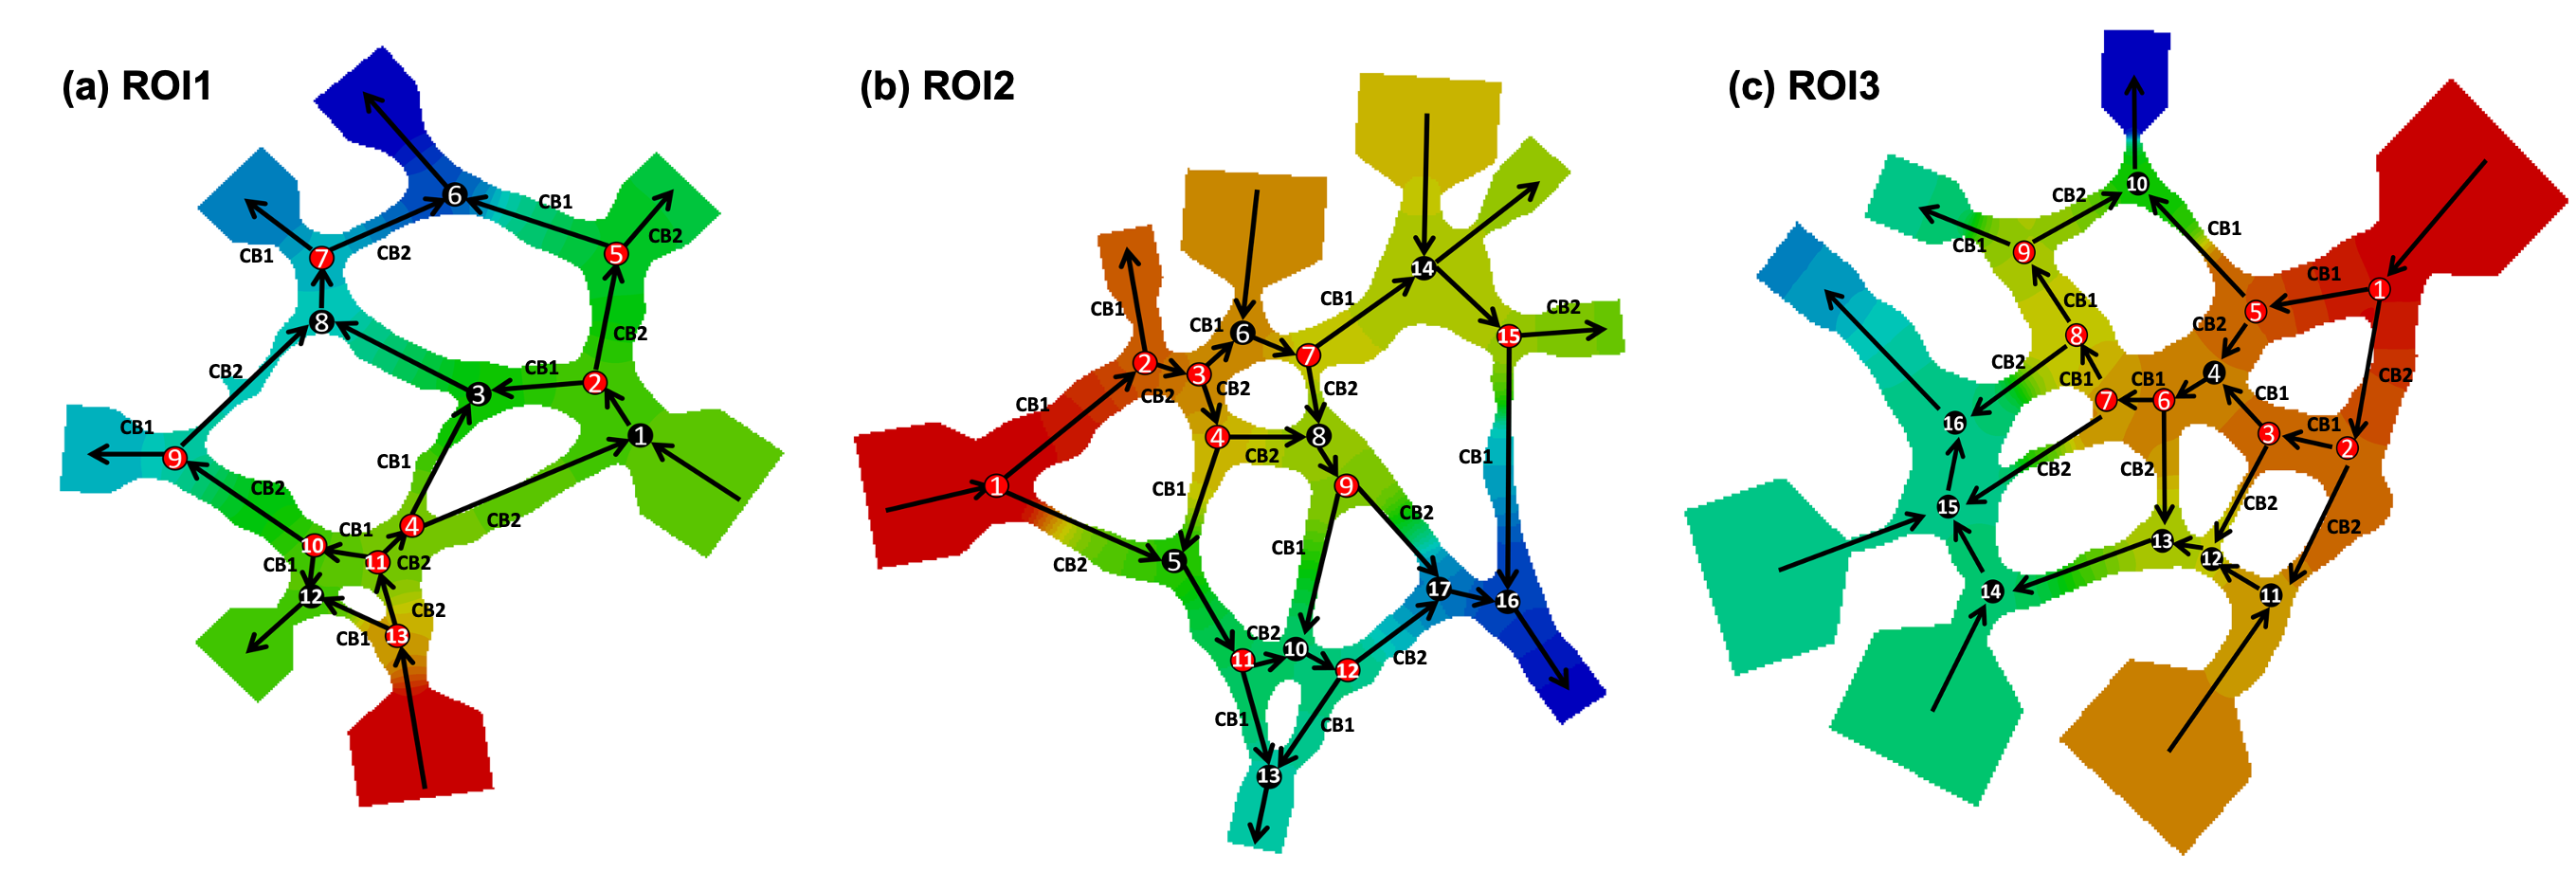
\includegraphics[width=1\textwidth]{images/ROI-Diagrams.png}
\caption{\textit{An illustration of the identified flow patterns and diverging bifurcations within ROI-1, ROI-2 and ROI-3. The diverging and converging bifurcations within each ROI are marked with red and black circles respectively. The arrows represent the direction of blood flow in each individual branch, while the background contour points out the the pressure field where a warmer colour (E.g red) represents higher pressure.} \label{ROIs}}
\end{figure}



% \begin{figure}[H]
% \centering
% \begin{subfigure}{0.33 \textwidth}
%     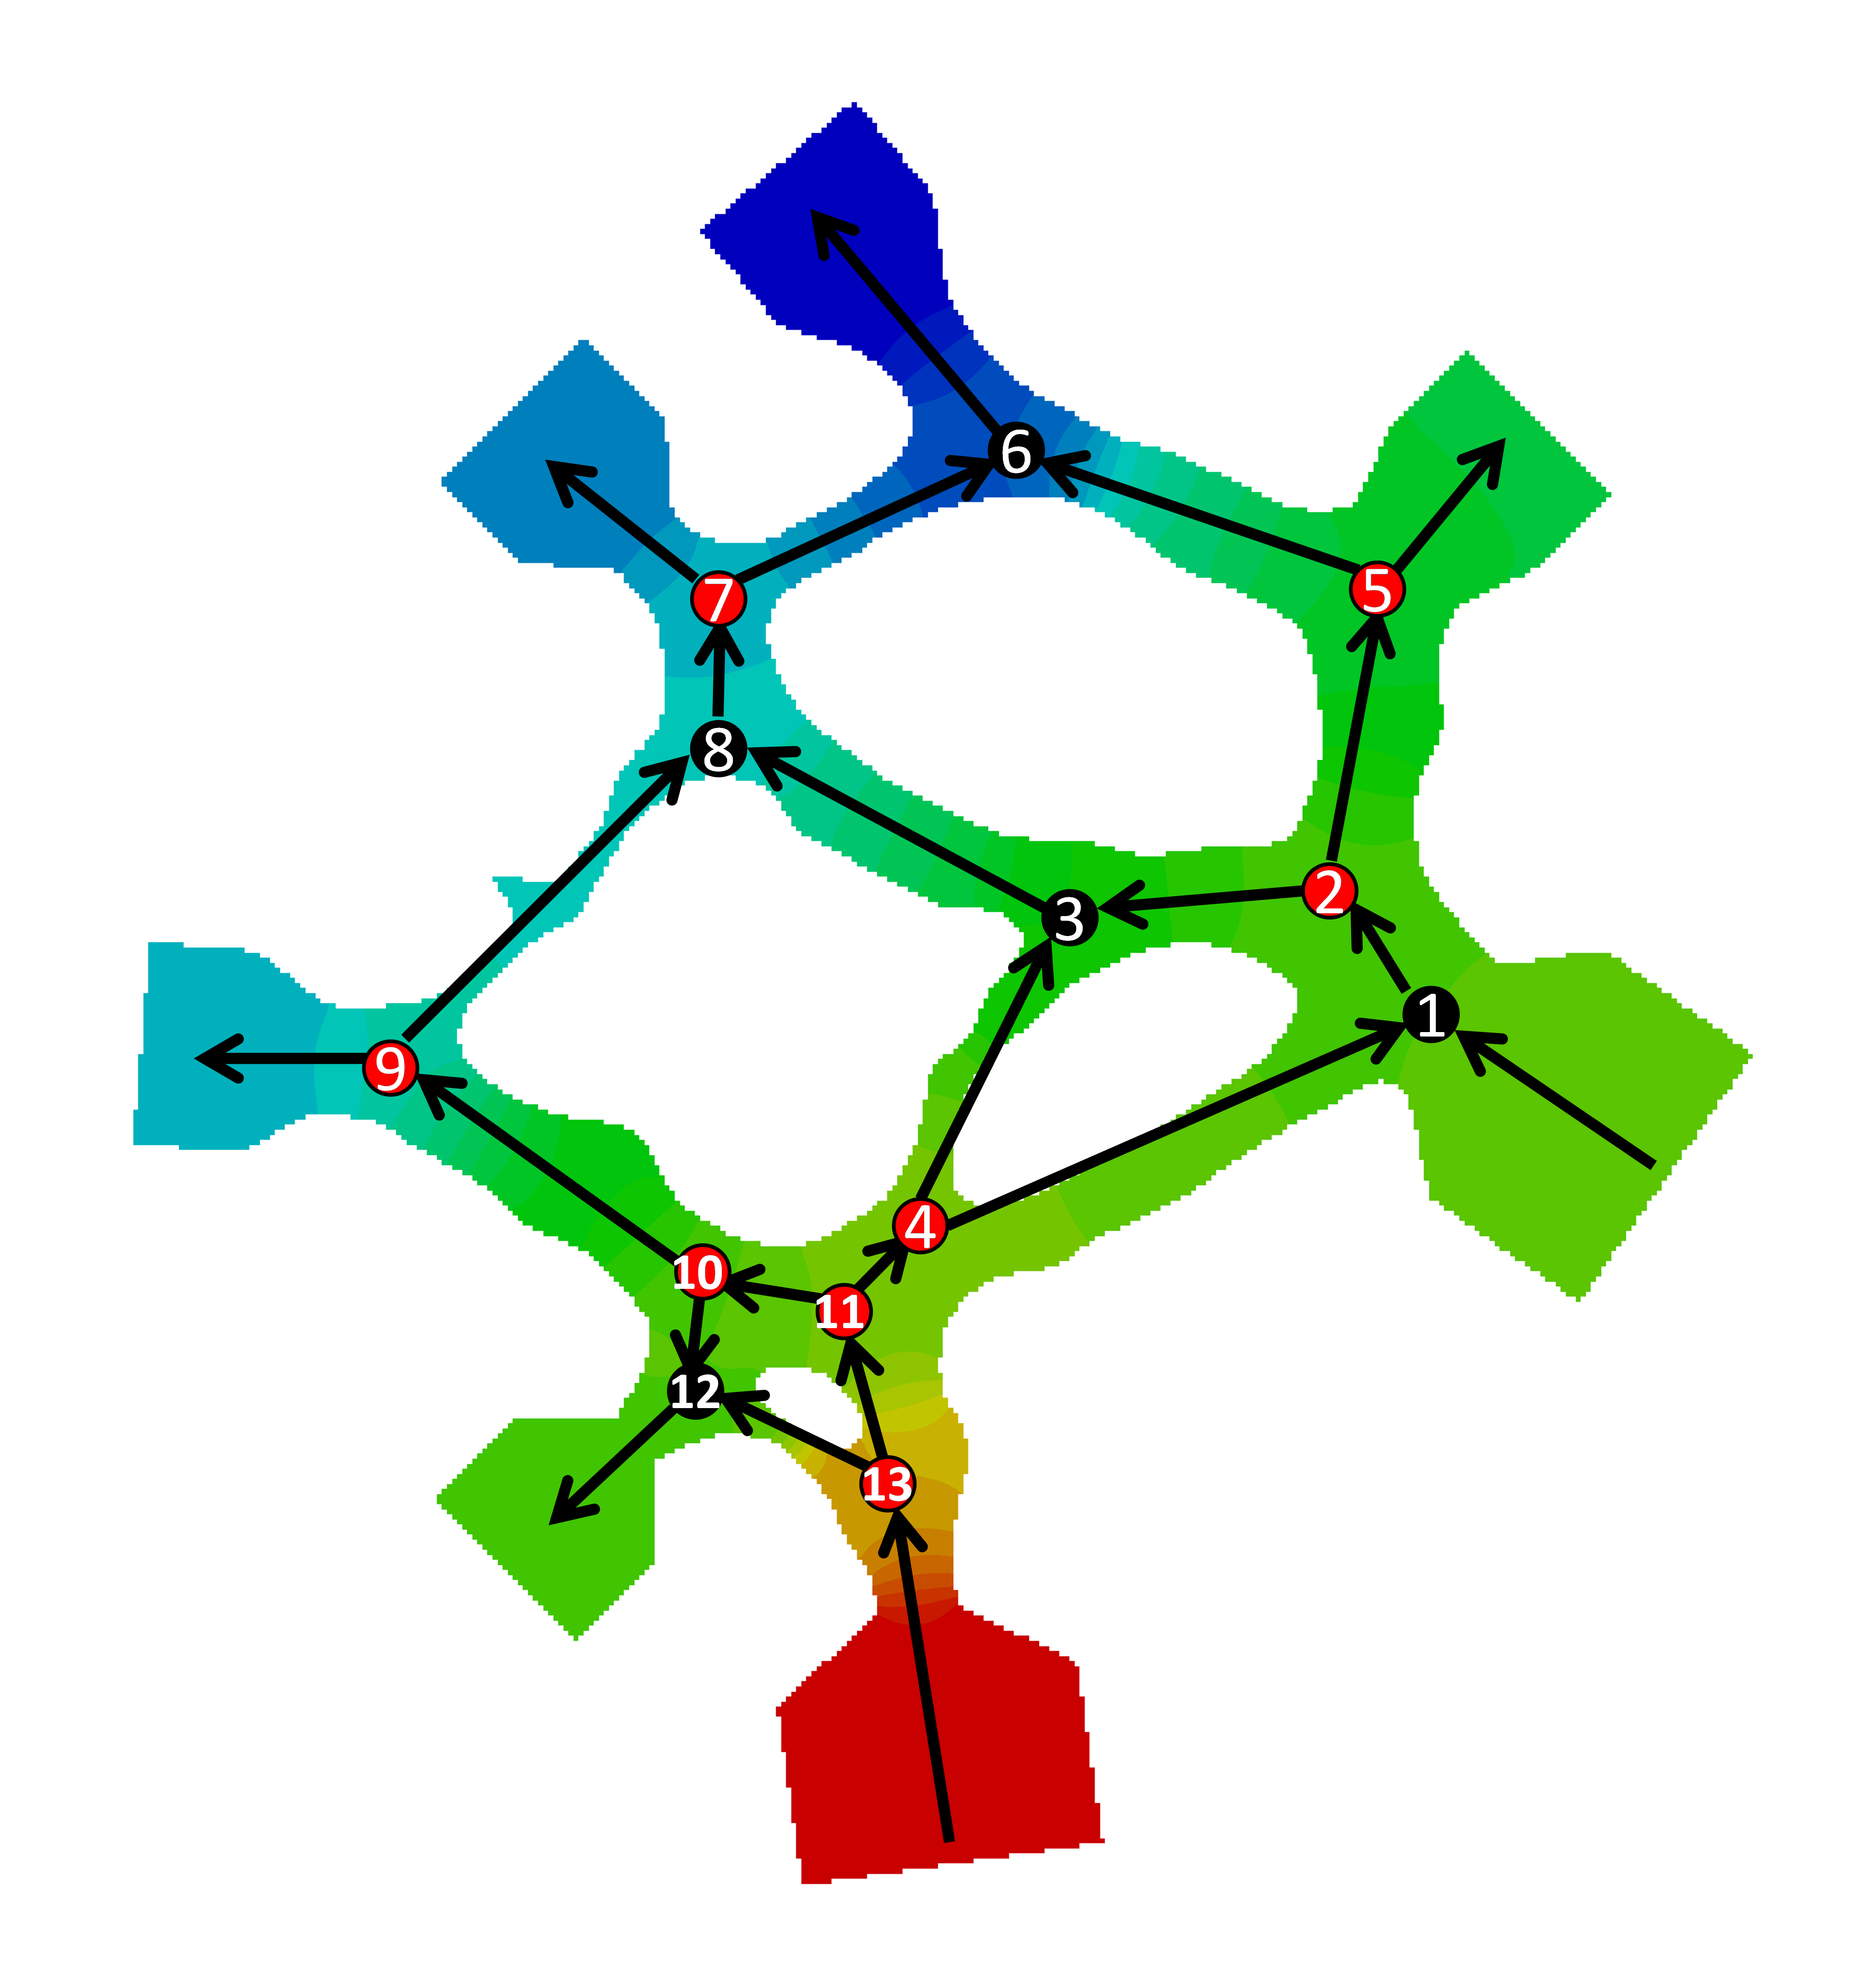
\includegraphics[width=1\textwidth]{images/bifurcations_ROI-1.png}
%     \caption{\textit{Schematic diagram of the ROI1 blood flow network which consists of 8 diverging bifurcations and 19 independent branches.} \label{ROI1}}
% \end{subfigure}
% \hfill
% \begin{subfigure}{0.33 \textwidth}
%     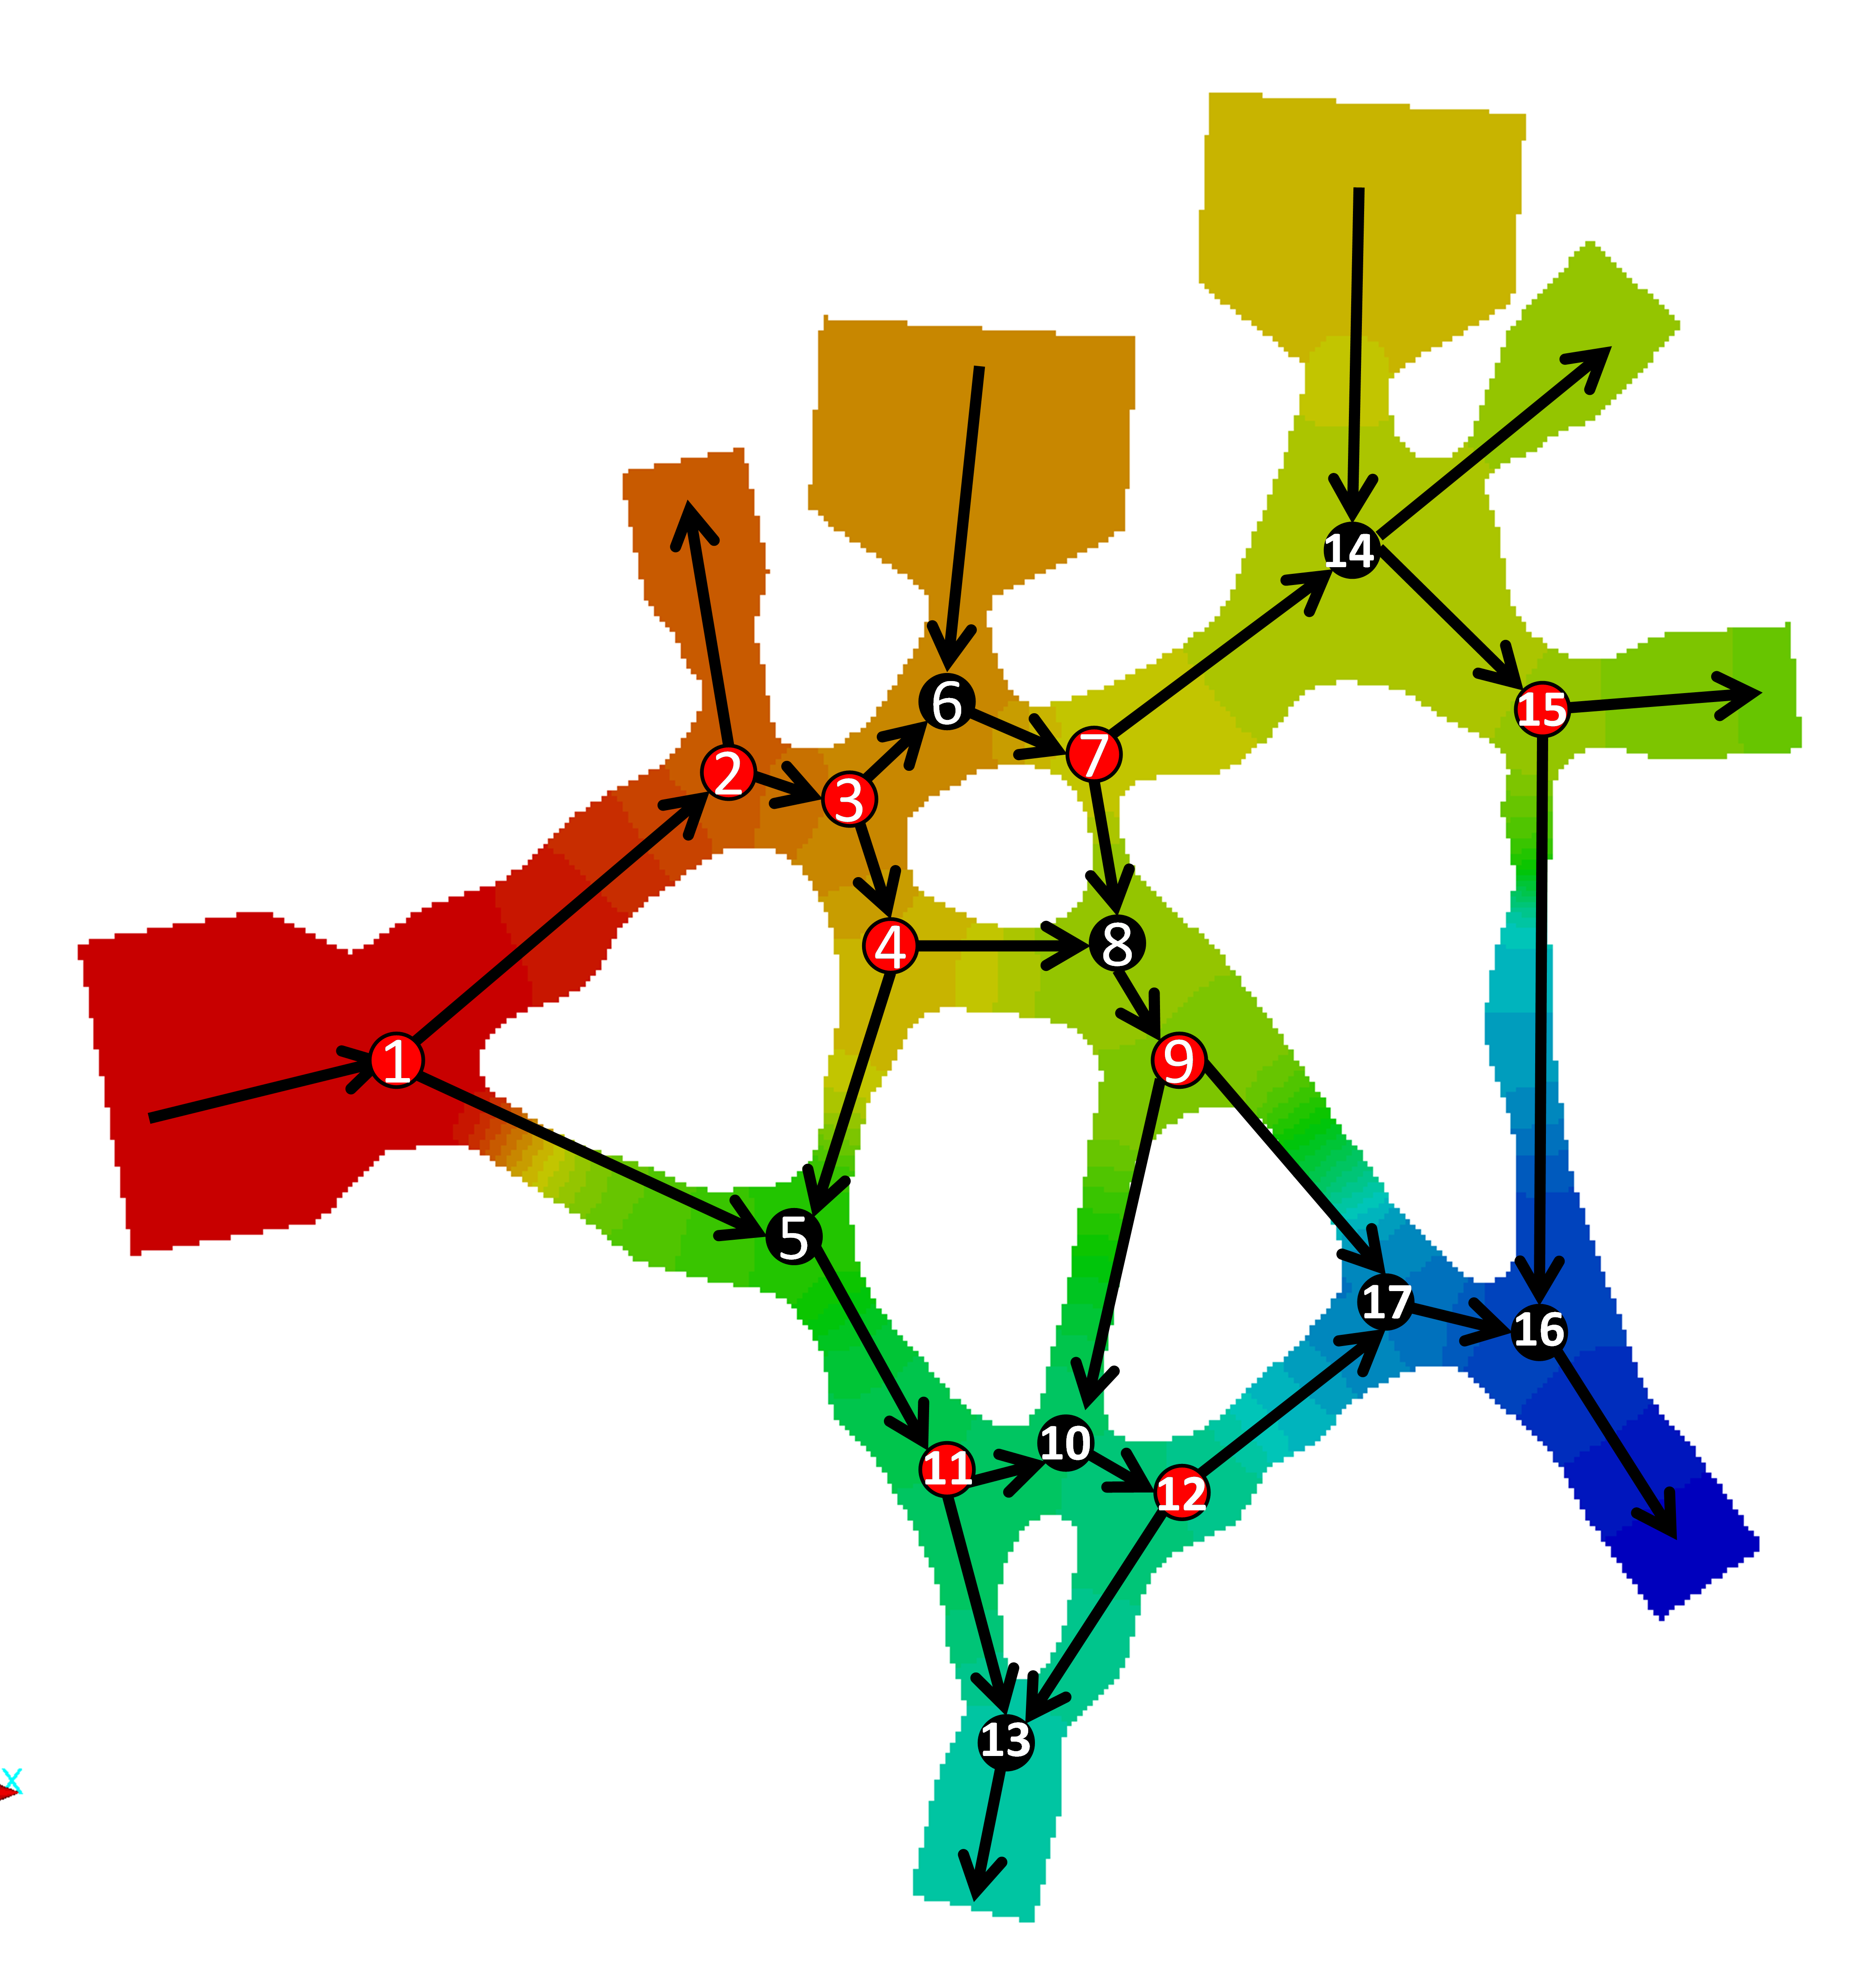
\includegraphics[width=1\textwidth]{images/bifurcations_ROI-2.png}
%     \caption{\textit{Schematic diagram of the ROI2 blood flow network which consists of 9 diverging bifurcations and 24 independent branches.} \label{ROI2}}
% \end{subfigure}
% \begin{subfigure}{0.33 \textwidth}
%     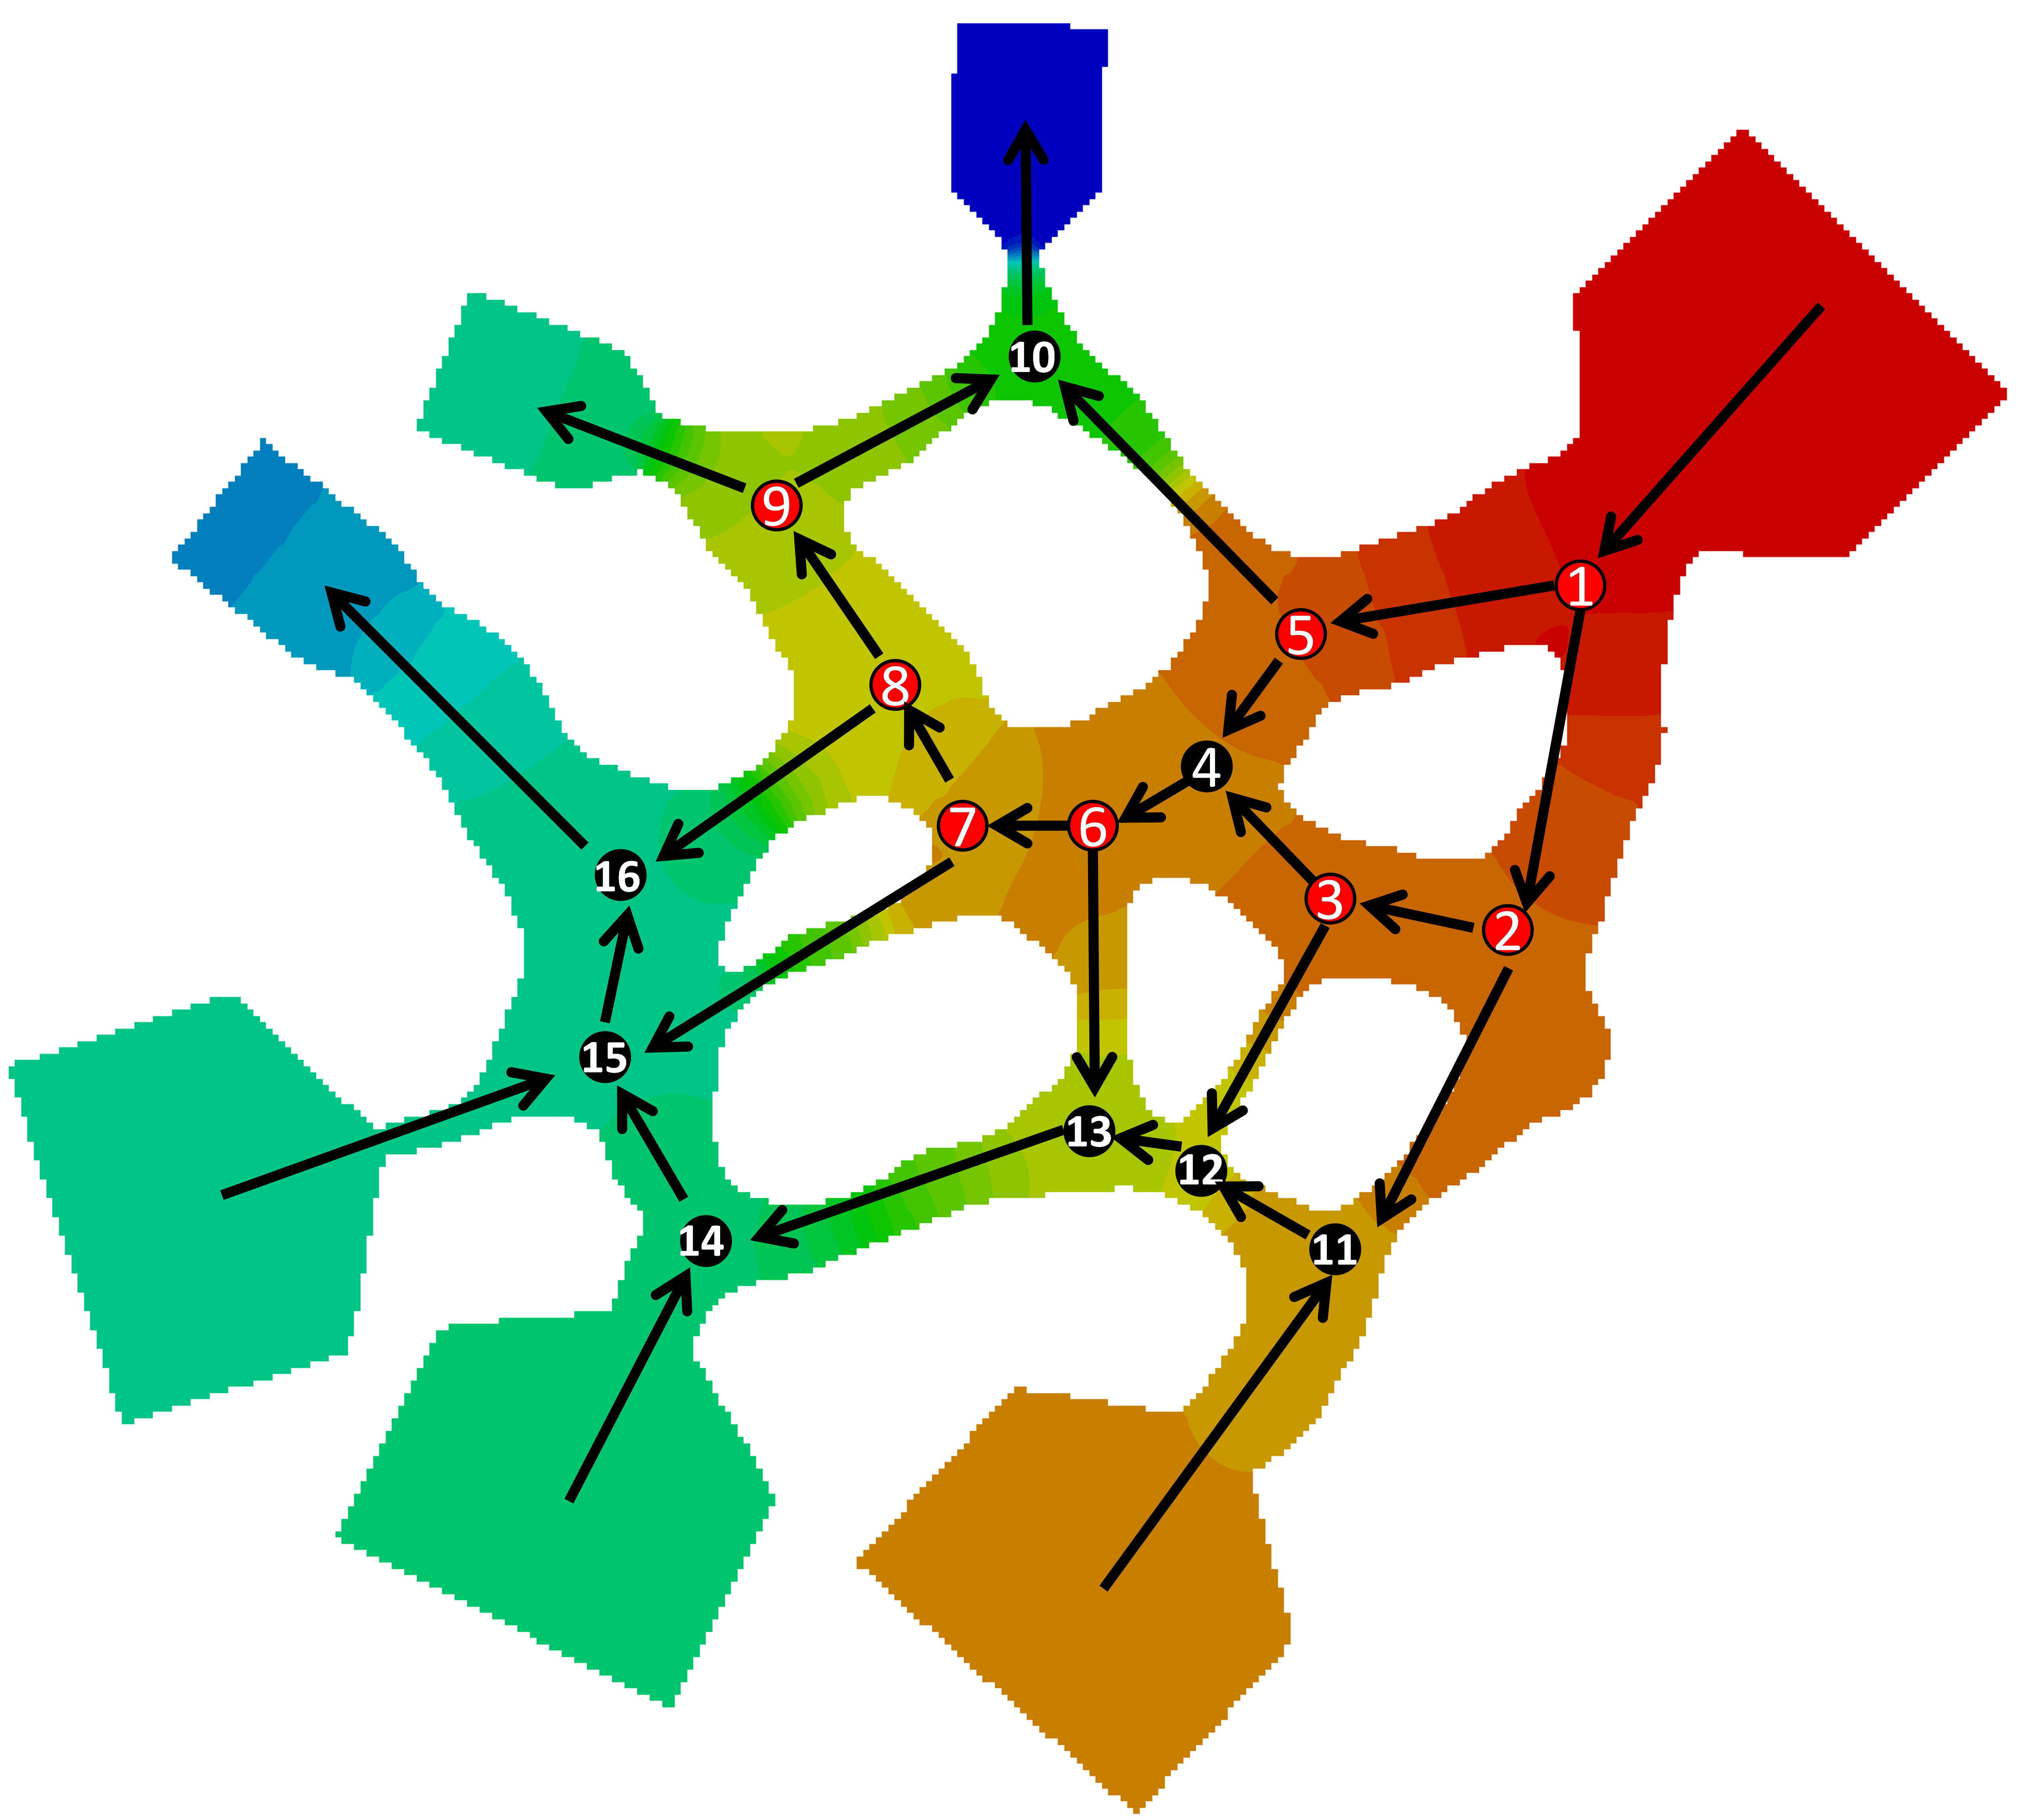
\includegraphics[width=1\textwidth]{images/bifurcations_ROI-3.png}
%     \caption{\textit{Schematic diagram of the ROI3 blood flow network which consists of 8 diverging bifurcations and 18 independent branches.} \label{ROI3}}
% \end{subfigure}
% \caption{\textit{Identification of flow patterns and diverging bifurcations within ROI-1, ROI-2 and ROI-3 respectively. The diverging bifurcations within each ROI are marked with red circles while the converging ones with black. The arrows indicate the direction of the blood flow in each individual branch, while the background contour points out the the pressure field where a warmer colour (E.g red) represents higher pressure.} \label{ROIs}}
% \end{figure}


\useportrait
\subsection{System Haematocrit in microvascular networks}
\label{SystemHaematocritInMicrovascularNetworks}
\begin{figure}[H]
\centering
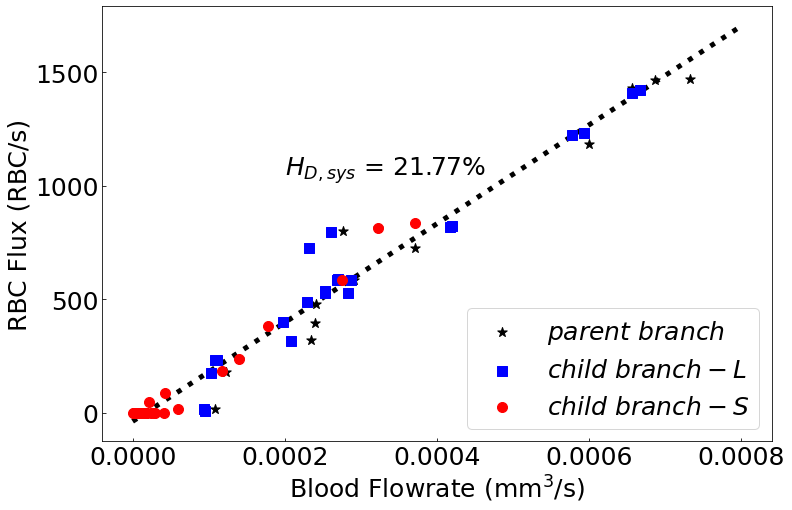
\includegraphics[width=0.95\textwidth]{images/SystemHaematocrit.png}
\caption{\textit{RBC flux against Blood flow rate including best-fit line. The "L"/"S" indicate the relatively larger (blue squares) and smaller (red circles) child branches in each diverging bifurcation respectively.} \label{SystemHaematocrit}}
\end{figure}


\subsection{Identification of Successive Bifurcations}
\begin{table}[H]
\centering
\caption{\textit{List of identified successive diverging bifurcations found across the micro-vascular networks. (see Figure \ref{ROIs}) BOIs with significant deviations between simulated fractional RBC flux to empirical predictions from PSM are indicated in red.}
\label{SuccessiveBOIs}}
\scalebox{1.2}{
\begin{tabular}{*{2}{c}}
\dtoprule
\textbf{ROIs} & \textbf{Successive BOI Combinations} \\
\midrule[0.5pt]
\multirow{3}{*}{ROI-1} & BOI-10 $\Rightarrow$ BOI-9 \\
& BOI-11 $\Rightarrow$ BOI-10 \\
& BOI-13 $\Rightarrow$ BOI-11 \\
\midrule[0.5pt]
\multirow{3}{*}{ROI-2} & BOI-1 $\Rightarrow$ BOI-2 \\
& BOI-2 $\Rightarrow$ \textcolor{red}{BOI-3} \\
& \textcolor{red}{BOI-3} $\Rightarrow$ \textcolor{red}{BOI-4} \\
\midrule[0.5pt]
\multirow{6}{*}{ROI-3} & \textcolor{red}{BOI-1} $\Rightarrow$ \textcolor{red}{BOI-2} \\
& \textcolor{red}{BOI-2} $\Rightarrow$ BOI-3 \\
& BOI-6 $\Rightarrow$ BOI-7 \\
& BOI-7 $\Rightarrow$ \textcolor{red}{BOI-8} \\
& \textcolor{red}{BOI-8} $\Rightarrow$ BOI-9 \\
& BOI-1 $\Rightarrow$ BOI-5 \\
\dbottomrule
\end{tabular}}
\end{table}


\uselandscape
\subsection{Evaluation of Simulation Data against Phase Separation Model}
\label{EvaluationOfSimulationDataVSPSM}
\begin{figure}[H]
\centering
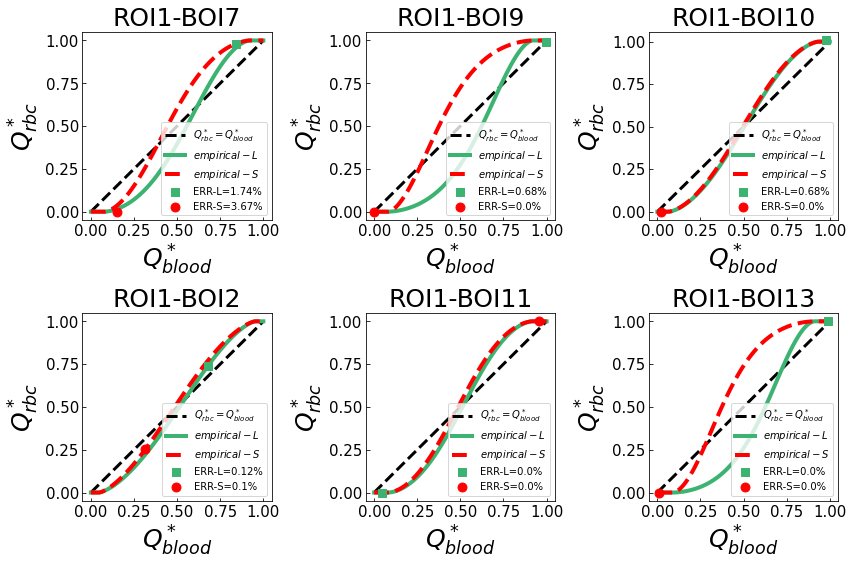
\includegraphics[width=0.775\textwidth]{images/DisproportionalityIndexQblood-ROI1.png}
\caption{\textit{Deviations between simulation data (squares/circle) and empirical predictions (solid lines) from PSM expressed as fractional RBC flux (Q$^{*}_{rbc}$) against fractional blood flow (Q$^{*}_{blood}$) for all selected diverging bifurcation within ROI-1. (see Figure \ref{ROIs}a) For each bifurcation, the "L" and "S" terms indicate the relatively larger (green coloured) and smaller (red coloured) child branches respectively. The black dotted line represents the linear theoretical line for Q$^{*}_{blood}$ and Q$^{*}_{rbc}$ without the presence of plasma skimming.} \label{DisproportionalityIndexQblood-ROI1}}
\end{figure}


\useportrait
\begin{figure}[H]
\centering
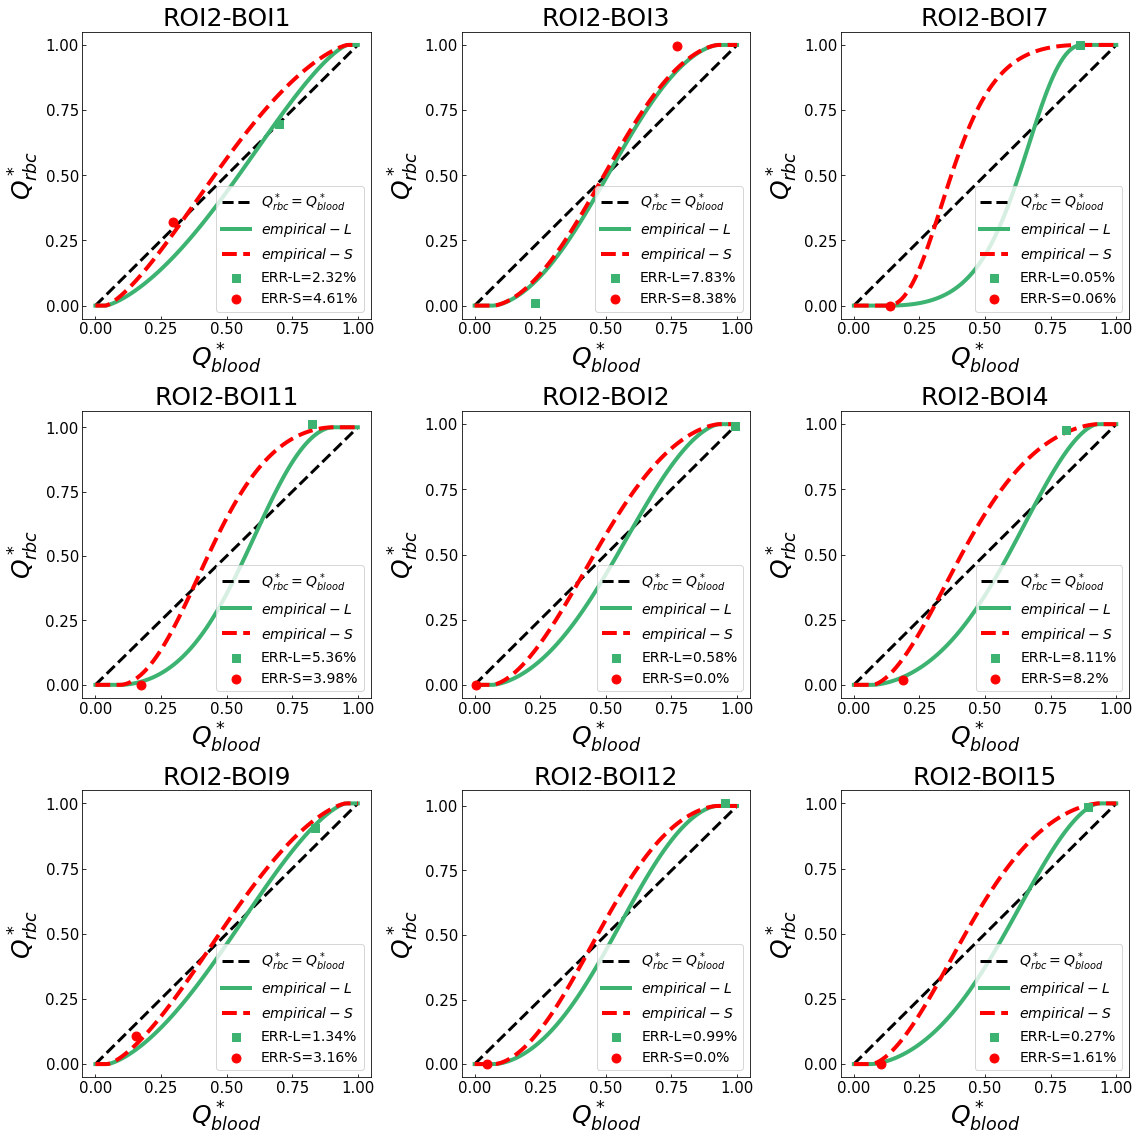
\includegraphics[width=1\textwidth]{images/DisproportionalityIndexQblood-ROI2.png}
\caption{\textit{Deviations between simulation data (squares/circle) and empirical predictions (solid lines) from PSM expressed as fractional RBC flux (Q$^{*}_{rbc}$) against fractional blood flow (Q$^{*}_{blood}$) for all selected diverging bifurcation within ROI-2. (see Figure \ref{ROIs}b) For each bifurcation, the "L" and "S" terms indicate the relatively larger (green coloured) and smaller (red coloured) child branches respectively. The black dotted line represents the linear theoretical line for Q$^{*}_{blood}$ and Q$^{*}_{rbc}$ without the presence of plasma skimming.} \label{DisproportionalityIndexQblood-ROI2}}
\end{figure}


\uselandscape
\begin{figure}[H]
\centering
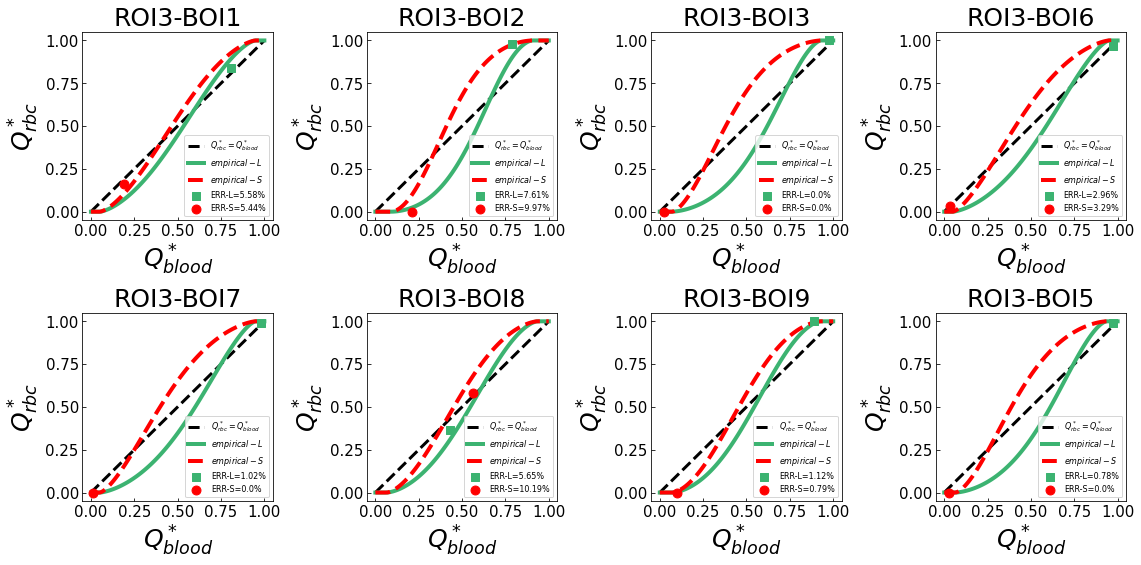
\includegraphics[width=1\textwidth]{images/DisproportionalityIndexQblood-ROI3.png}
\caption{\textit{Deviations between simulation data (squares/circle) and empirical predictions (solid lines) from PSM expressed as fractional RBC flux (Q$^{*}_{rbc}$) against fractional blood flow (Q$^{*}_{blood}$) for all selected diverging bifurcation within ROI-3. (see Figure \ref{ROIs}c) For each bifurcation, the "L" and "S" terms indicate the relatively larger (green coloured) and smaller (red coloured) child branches respectively. The black dotted line represents the linear theoretical line for Q$^{*}_{blood}$ and Q$^{*}_{rbc}$ without the presence of plasma skimming.} \label{DisproportionalityIndexQblood-ROI3}}
\end{figure}

\useportrait
\subsection{Evaluation of Simulation Data against Pries Viscosity Models}
\label{EvaluationOfSimulationDataVSPVM}
\begin{figure}[H]
\centering
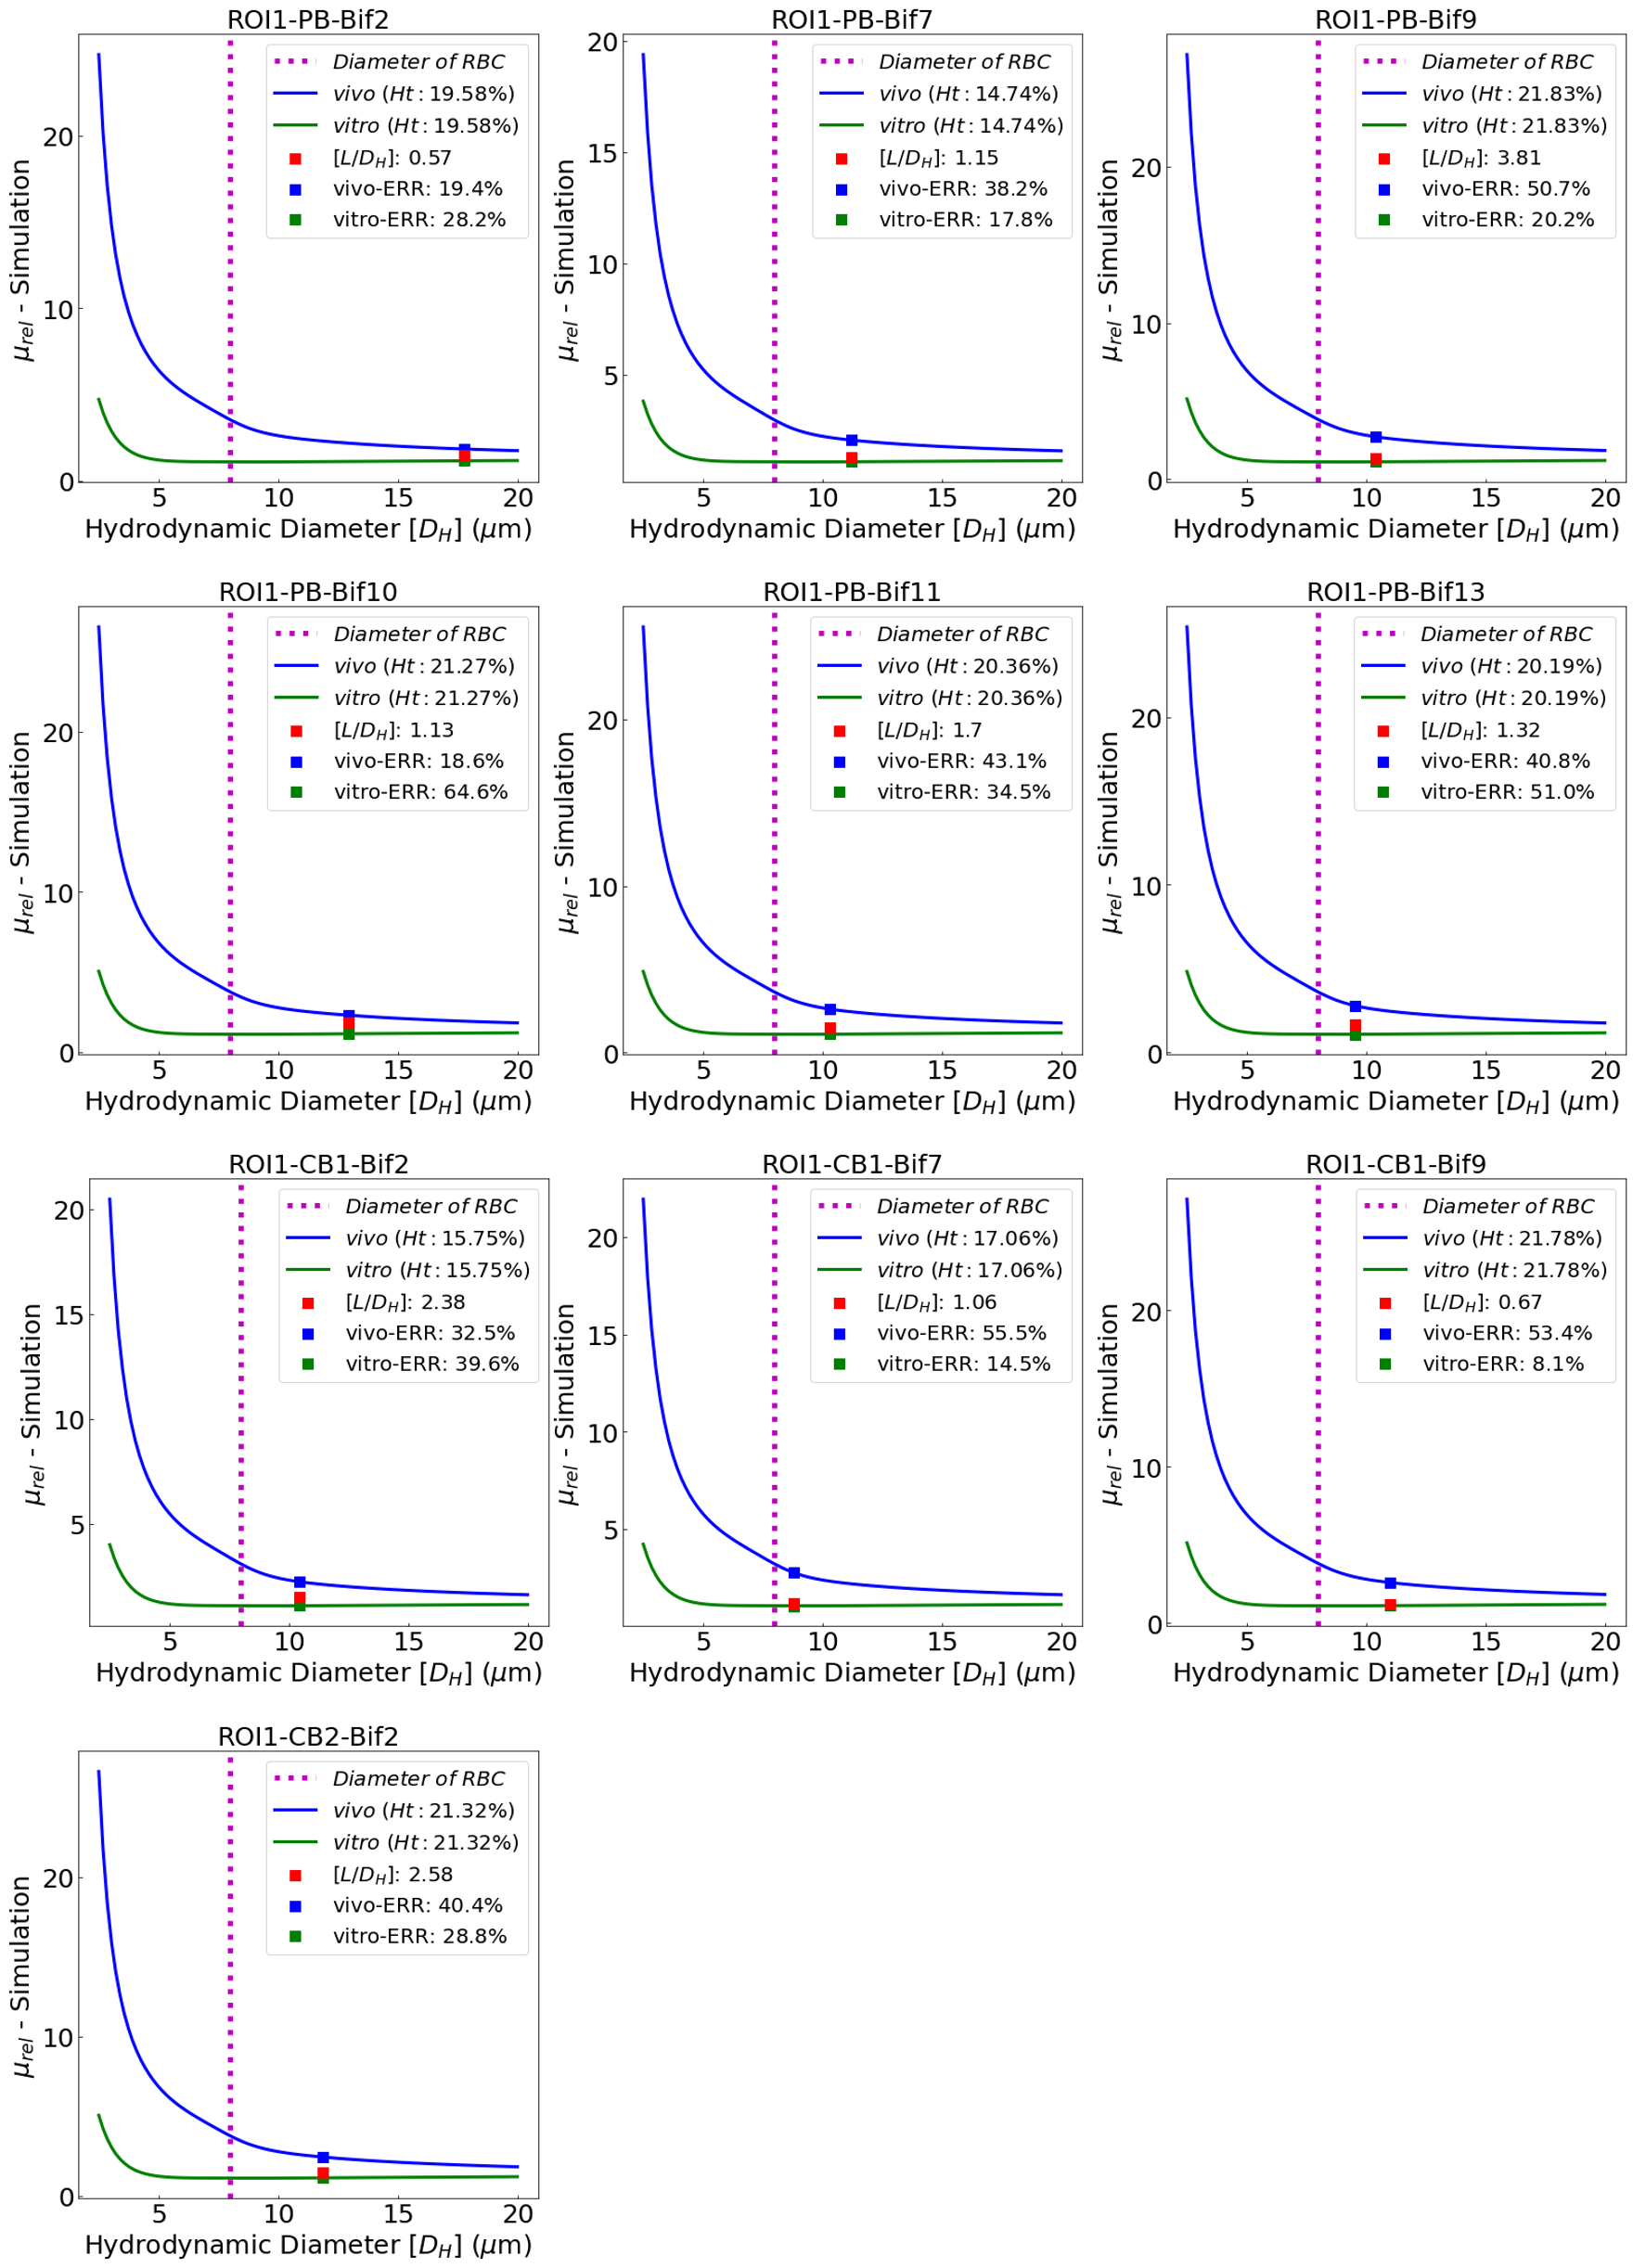
\includegraphics[width=0.925\textwidth]{images/DeviationsViscosity-ROI1.png}
\caption{\textit{Evaluation of non-zero haematocrit simulation data (red) against the empirical predictions (blue and green) from both in vivo and in vitro Pries Viscosity Models (solid lines) expressed as relative apparent viscosity ($\mu_{rel}$) against diameter (D$_{H}$) for each individual branch in ROI-1.(see Figure \ref{ROIs}a) The purple dotted line indicates the average diameter of a human RBC.} \label{DeviationsViscosity-ROI1}}
\end{figure}


\uselandscape
\begin{figure}[H]
\centering
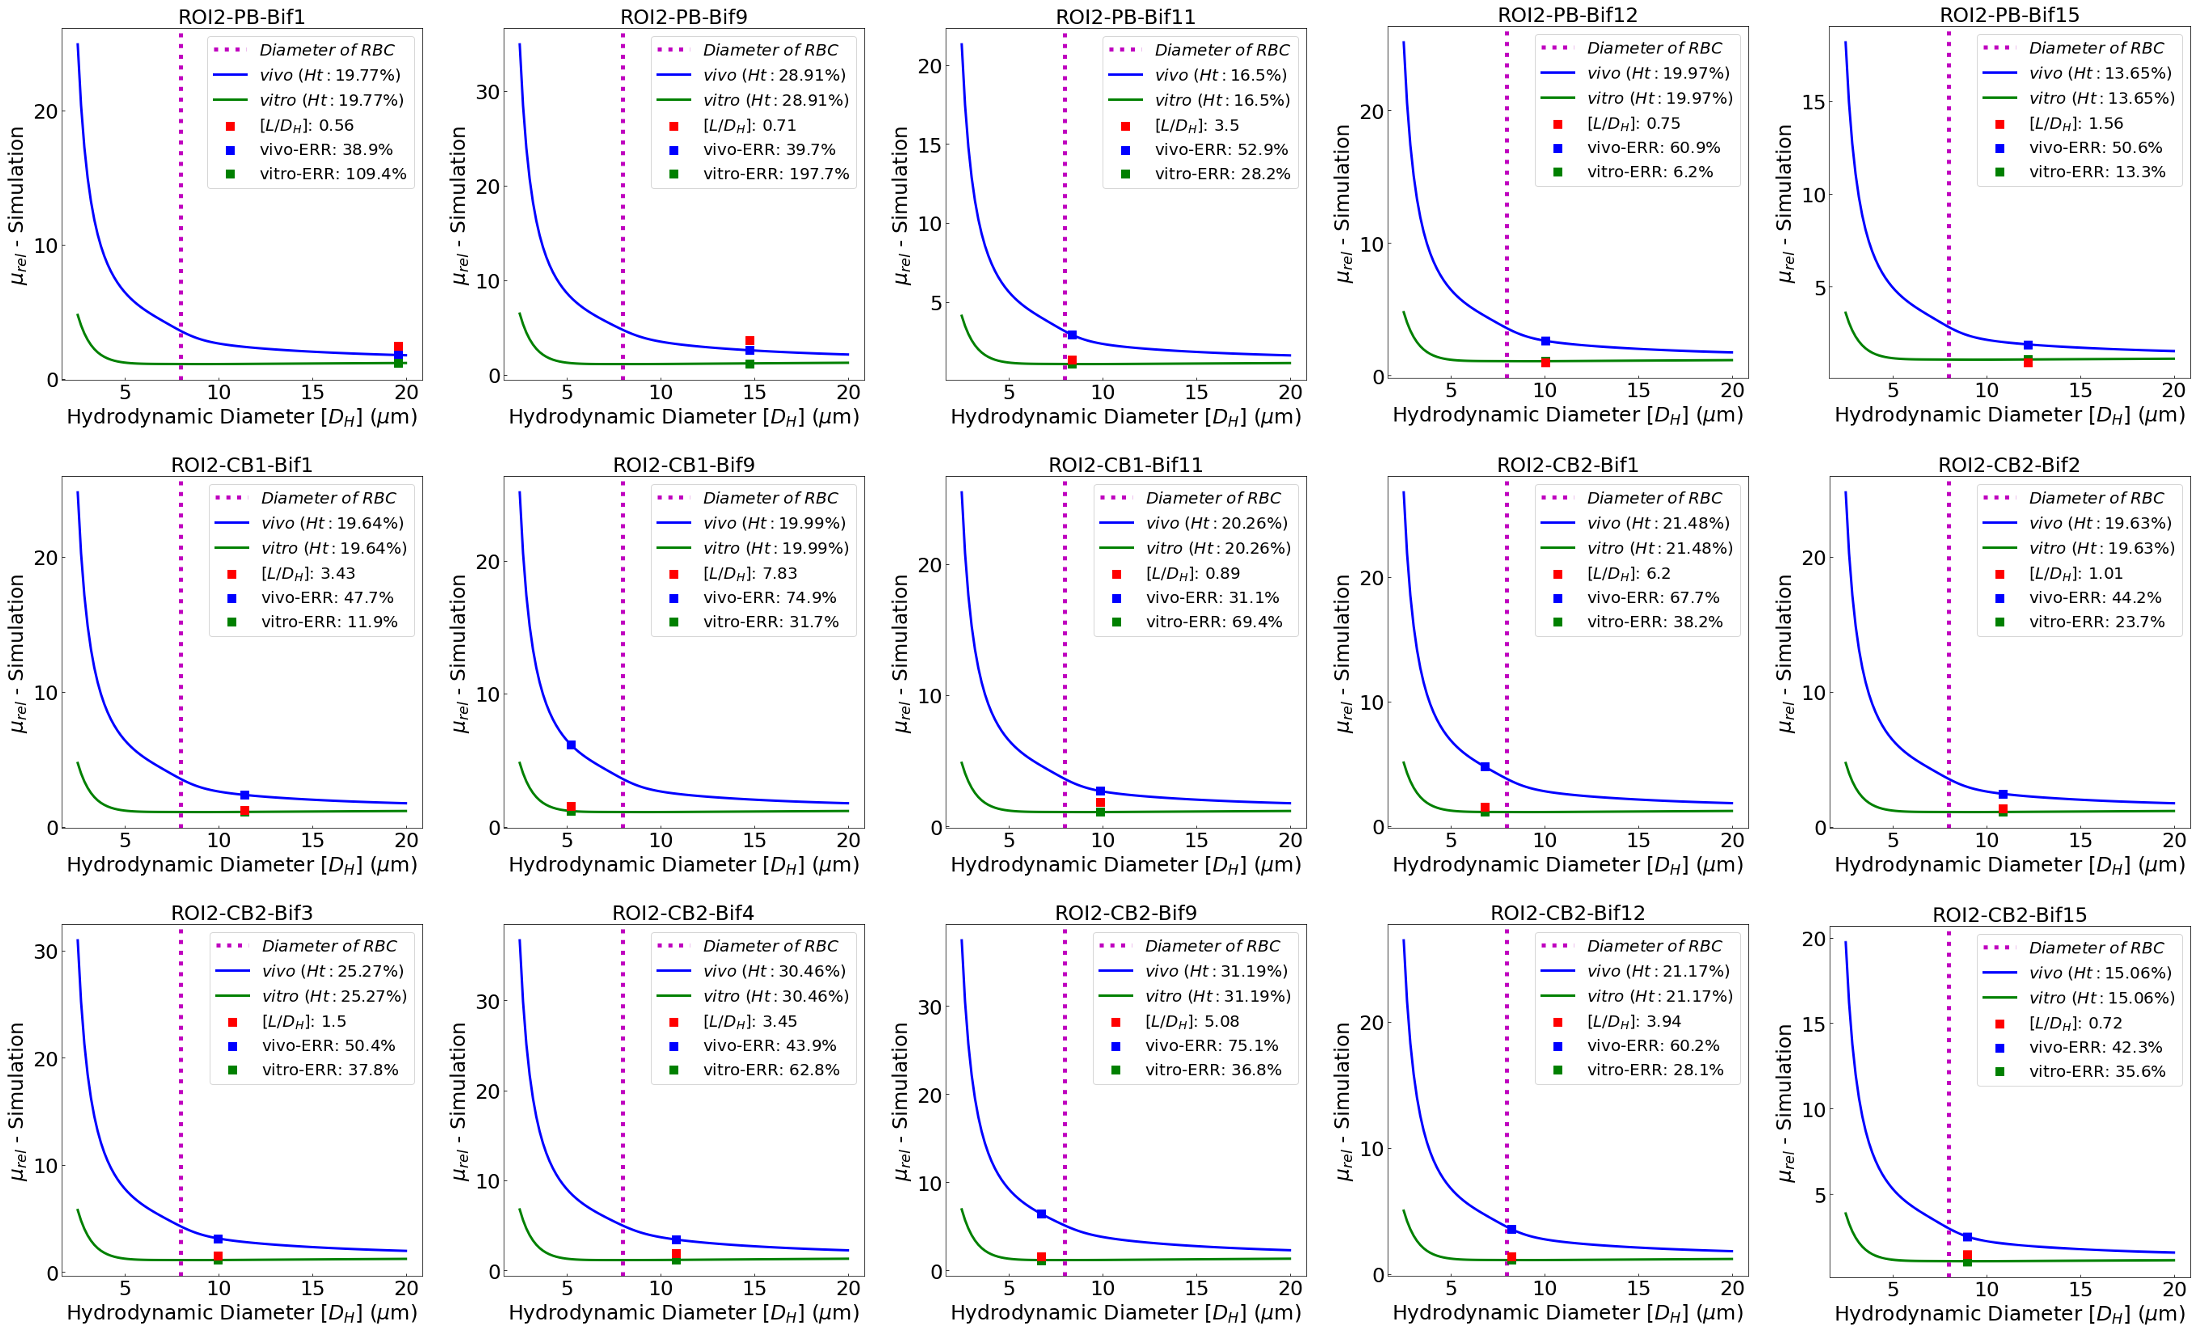
\includegraphics[width=0.95\textwidth]{images/DeviationsViscosity-ROI2.png}
\caption{\textit{Evaluation of non-zero haematocrit simulation data (red) against the empirical predictions (blue and green) from both in vivo and in vitro Pries Viscosity Models (solid lines) expressed as relative apparent viscosity ($\mu_{rel}$) against diameter (D$_{H}$) for each individual branch in ROI-2.(see Figure \ref{ROIs}b) The purple dotted line indicates the average diameter of a human RBC.} \label{DeviationsViscosity-ROI2}}
\end{figure}

\begin{figure}[H]
\centering
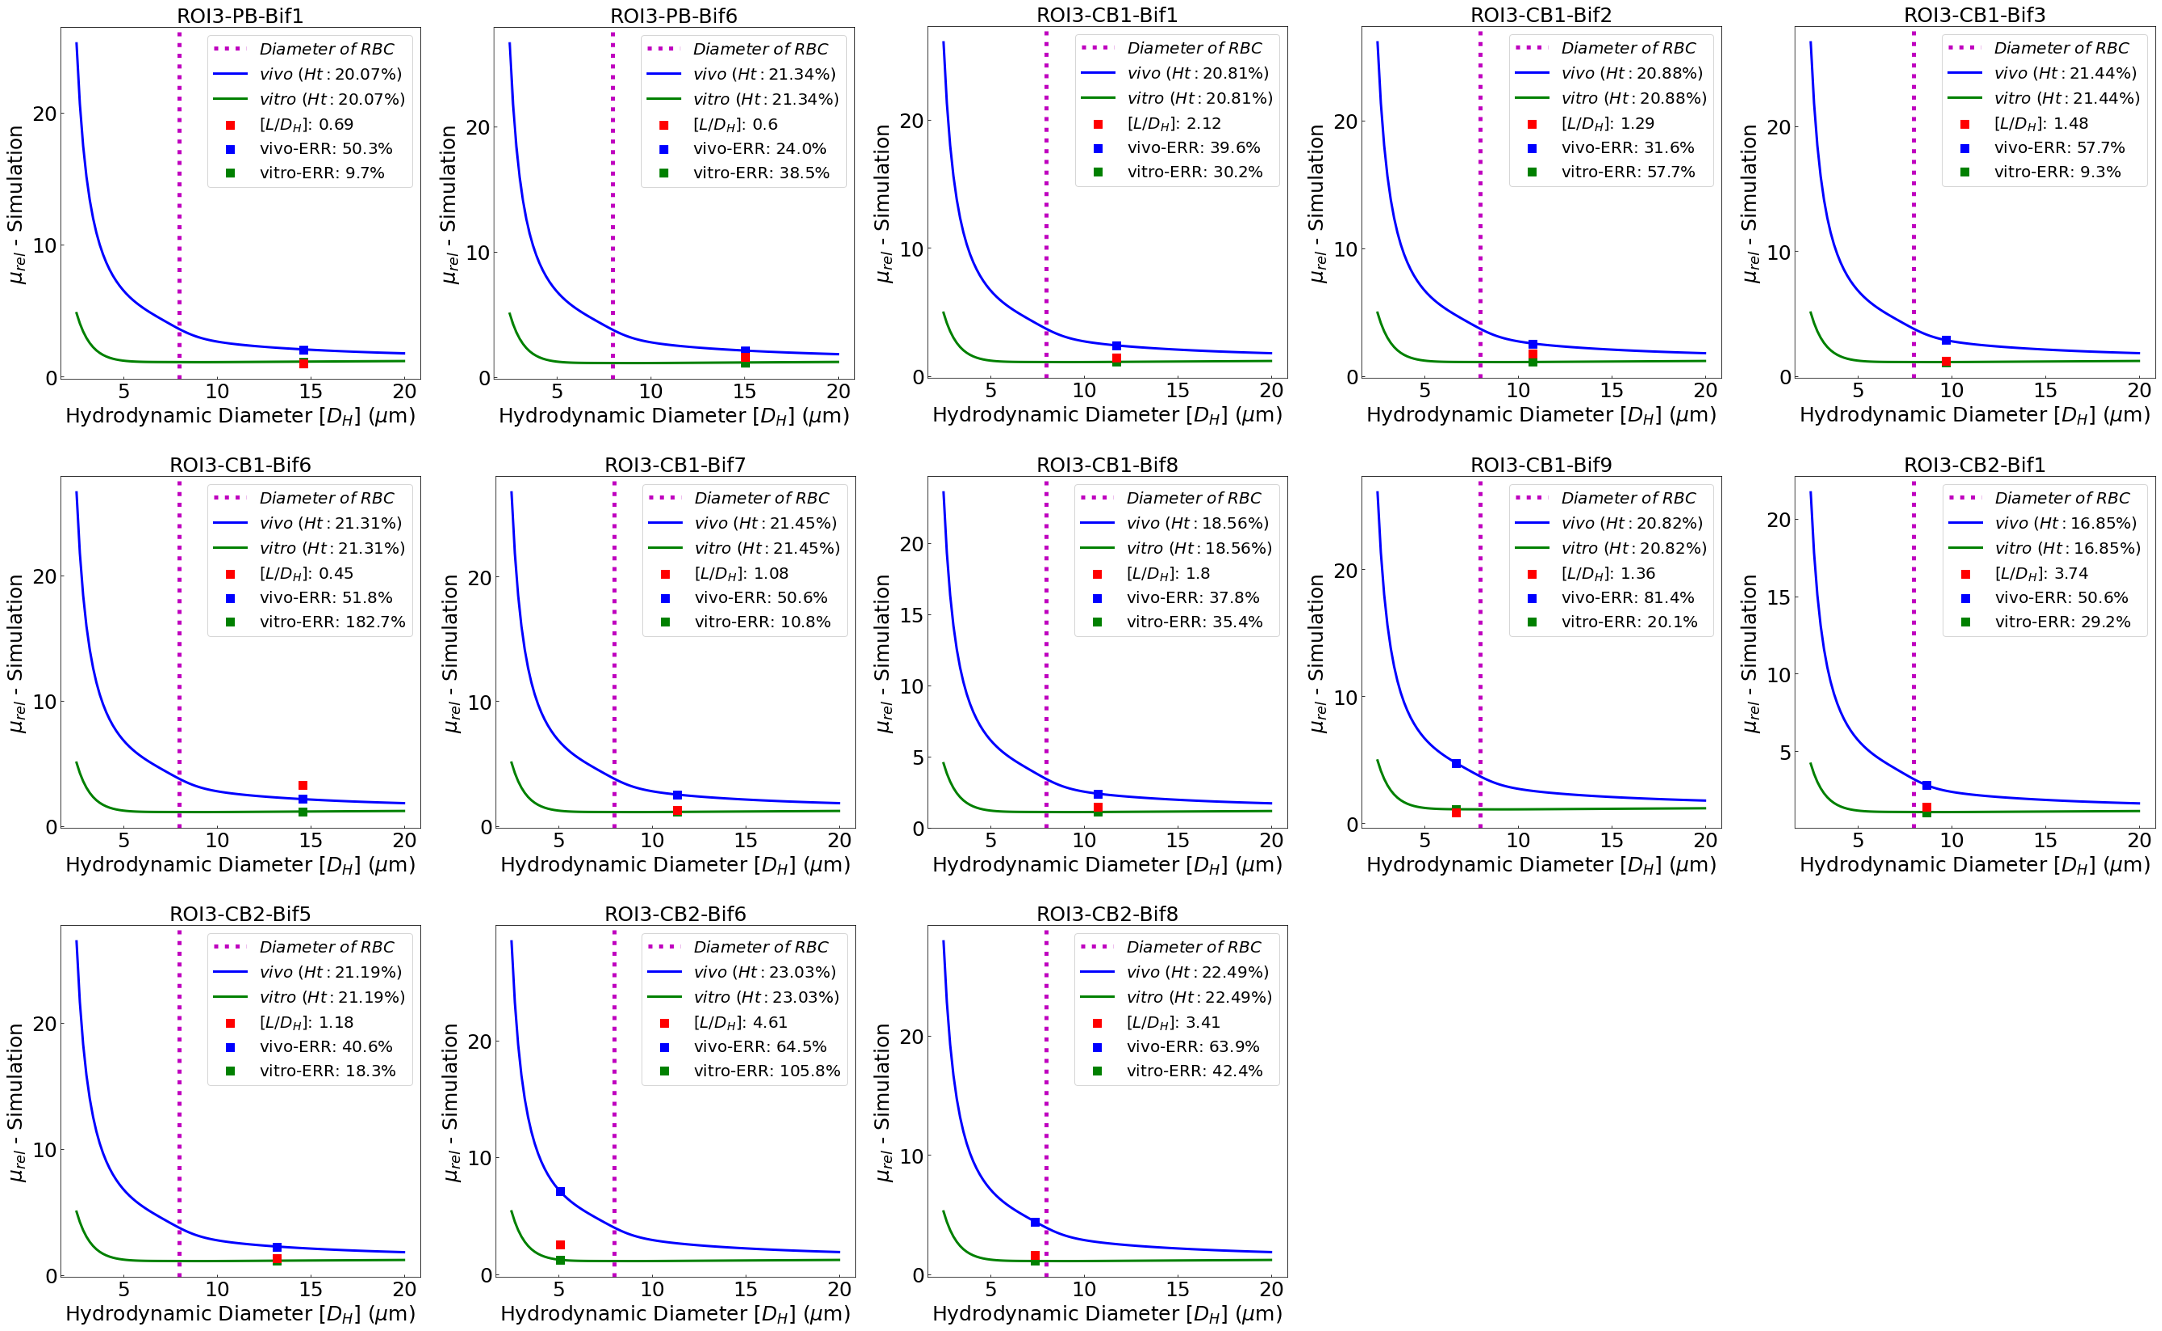
\includegraphics[width=0.95\textwidth]{images/DeviationsViscosity-ROI3.png}
\caption{\textit{Evaluation of non-zero haematocrit simulation data (red) against the empirical predictions (blue and green) from both in vivo and in vitro Pries Viscosity Models (solid lines) expressed as relative apparent viscosity ($\mu_{rel}$) against diameter (D$_{H}$) for each individual branch in ROI-3.(see Figure \ref{ROIs}c) The purple dotted line indicates the average diameter of a human RBC.} \label{DeviationsViscosity-ROI3}}
\end{figure}


\useportrait

\useportrait
\subsection{List of Outliers and Child Branches without any RBCs}
\begin{table}[H]
\centering
\caption{\textit{List of child branches without any RBCs found within the studied networks}
\label{CBwithoutRBCs}}
\scalebox{1.3}{
\begin{tabular}{*{3}{c}}
\dtoprule
\textbf{ROI1} & \textbf{ROI2} & \textbf{ROI3} \\
\midrule[0.5pt]
BOI7-CB2 & BOI2-CB1 & BOI2-CB2 \\
BOI9-CB2 & BOI7-CB2 & BOI3-CB2 \\
BOI10-CB1 & BOI11-CB2 & BOI5-CB1 \\
BOI11-CB2 & BOI12-CB1 & BOI7-CB2 \\
BOI13-CB1 & BOI15-CB1 & BOI9-CB2 \\
\dbottomrule
\end{tabular}}
\end{table}

\begin{table}[H]
\centering
\caption{\textit{List of outliers found within the studied networks}
\label{Outliers}}
\scalebox{1.3}{
\begin{tabular}{*{3}{c}}
\dtoprule
\textbf{ROI1} & \textbf{ROI2} & \textbf{ROI3} \\
\midrule[0.5pt]
BOI9-CB2 & BOI2-CB1 & BOI2-CB2 \\
BOI10-CB1 & BOI15-CB1 & BOI5-CB1 \\
BOI11-CB2 &  & BOI7-CB2 \\
\dbottomrule
\end{tabular}}
\end{table}

\useportrait
\end{appendices}


\end{document}
